\documentclass{article}
\usepackage{graphicx} % Required for inserting images


\author{Axel Flinth}
\date{January 2024}

\usepackage{amsmath}
\usepackage{amsfonts}
\usepackage{amsthm}
\usepackage{amssymb}

\newcommand{\g}{\mathfrak{g}}
\newcommand{\h}{\mathfrak{h}}

\usepackage[utf8]{inputenc} % allow utf-8 input
\usepackage[T1]{fontenc}    % use 8-bit T1 fonts
\usepackage{hyperref}       % hyperlinks
\usepackage{url}            % simple URL typesetting
\usepackage{booktabs}       % professional-quality tables
\usepackage{amsfonts}       % blackboard math symbols
\usepackage{nicefrac}       % compact symbols for 1/2, etc.
\usepackage{microtype}      % microtypography
\usepackage{xcolor}         % colors


\usepackage{geometry}[top=2cm,bottom=2cm,left=2cm,right=2cm]

%%%%%%%%%%%%%%%%%%%%%%%%%%%%%%%%%% OUR PACKAGES %%%%%%%%%%%%%%%%%%%%%%%%%%%%%%%%%%%%%%%%%%%
\usepackage{amsmath}
\usepackage{amsthm}
\usepackage{enumerate}
\usepackage{graphicx}
\usepackage{caption}
\usepackage{subcaption}
\usepackage{dsfont}
\usepackage{xfrac}
\usepackage{algorithm}
\usepackage{algorithmic} 

\DeclareMathOperator*{\argmin}{arg\,min}

%%%%%%%%%%%%%%%%%%%%%%%%%%%%%%%%%%% OUR MACROS %%%%%%%%%%%%%%%%%%%%%%%%%%%%%%%%%%%%%%%%%%%%
\newcommand{\aug}{\mathrm{aug}}
\newcommand{\FA}{\mathrm{FA}}
\newcommand{\End}{\mathrm{End}}
\newcommand{\Hom}{\mathrm{Hom}}
\newcommand{\erw}{\mathbb{E}} % Av gammal vana använder jag(Axel) macrot \erw ('Erwartungswert') för väntevärde
\newcommand{\id}{\mathrm{id}}
\newcommand{\ad}{\mathrm{ad}}
\newcommand{\Ad}{\mathrm{Ad}}
\newcommand{\dd}{\mathrm{d}}
\newcommand{\res}{\mathrm{res}}
\newcommand{\eqv}{\mathrm{eqv}}
\newcommand{\tr}{\mathrm{tr}}
\newcommand{\tensortwo}{{\otimes 2}}
\newcommand{\otensor}{\otimes}
\newcommand{\hess}{\nabla^2}
\newcommand{\spec}{\mathrm{spec}}
\newcommand{\indrho}{\overline{\rho}}
\newcommand{\diag}{\mathrm{diag}}
\DeclareMathOperator{\supp}{\mathrm{supp}}

\newcommand{\perm}{\mathrm{perm}}
\newcommand{\trans}{\mathrm{tr}}
\newcommand{\rot}{\mathrm{rot}}

\newcommand{\calA}{\mathcal{A}}
\newcommand{\calC}{\mathcal{C}}
\newcommand{\calD}{\mathcal{D}}
\newcommand{\calF}{\mathcal{F}}
\newcommand{\calH}{\mathcal{H}}
\newcommand{\calL}{\mathcal{L}}
\newcommand{\calI}{\mathcal{I}}
\newcommand{\calE}{\mathcal{E}}
\newcommand{\sprod}[1]{\langle #1 \rangle}
\newcommand{\calW}{\mathcal{W}}
\newcommand{\calS}{\mathcal{S}}
\newcommand{\calU}{\mathcal{U}}
\newcommand{\calN}{\mathcal{N}}

\newcommand{\K}{\mathbb{K}}
\newcommand{\R}{\mathbb{R}}
\newcommand{\N}{\mathbb{N}}
\newcommand{\Z}{\mathbb{Z}}
\newcommand{\C}{\mathbb{C}}
\renewcommand{\S}{\mathbb{S}}
\renewcommand{\P}{\mathbb{P}}

\newcommand{\su}{\mathfrak{su}}
\renewcommand{\sp}{\mathfrak{sp}}
\newcommand{\so}{\mathfrak{so}}
\newcommand{\gl}{\mathfrak{gl}}
\renewcommand{\sl}{\mathfrak{sl}}

\newcommand{\GL}{\mathrm{GL}}
\newcommand{\SU}{\mathrm{SU}}
\newcommand{\SL}{\mathrm{SL}}
\newcommand{\SO}{\mathrm{SO}}
\newcommand{\SP}{\mathrm{SP}}


\newcommand{\sse}{\subseteq}

\newtheorem{example}{Example}
\newtheorem{assumption}{Assumption}
\newtheorem{remark}{Remark}
\newtheorem{lemma}{Lemma}
\newtheorem{theorem}{Theorem}
\newtheorem{cor}{Corollary}
\newtheorem{prop}{Proposition}
\newtheorem{defi}{Definition}
\newtheorem{exercise}{Exercise}

\newcommand{\set}[2]{\{ #1 \, \vert \, #2\}}
\newcommand{\abs}[1]{\vert #1 \vert}
\newcommand{\norm}[1]{\Vert #1 \Vert}

\renewcommand{\div}{\mathrm{div}}

\newcommand{\python}[1]{\texttt{#1}}
\newcommand{\ReLU}{\mathrm{ReLU}}
\newcommand{\softmax}{\mathrm{softmax}}
\newcommand{\sigmoid}{\mathrm{sigmoid}}
\newcommand{\one}{\mathds{1}}
\newcommand{\leqsim}{\lesssim}
\DeclareMathOperator{\sgn}{sgn}
\DeclareMathOperator{\dist}{dist}

\newcommand{\weak}{\mathrm{weak}}

\usepackage{tikz}
\usetikzlibrary{matrix,arrows.meta}
\usepackage{wrapfig}


\begin{document}
\begin{center}

    {\Large Statistical learning with high-dimensional data (5MS084)\\

    \vspace{1.5cm}
    
    Winter term 2025 \\

 \vspace{1.5cm}
    
    
\includegraphics[width=.3\textwidth]{graphics/umu.png}

  \vspace{1.5cm}
    
    Axel Flinth}
   
\end{center}

\tableofcontents

These lecture notes are heavily inspired by the excellent book \cite{james2023introduction}.

\newpage


\section{Elements of machine learning}
\emph{Machine learning} has had an immense impact on the world during the last decades. It is part of what some call a \emph{fourth industrial revolution} \cite{SchwabIndustry}, and is already influencing many people's daily life. The buzzword \emph{Artificial Intelligence} is mesmerizing, promising a world where machines with superhuman capabilities revolutionizes the way we live our lives.

\emph{Machine learning} at a first glance seems very esoteric. Words used for very human and lifelike processes are suddenly used for procedures related to such lifeless things as computers. Computers can suddenly \emph{learn} tasks? We \emph{train} them using data we have collected. We create \emph{intelligence} artificially. We should surely not go in to the philosophical aspects of AI -- this is not the scope of this course -- but we shall definitely begin by demystifiying a bit. \emph{Learning} and \emph{training} are merely descriptions of very technical and mathematical procedures, that while they can do marvelous things, are not at all magical.


\subsection{The setting of statistical learning}
The principle of \emph{machine learning} is most easily described through so-called \emph{supervised learning tasks}. In this setting, we imagine \emph{data points} $x_i$ in some set $X$
being attached with \emph{labels} $y_i$ in some other set $Y$. Examples include 
\begin{itemize}
    \item images labeled with descriptions (from some fixed set)
    \item positions, sizes, ages of houses, labeled with their market prices
    \item gene expression data from patients, labelled with data if they are sick or not 
\end{itemize}
The first and third task here are classification problems, whereas the second is a regression problem.
The task of statistical learning is to design a statistical model that given an unseen example $x_i \in X$ can accurately predict its label $y_i$. (This is fundamentally different from so-called \emph{unsupervised} tasks, where we are only given data $x_i$ in $X$, and our task is to group them into a number of classes. We will treat them later in the course).

We imagine that there is a (possibly very complicated)  mapping $f_*:X \to Y$ (a \textbf{ground truth}) that returns the label to any example. When observing labels of training examples, there will always be errors, so that we should model the relation between the training examples and errors as follows
\begin{align}
    y_i = f_*(x_i) + \varepsilon_i, \label{eq:model}
\end{align}
where $\varepsilon_i$ is some random error. \textbf{The fundamental task of statistical learning is to infer $f_*$ from finitely pairs $(x_i,y_i)$ available to us}. The $(x_i,y_i)$ pairs are called the \textbf{training data}.

A natural strategy is to try to find the function $f$ that 'fits' the training data the best -- the hope is that this function will generalize well also to unseen data. A general technique for doing this is to pick a function $\ell: Y \times Y \to \R$ that measures the error between two labels (a \textbf{loss}) and then pick the function that minimizes the \textbf{empirical risk} (or \textbf{training error})
\begin{align*}
    R_e(f) = \tfrac{1}{n} \sum_{i \in [n]} \ell(f(x_i),y_i).
\end{align*}
If the labels are point in a Euclidean space $\R^m$, the loss can be the standard $\ell_2$-norm, for instance. One speaks of \textbf{empirical risk minimization}, ERM. Note that the empirical risk is an approximation of the 'true risk'. 
\begin{align*}
    R(f) = \mathbb{E}(\ell(f(x),y)),
\end{align*}
where the expectation is taken with respect to the distribution of $(x,y) \in X \times Y$ -- our training data are samples from this distribution. Note that this can be seen as 'testing' the model on unseen data -- therefore, we will often refer to it as the test risk or \textbf{test error}.

Minimizing over all functions $f$ is most often not feasible -- there are simply too many functions to test -- and also not very wise, for reasons we will come back to later. Therefore, one specifies a \textbf{hypothesis class} of feasible functions, say $\calF$, and chooses the best function from the class via \textbf{empirical risk} minimization (ERM) 
\begin{align*}
    \hat{f} = \argmin_{f\in \calF} R_e(f).
\end{align*}
Solving (approximately) this problem (or rather a problem of this type) is the meaning of \textbf{training} a \textbf{model}.

\begin{figure}
    \centering
    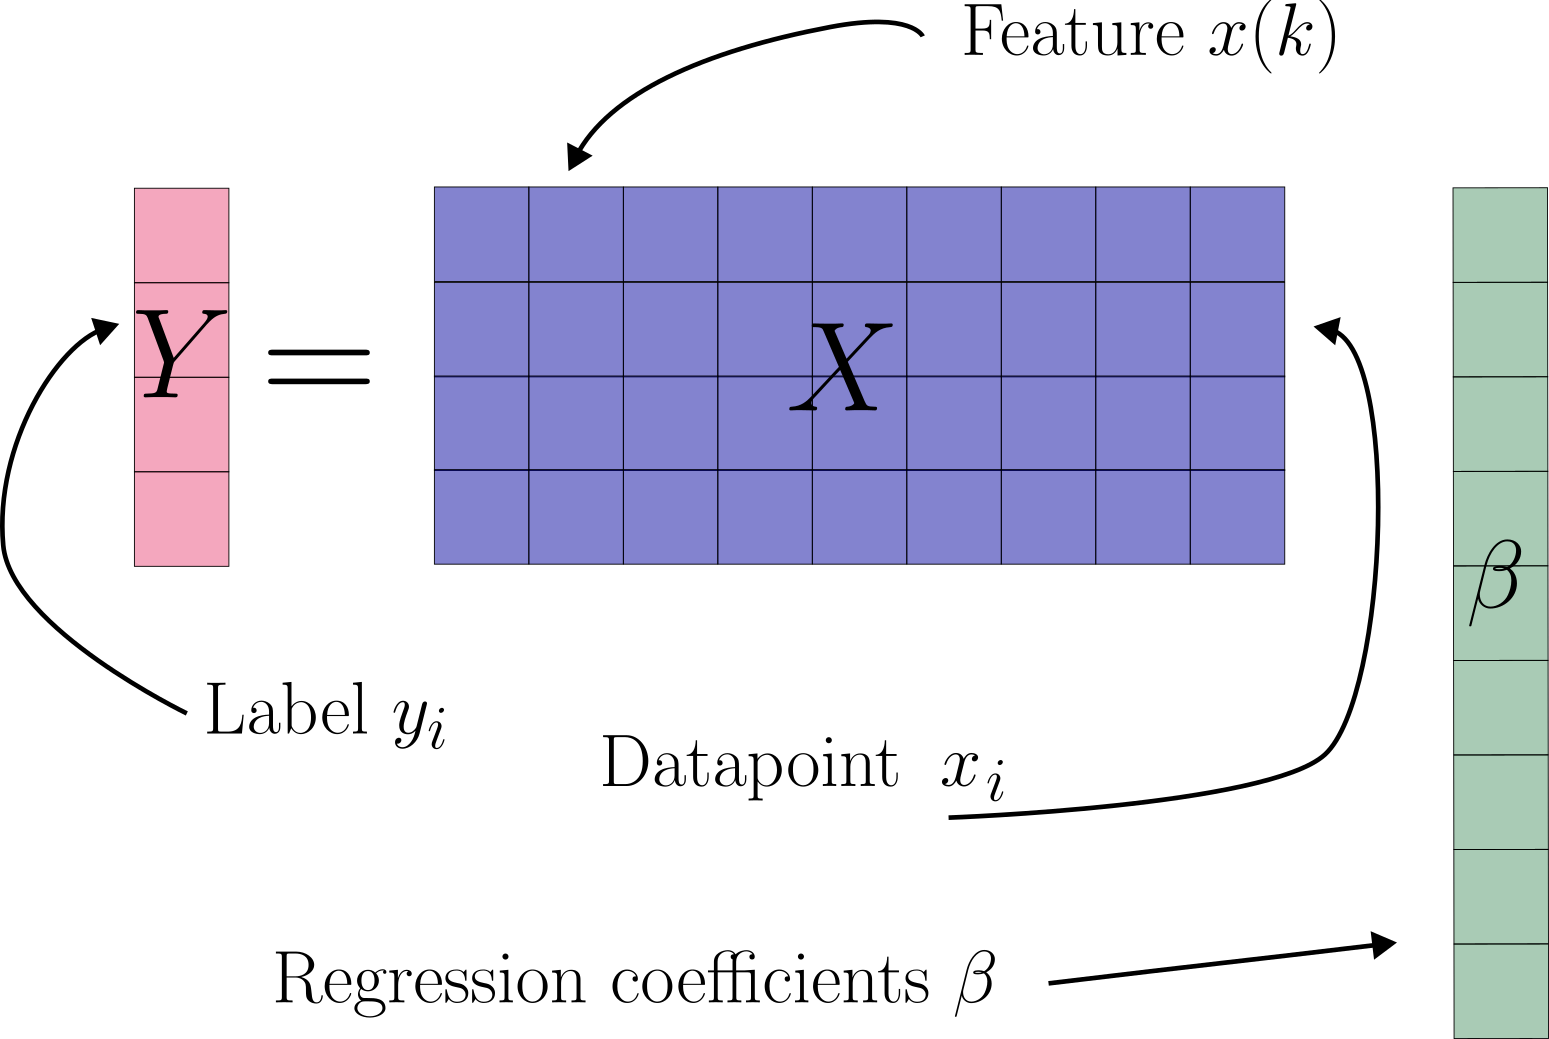
\includegraphics[width=0.5\linewidth]{graphics/linear_regression.png}
    \caption{The matrix-vector notation of the linear regression problem}
    \label{fig:linreg}
\end{figure}

\paragraph{Example: Linear regression} In this class, we will encounter many different hypothesis classes, or models. As an illustrative example, we can think about \emph{linear regression}. Here, the data are tuples of real numbers(features) -- i.e. $x_i \in \R^p$ for some $p$ -- the labels are real numbers $y_i \in \R$ and hypothesis class is the set of all (affine-)linear functions from $\R^p \to \R$, i.e.
\begin{align*}
    \calF_{\mathrm{lin}} = \{x \mapsto a + \sprod{\beta, x} \, \vert \, a \in \R, \beta \in \R^p\}
\end{align*}
If we're using a quadratic loss (which is standard), the empirical risk minimization takes the form
\begin{align*}
    \min_{a\in \R, \beta \in \R^p} \tfrac{1}{n} \sum_{i \in [n]} (a + \sprod{\beta,x_i} - y_i)^2.
\end{align*}
Note that this can be written in matrix form: if we let $Y$ be the vector with $i$:th entry $y_i$, $\overline{X}$ the matrix with $i$:th row $(1,x_i)$ and $\one$ the vector with only ones, the above is equivalent to 
\begin{align*}
    \min_{\gamma \in \R^{p+1}} \norm{\overline{X}\gamma -Y}_2^2.
\end{align*}
This problem is, as we all know, relatively easy to solve with a computer: solutions are characterized by the linear equations
\begin{align*}
    \overline{X}^*\overline{X}\gamma = \overline{X}^*Y.
\end{align*}

\subsection{Bias-variance tradeoff}
Which hypothesis class $\calF$ to choose depends on a lot of things -- among them are practical issues, such as the complexity of solving the ERM -- but a general guiding principle is given to us by the so-called \textbf{bias-variance} trade-off. To explain it, let us introduce some more notation. First, let us call the (random) data $(x_i,y_i)$ $D$, and the function obtained by training the model on the data $D$ $f_D$ (it can be obtained through empirical risk minimization, but also by some other method). This function will depend on the data, but it will give us an estimate on average:
\begin{align*}
    \widehat{f}(x) = \mathbb{E}_D f_D(x).
\end{align*}
The expectation here is with respect to the \emph{random draw of the data}.

This mean estimate should optimally be close to the ground truth $f_*$, but this is not guaranteed (for instance, $f_*\notin \calF$ in general). In general, there is hence a discrepancy between the mean estimate $\widehat{f}$ and the ground truth $f_*$. This error is referred to as the \textbf{bias} of the model
\begin{align*}
    \mathrm{Bias}(f) = \mathbb{E}_x(\ell(\widehat{f}(x),f_*(x))).
\end{align*}

Now, the actual estimator $f_D$ we learn is not equal to the average $\widehat{f}$, but varies. We measure how much with the help of the \textbf{variance}:
\begin{align*}
    \mathrm{Var}(f) = \mathbb{E}_x \mathbb{V}_D(f_D(x))) = \mathbb{E}_x \mathbb{E}_D(f_D(x)-\widehat{f}(x))^2
\end{align*}
where both here and above, the 'error measuring data' $x$ is independent of the draw of the training data $D$. 

There is a fundamental relation between bias, variance and expected risk of a model:
\begin{theorem}
    Assume that the error $\epsilon$ is independent of the (train and test) data $x$, and centered: $\erw(\epsilon)=0$. Then, for the square loss, $\ell(y,y')=(y-y')^2$, the expected risk decomposes as follows:
    \begin{align*}
        \erw_D R(f_D) = \mathrm{Bias}(f) + \mathrm{Var}(f) + \mathrm{Var}(\epsilon).
    \end{align*}
\end{theorem}
\begin{proof}
    For each fixed $x$, we have
    \begin{align*}
        \ell(f_D(x),y) =& (f_D(x)-f_*(x)-\epsilon)^2 = \left((f_D(x) - \widehat{f}(x)) + (\widehat{f}(x)-f_*(x)) -\epsilon\right)^2 \\
        =& (f_D(x)-\widehat{f}(x))^2 + (\widehat{f}(x)- f_*(x))^2 +\epsilon^2 \\
        & +2 \epsilon (f_D(x)-\widehat{f}(x)) + 2\epsilon (\widehat{f}(x)- f_*(x)) + 2(\widehat{f}(x)- f_*(x))(f_D(x)-\widehat{f}(x))
    \end{align*}
    The three leading terms in the final expression are, after taking the expectation over $x$ and $D$, equal to $\mathrm{Var}(f)$, $\mathrm{Bias}(f)$ and $\mathrm{Var}(\epsilon)$, respectively. We hence only need to argue that the final three terms vanish. But this is easy -- since $\epsilon$ is independent of the data, we have
    \begin{align*}
        \erw_D(\epsilon ((\widehat{f}(x)- f_*(x))) = 2\erw_D(\epsilon) \erw_D((\widehat{f}(x)- f_*(x))) = 0 \cdot  \erw_D((\widehat{f}(x)- f_*(x))) =0,
    \end{align*}
    and likewise for the other term, since $\epsilon$ is centered. As for the final term, notice that $(\widehat{f}(x)- f_*(x))$ actually does not depend on the data -- $\widehat{f}$ is the expected value of $f_D$ over the draw of the data, and hence
    \begin{align*}
        \erw_D((\widehat{f}(x)- f_*(x))(f_D(x)-\widehat{f}(x)))& = (\widehat{f}(x)- f_*(x))\erw_D((f_D(x)-\widehat{f}(x))) \\= (\widehat{f}(x)- f_*(x))\cdot 0 = 0 
    \end{align*}
\end{proof}
This theorem has fundamental consequences:
\begin{itemize}
    \item First, we see that $\mathrm{Var}(\epsilon)$ is a fundamental lower bound on the risk. If the errors in our model $y=f(x)+\epsilon$ are large, there is no chance for us to learn the model -- this is natural.
    \item In order for a model to perform well, we need it to have low bias \emph{and} low variance. It may in particular be better to have a model with a bit higher bias if it leads to a lot smaller variance, and vice versa.
\end{itemize}
What does it mean for a model to have \emph{low bias}? It means that when smoothing out variations due to different training sets, it is accurate. Put differently, we can think of it as the modelling error -- when trying to fit a highly non-linear $f$ with a linear map, it will never be perfect, and therefore have a high bias. 

What does it mean to have a \emph{low variance}? That means that the training of the model is insensitive to the drawing of the training data $D$ -- if the variance is small, we will get more or less the same $f_D$ no matter exactly which $D$ is drawn.

Intuitively (and unfortunately) models with small bias will need to be very flexible to fit complicated data. Being flexible however necessarily means that it needs to be able to adapt to the training data, leading to a higher variance. This is \emph{generally} how it goes: going over to a more complicated and flexible model will lead to smaller bias but also higher variance. The key will be to find the sweet spot between the variance and the bias. This phenomenon is referred to as the \textbf{bias -- variance  tradeoff}.

\paragraph{Example} Let us explain bias and variance in the case of polynomial regression. We assume that $y=p(x)+\epsilon$ for some polynomial $p$ and $\epsilon \sim \mathcal{N}(0,1\mathrm{e-4})$, and draw $n$ training points $x_i \in [0,1]$. We can now try to fit polynomials of varying degree $d$ to our training data, using empirical risk minimization, with mean squared error as a loss function. We plot the results in Figure \ref{fig:poly}.

If $d$ is high, the model will be able to more closely fit the training data. This will untuitively lead to a smaller bias\footnote{We can indeed prove that without noise, the bias will be zero when $d$ is bigger than or equal to the degree of $p$.}. If the number $n$ of training points is small, more specifically $d>n$, we will be able to find polynomials that exactly interpolate the training data, which therefore will be chosen by an empirical risk minimization (they will have zero loss). These interpolators will however very sensitively depend on the sampled points, and the noise, leading to a very high variance.

We conclude
\begin{itemize}
    \item Larger $d$ $\Rightarrow$ Smaller bias, bigger variance. This corresponds to the intuition of bias-variance trade-off.
    \item Larger $n$ $\Rightarrow$ Smaller variance. This is a general truth -- the more training data, the stabler the training. Note that it in general does not affect the bias.
\end{itemize}

\begin{figure}
    \centering
    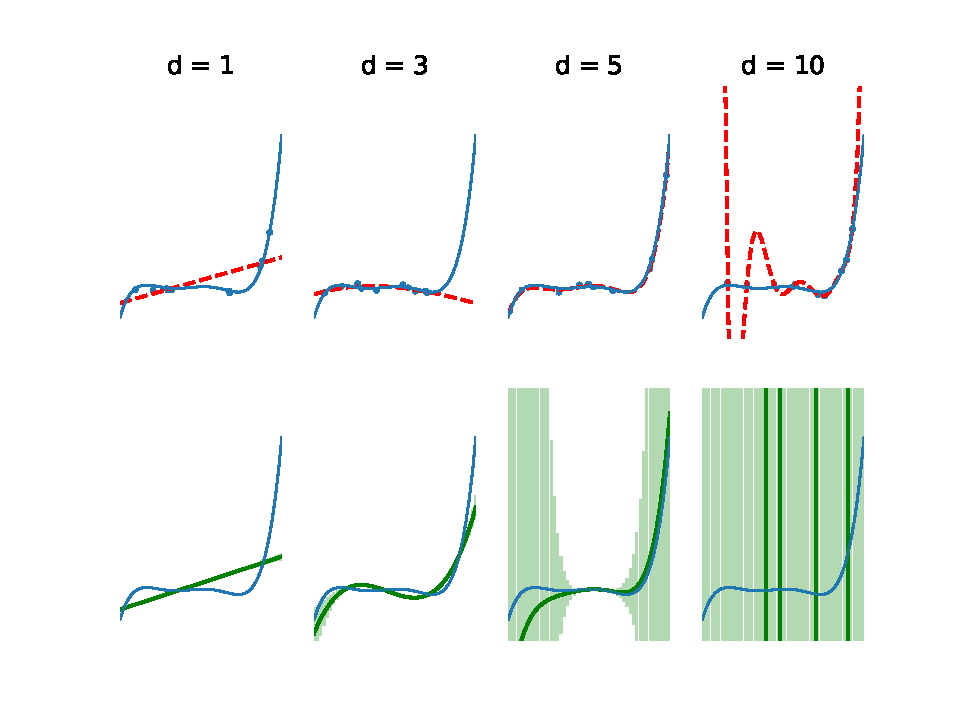
\includegraphics[width=0.49\linewidth]{graphics/poly_fit.pdf}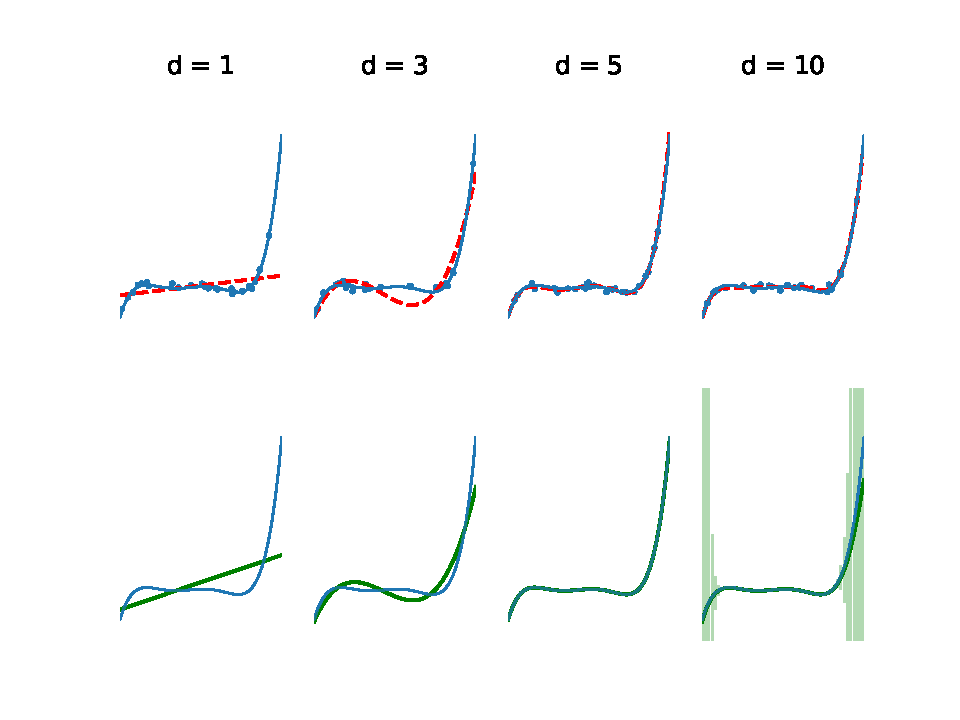
\includegraphics[width=0.49\linewidth]{graphics/poly_fit_large_n.pdf}
    \caption{Polynomial interpolation. Data is generated according to $y_i = p(x_i)+n_i$ for a degree five polynomial $p$ and noise $n_i$. An optimal polynomial of degree $d$ is inferred via empirical risk minimization with a least square loss. In the above plots, one learnt polynomial is shown, whereas the mean over 1000 instances together with errorbar corresponding to one standard deviation is show below. In the right plots, $10$ $x_i$ are drawn, and on the right, $25$ $x_i$ are drawn.}
    \label{fig:poly}
\end{figure}


\subsection{Model evaluation and tuning}
How do we determine if a machine learning model is performing well? A first idea is to have a look at the training loss. This however only gives a very rough - if any -- idea of its quality. Indeed, there are many situations where the training loss can be driven to zero -- i.e. the model can be made to fit the training labels perfectly -- but the model is rubbish. Think for example about the task of fitting a polynomial of high degree to data. If the degree is too high compared to the number of training samples, we will be able to interpolate the training labels perfectly without issue -- but this polynomial will most likely be extremely 'squiggly' and hence be terrible. This phenomenon, where the model fits the training data perfectly but generalizes badly to unseen data, is known as \textbf{overfitting}. 

Looking at the test loss can hence only detect that we are not \textbf{underfitting}, i.e. not adapting enough to the training data $(x_i,y_i)$.  What we ultimately is interested is how well the model can \textbf{generalize} to unseen examples. The correct way of determining which out of two machine learning models perform better is thus to compare their \emph{expected risks}. Remember that for a reasonable loss function, a lower risk means a better fit. However, given a fixed set of training data, the expected risk cannot be cannot be calculated! We see that by looking at its definition:
\begin{align*}
    \text{Expected risk} = \mathbb{E}_{D,x,y} \ell(f_D(x),y)
\end{align*}
We here take expected values both with respect to different draws of the training data $D$ -- but we only have one draw -- and also over unseen data $(x,y)$ -- which we do not access to. How should we solve this problem?

A first, obvious strategy is to split the available data into two sets: One set with which we do the training (a training set) $D_{\mathrm{tr}}$ and one set which we measure the error with (a \textbf{validation set}) $D_{\mathrm{val}}$. Since we imagine that all samples in the original data have been drawn independently, the validation error 
\begin{align*}
    CV = \frac{1}{\abs{D_\mathrm{val}}} \sum_{(x,y) \in D_\mathrm{val}} \ell(y,f_{D_\tr}(x))
\end{align*}
will be a (rough) estimate of the expected risk. Note that this strategy is very simple to implement -- and model agnostic.

\subsubsection{Test set vs. validation set} In the machine learning research community, it is common practice to make split into a training set and validation set once, and then always use the error on that validation set to compare different methods. Such a validation set is called a test set. This has pros and cons: agreeing on one common test set eliminates the element of chance when comparing methods. On the other hand, because a low test risk now in itself becomes a 'quality measure' of a research project, a lot of energy will be spent on making the model perform well on the specific examples decided upon as the 'true' test set. 

Importantly, a test set used to measure the quality \textbf{must not} be used to fine-tune the model (for example -- choosing the degree of the polynomial to use for polynomial interpolation) to obtain a better test score. If we do that we 'indirectly' let the machine learning model see the un-seen examples, which goes against the entire idea of generalization. Do not trust a stock-broker that can only show you that they can predict yesterday's stock prices!

Most machine learning methods have 'meta-parameters' that can be chosen freely. A (by now almost overused) example by us is the degree of the polynomials in a polynomial regression (we will get to know other examples of such metaparameters later). Choosing the meta-parameters to optimize performance is referred to as \textbf{tuning} the model. When using data to tune the model, one should hence \textbf{never} use the test set. Instead, one should use a separate subset of the training data to estimate the test error. This set is often referred to as a \textbf{validation set}. 

\subsubsection{Cross validation} Only using one set of observations as a validation set has two problems. First, we 'sacrifice' a part of the training data when we do not use it for training -- if we want a good estimate of the test error, that can be a significant part of the available data. Secondly, there is a high element of chance when drawing the validation set -- think for example about the consequences of drawing a validation set containing an outlier.

A more stable and sensible approach is to use so-called \emph{cross-validation}. Here, one divides the available data into $k$ equal parts $D_i$, and then train the model using all but one part, say $\hat{D}_{i} = D \backslash D_i$ $k$-times, measuring the error with the left-out data set each time. The cross-validation estimate of the training loss is then
\begin{align*}
    \frac{1}{k} \sum_{i\in [k]} CV_i = \frac{1}{k}\sum_{i \in [k]} \frac{1}{\abs{D_i}} \sum_{(x,y) \in D_i} \ell(y_i, f_{\widehat{D}_i}(x_i)).
\end{align*}
$CV_i$ hence denotes the validation loss when using $D_i$ as a validation set and $\hat{D}_{i}$ as a training set. 

The number $k$ of splits is free to choose, and its choice often boils down to practicality. The extreme case of using $k=n$, i.e. using validation sets of size $1$, called leave-one-out-training, could in principle be used. This would however be very expensive -- note that $k$-fold cross-validation requires us to repeat the training procedure $k$ times. Also, the smaller the $D_i$, the higher the overlap of the $\hat{D}_i$, leading to more correlated $CV_i$, leading to a worse estimate of the validation error. In practice, $k$ is  often chosen equal to either $5$ or $10$, since it empirically has been observed to give good estimates of the test error (on simulated data sets) while also not require too much extra training time.

\subsubsection{Bootstrapping} A technique similar to cross validation in spirit, but used for slightly different purposes is so-called \emph{bootstrapping}. Here, one would like to obtain an understanding of the distribution of a parameter of a model depends on the training set -- that could be the test error, but it could also be e.g. a regression coefficient of a (non)-linear model. E.g. the variance of that distribution can in very special cases -- typically after making assumptions on the nature of the training data and noise -- can sometimes be determined theoretically, but for more complicated models, this is hard. 

One therefore needs to resort to empirically determine the distribution -- i.e., redo the training with different training sets and record what happens. Since one only has one training set, one needs to 'pull oneself up by the bootstraps' to get new ones. What this means is that new training sets are 'simulated' via drawing subsamples of the training sets. One can then repeat the training for each such 'bootstrapped' training set, measure the metric of interest each time, and then obtain information about the distribution of it. In bootstrapping, in contrast to cross-validation, one draws the training sets with rather than without replacement. This means that the training sets are correlated, so that the obtained distribution only is an approximation of the one obtained for truly independent draws of the training set.

\subsection{Recommended reading and exercises}
Chapter 2 of \href{https://www.statlearning.com/}{An introduction to Statistical Learning} gives a good overview of the main ideas of statistical learning. Chapter 5 is about validation methods and boot strapping. If you need a refresher on linear regression, which we will continue to use as an example, it can be good to have a look at Chapter 3.

Good exercises from the textbook are 2.4.1-3 and 5.4.2-4. Make sure to take your time to properly reason about the concepts when solving the exercises. For practical exercises, see the Canvas webpage.


\section{Regularization}

The name of this course is statistical learning \emph{in high dimensions}. This refers to the setting when the number of features $p$ is high compared to the number of observations. This is not the setting of traditional statistics, but is nowadays very common in the wild:
\begin{itemize}
    \item Online retailers keep track of which products their customers buy. It is not uncommon for such retailers to have thousands of articles in stock. 
    \item In omics data (genomics, proteomics), hundreds of thousands of gene or protein expression data are recorded to diagnose illnesses. The number of patients in a typical study is typically much much lower.
    \item An image of resolution $B\times H$ pixels can be seen as a collection of $B\cdot H$ real-valued features. With $B$ and $H$ not uncommon to be in the thousands, we already have millions of features. Putting them next to each other to form a video could easily make them surpass a billion.
\end{itemize}
Having many features inevitably leads to a high computational burden. With computers becoming more and more powerful by the day, that is however \textbf{not} the main problem with doing statistics in high dimension. That is instead that they, \emph{without thought}, will be \emph{too flexible and very prone to overfitting}.

Let us formally explain the fundamental problem of high-dimensional statistics by taking a look at the familiar example of \emph{linear regression}. We remember the setting: We are given data $x_i \in \R^p$ and try to predict a response $y_i\in \R$ using a linear model $f(x)= a+ \sprod{\beta,x}$ for some $a\in \R$, $\beta \in \R^p$. To make the notational effort smaller, let us actually only write $f(x)=\sprod{\beta,x}$ -- by attaching a dummy feature with the value $1$ to all data-points $x_i$, we can still include an intercept. The empirical risk minimization problem with square loss, or MSE estimate (minimal least squares) of the parameters $\beta$ is then given by solution of
\begin{align}
    \min_{\beta \in \R^p} \tfrac{1}{2}\norm{X\beta-Y}_2^2. \label{eq:linreg}
\end{align}
In the high-dimensional setting, the number of observations $n$ is smaller than $p$, which means that $X$ is a 'short fat matrix'. It will therefore have  a non-trivial kernel, making the above problem \textbf{ill-posed}: It will \emph{always} have infinitely many solutions. Also, unless the data is 'degenerate', the matrix $X$ will have full rank, meaning that there \emph{always} exists \textbf{infinitely} many $\beta$ with $Y=X\beta$. 

How should we know which one of them to pick? If we simply choose one 'at random', the variance becomes infinite, which we by the 'fundamental theorem of statistical learning' means that the generalization will be rubbish.

We will encounter three 'approaches' to \textbf{regularizing} such ill-posed problems.
\begin{enumerate}
    \item \emph{Penalization} Add an extra term (penalty) to the empirical risk minimization to 'penalize' some 'bad behaviour' of the estimator $f$.
    \item \emph{Dimensionality reduction} Reduce the number of 'active features' in the dataset to turn it into a non-high-dimensional problem after all.
    \item \emph{Implicit regularization} Some methods work 'although they should not' due to mathematical properties of them working in our favor. This subtle phenomenon is referred to as 'implicit regularization'. It is hence not an 'approach' we can apply at will for any given method, but rather a phenomenon we that is there that we can take advantage of. We will point to it when we see it rather than chase it!
\end{enumerate}

\subsection{Ridge regression -- the simplest penalization strategy}
As we already have explained, the ERM \eqref{eq:linreg} will have an entire subspace of optimal solutions in the high-dimensional case $n>p$, and hence theoretically have infinite variance. A simple way to make the variance finite is to only allow for $\beta$ with small $\ell_2$-norm, the variance is at least finite. Instead of constraining the solution, we may instead \emph{penalize} large coefficent vectors $\beta$ with the help of an  $\ell_2$-norm \textbf{regularization} term;
\begin{align}
    \min_{\beta \in \R^p} \tfrac{1}{2}\norm{X\beta-Y}_2^2 + \lambda \norm{\beta}_2^2. \label{eq:ridgeregression}
\end{align}
Here, $\lambda>0$ is a (tuneable) meta-parameter. This problem is referred to  as \emph{ridge regression}.

In contrast to the unconstrained MSE, the ridge regression problem has a unique solution.

\paragraph{Remark} In practice, one does not penalize the coefficient related to the intercept - let us not show this in the notation for simplicity.

\begin{lemma}
    Problem \ref{eq:ridgeregression} has a unique solution for every $\lambda>0$, given by the following linear system of equations
    \begin{align}
        (\lambda \id + X^*X)\beta = X^*Y \label{eq:ridgesol}
    \end{align}
\end{lemma}
\begin{proof} The function $R_e(\beta)$ that we optimize in \eqref{eq:ridgeregression} is convex in $\beta$, meaning that the global minimum is characterized by a zero derivative. We have
\begin{align*}
    \nabla R_e(\beta) = X^*(X\beta-Y) + \lambda \beta = 0 \, \Leftrightarrow \, (\lambda \id + X^*X)\beta = X^*Y
\end{align*}
Now note that $X^*X$ is positive semi-definite, and thus only have non-negative eigenvalues $\sigma_i^2$. Consequently, the eigenvalues $\lambda + \sigma_i^2$ of $(\lambda\id + X^*X)$ are all positive, and hence, $\lambda \id + X^*X$ is a square matrix of full rank -- i.e., invertible.
\end{proof}

\paragraph{Remark} The etymology of 'ridge regression' is a bit complicated. Its origins can be traced in so-called \emph{ridge analysis}, which  is about determining minima and maxima of quadratic functions on circles centered around the origin. Solving such problems leads to equations of the form \eqref{eq:ridgesol}. As the radius of said circle changes, the maximum and minimum move along 'ridges' in the optimization landscape of the quadratic function, hence the name. \cite{hoerl2020ridge}

In order to get an idea of the impact of the $\lambda$ parameter, let us analyse what happens when $\lambda\to 0$ (low regularization limit) and $\lambda \to \infty$ (high regularization limit).

\begin{prop}
    Let $\beta_\lambda$ denote the solution of \eqref{eq:ridgesol}. Assume that $X$ has full rank. Then
    \begin{itemize}
        \item $\lim_{\lambda \to \infty} \beta_\lambda = 0$
        \item  Let $\beta_0$ denote the solution to $X\beta =Y$ with minimal $\ell_2$-norm. Then, $\lim_{\lambda \to 0^+} \beta_\lambda=\beta_0$
    \end{itemize}
\end{prop}

We skip this proof in the lecture - we will get back to it when we talk about other types of regularized linear regression at the end of the course. 

\begin{proof} 

    We know that we make a singular value decomposition of the matrix $X$: $X = U\Sigma V^*$ for $U \in \R^{n,n}$, $V\in \R^{p,p}$ orthogonal, and $\Sigma = [\Sigma_0 \, 0]\in \R^{n,p}$. (Remember that we are in a high dimensional setting, so that $n<p$). $\Sigma_0$ is a diagonal matrix with diagonal entries equal to the singular values of $X$. Now, $X\beta = Y$ can be written as
    \begin{align*}
        U \Sigma V^*\beta = Y \, \Leftrightarrow \Sigma V^*\beta = U^*Y.
    \end{align*}
    If we define $\gamma = V^*\beta$, and write $[\gamma_0 \, \gamma_1]^*$ with $\gamma_0 \in \R^n$ and $\gamma_1 \in \R^{p-n}$, we for one know that $\norm{\beta}_2^2 = \norm{\gamma}_2^2 = \norm{\gamma_0}^2_2 + \norm{\gamma_1}_2^2$ (orthogonality), and the above can be written
    \begin{align*}
        U^*Y = [\Sigma_0 \, 0 ][\gamma_0 \, \gamma_1]^* = \Sigma_0 \gamma_0.
    \end{align*}
    We see that in order to minimize the norm of $\gamma$ and still fulfill the above, we should choose $\gamma_1=0$ and $\gamma_0 = \Sigma_0^{-1}U^*Y$.

    Now let us have a look at \eqref{eq:ridgesol}. Note that 
\begin{align*}
    X^*X = V\Sigma^*U^*U \Sigma V^* = V  [\Sigma_0 \, 0] [\Sigma_0 \, 0]^* V^* = V\begin{bmatrix} \Sigma_0^2 & 0 \\ 0 & 0 \end{bmatrix} V^*.
\end{align*}
Therefore,  \eqref{eq:ridgesol} can be written
\begin{align*}
    V\begin{bmatrix} \lambda + \Sigma_0^2 & 0 \\ 0 & \lambda \end{bmatrix} V^*\beta = V\begin{bmatrix} \Sigma_0 \\ 0 \end{bmatrix} U^*Y
\end{align*}
Here, we used that $V$ is orthogonal, so that $\id = VV^^*$. Now, let us again write $V^* \beta = [\gamma_0 \, \gamma_1]^*$. Then, the above reduces to 
    \begin{align*}
        \begin{bmatrix} (\lambda + \Sigma_0^2) \gamma_0 \\ \lambda \gamma_1 \end{bmatrix} = \begin{bmatrix}
            \Sigma_0 U^*Y \\ 0 
        \end{bmatrix},
    \end{align*} 
    so that $\gamma_1 = 0$ and $\gamma_0 = (\lambda + \Sigma_0^2)^{-1}\Sigma U^*Y$. Now notice that both $\lambda + \Sigma_0^2$ and $\Sigma_0$ are diagonal. The diagonal elements are given by
    \begin{align*}
        ((\lambda + \Sigma_0^2)^{-1}\Sigma_0)_{ii} = \frac{\sigma_i}{\lambda +\sigma_i^2}.
    \end{align*}
    This goes to $\sigma_i^{-1}=(\Sigma_0^{-1})_{ii}$ when $\lambda\to 0^+$ and to $0$ for $\lambda \to \infty$. This proves the claim.

\end{proof}

Let us now interpret this proposition.

\paragraph{High regularization} When \textbf{$\lambda$ is very high}, ridge regression will \emph{for any data} put out a $\beta$ close to zero.  It will thus change much for different draws of the data, so that the \textbf{variance is low}. On the other hand, for most ground truths, $\beta\approx 0$ will be a bad estimator, so that the \textbf{bias is high}.

\paragraph{Low regularization} For \textbf{$\lambda$ very small} $\beta$ will be very close to the minimal $\ell_2$-norm solution of $X\beta = Y$. This object behaves in a more complicated manner on $X$, and it is therefore a bit harder to analyze.

To be able to do it, let us assume that the ground truth assumption is perfect, i.e. that that there exists a $\beta_*$ with $y=\sprod{\beta_*,x}$ (no noise). Then, one can argue that the optimal solution $\beta_0$ of \eqref{eq:ridgeregression} will be equal to \emph{the projection of $\beta_*$ onto the orthogonal complement of the kernel of $X$}, which is the same as the span of the feature vectors $x_i$:
\begin{align*}
    \beta_0 = \text{Projection of $\beta_*$ onto $\mathrm{span}(x_i)$}
\end{align*}
We now note that 
for vectors $\tilde{x}$ in $\mathrm{span}(x_i)$,  $\sprod{\beta_0,\tilde{x}}= \sprod{\beta_*,\tilde{x}}$, i.e., the classifications will be correct. If instead $\tilde{x}$ lies outside $\mathrm{span}(x_i)$, the classifications will be wrong. Hence, \textbf{if it is probable that unseen data points lie in the span of the training data, the bias will be low, otherwise not}. 

Whether that is true depends highly on the data-distribution. If the span of all datapoints $x \in \R^p$ are 'completely' random (e.g. if they are Gaussian distributed), unseen data is usually not in the span of the training data: unless we have draw $n=p$ points, the ridge regression estimate will be biased. If we however all (training and test) data points $x$ lie in a (n unknown) $d$-dimensional subspace, and the vectors are reasonably distributed in there, already around $n=d$ training vectors will be enough to capture the span of all $x$.

As for the \textbf{variance}, one should remember that in realistic scenarios, the labels typically contains some random noise. This noise also needs to be fitted in the constraint $X\beta=Y$, which will induce some variance also in the coefficient vectors $\beta$. How big this variance is depends on the singular values of the matrix $X$, but it is typically non-zero. It is therefore likely that the optimal bias-variance tradeoff happens somewhere else than at $\lambda=0$. This optimal point should be sought for with the validation method discussed above -- for instance via cross-validation. 

A few more practical considerations.
\begin{itemize}
    \item Note that the scaling of the features will have an impact on ridge regression estimates. This is different than standard linear regression -- there, a scaling of a feature can easily be mitigated by scaling of the corresponding coefficient. In ridge regression, the rescaled coefficients will have a different error! It is therefore wise to scale the features so that they are all centered and have variance one.
    \item One should be very careful \text{ when interpreting} the ridge regression estimate  $\beta$. One cannot do it in the same way as in low-dimensional linear regression. In particular, we have seen that even in the low bias setting of $\lambda\to 0^+$, the returned coefficient vector is not the ground truth $\beta_*$, but rather a projection of it to the span of the training data. This may, as we have seen, still yield good test risks, but may be a completely different vector! One should hence be careful drawing conclusions about which features are important, for instance, from looking at $\beta_\lambda$.
\end{itemize}

\subsection{Feature selection}
As we have seen, the fundamental problem of linear regression in high dimension is that there are two many features that can be fitted. In many settings, there is a reason to believe that there exists a \emph{subset of the features} which are enough to explain the output variable, and that the rest of the simply distractors. To find such a subset would also help interpretation -- if we for instance can find a few genes in a genomic dataset that in themselves predict a certain diagnosis, that could help us better understand the illness.

If a sparse solution exists, knowing its support is a very powerful regularizer to perform regression. If we would know a priori which features are important, we could simply perform a linear regression from those features. If $s$ features are 'active', we then only need to estimate $s$ coefficients in $\beta.$
This strategy is hence a form of \textbf{dimension reduction}.

Now, how does one find which features which are important? The most straightforward way of finding a sparse explanatory variable is to simply go through all subsets of features, perform linear regression, evaluate the estimates, and select the best one, using a carefully chosen metric. The naive approach of simply going through all subsets will require us, if $p$ features are available, to perform $2^p$ linear regressions. Already for $p\approx 20$, that amounts to more than a million problems! 


One clearly needs to proceed a bit more carefully. A canonical heuristic is \emph{forward selection}. In that setting, we start with zero variables, and test all the $p$ models with one active feature, and the one with the smallest training error is chosen. From there, we test the $(p-1)$ models that result from adding one more feature, select the best one, and so on. Backward selection does the opposite -- then we start with all variables, and remove one variable at a time. This will make us only test $p + (p-1)+(p-2) + \dots = \frac{p(p-1)}{2}$ subsets, which already is much better (we can of course also stop earlier using some criterion). Still, if $p$ is very high, this may still be far too expensive. Also, if $p>n$, backward selection will without regularization in the early iterations give us the same training error for all subsets, since they all will be able to perfectly fit the data.





\subsection{Principal Component Analysis}
In feature selections, we assume that a small numbers of the features $x(k)$ are important. This is great for interpretability, but if good estimation is key, who says we cannot build more complicated 'dimension-reduced' features? One can take linear combinations like this:
\begin{align*}
    z(k) = \sprod{\phi_k , x} = \sum_i \phi_k(i)x(i)
\end{align*}
How should the $\phi_k$ be designed to optimally 'capture' the information in the data? 

To understand this, we can again use intuition from linear algebra: When recording $\sprod{\phi_k,x}$, we disregard any information in the orthogonal complement of the $\phi_k$. We should hence try to let the $\phi_k$ \text{span a subspace which approximates the data $x$ as well as possible.} Mathematically: given a distribution of the data $x_i \in \R^p$, what is, for a given $r$, the $r$-dimensional (affine) subspace $\calU$ that best approximates the data, in the sense of minimizing the expected squared distance to the subspace
\begin{align*}
    \mathbb{E}(\dist(x,\calU)^2)?
\end{align*}

The solution to this problem is given by the following theorem:

\begin{theorem} \label{th:svd}
   An $r$-dimensional subspace $\calU = \{U\rho+b, \rho \in \R^r\}$ minimizes the expected distance from the data vector $x$ to $\calU$ if and only if the orthogonal columns $U^i \in \R^p$ of $U$ are the orthogonal directions $\phi_0, \dots, \phi_{r-1}$ that maximizes the variance
   \begin{align} \label{eq:maxvar}
       \sum_{i \in [r]} \mathbb{V}(\sprod{\phi_i,x})
   \end{align}
   among all such $r$-tuples of directions.

   The $\phi_k$ can be determined via a singular value decomposition: Let $\overline{x}=x-\erw(x)$ be the normalized data, and define
   \begin{align*}
       M = \erw(\overline{x}\overline{x}^*).
   \end{align*}
    Then, the $\phi_k$ are the $r$ first columns of the matrix $\Psi$ in the singular value decomposition $M = \Psi \Sigma \Psi^*$
\end{theorem}

The proof of this theorem is rather technical and does not provide much insight - we skip it in the lecture.

\begin{proof}
Let us introduce some notation. An $r$-dimensional affine subspace has the form
\begin{align*}
    U\rho + b, \rho\in \R^r 
\end{align*}
for some $b\in\R^p$, $U\in \R^{p,r}$ with orthonormal columns. In this notation,
\begin{align*}
    \dist(x,\calU)^2 = \min_\rho \norm{x-(U\rho+b)}^2 =  \min_\rho \norm{x-b}^2 - 2\sprod{x-b,U\rho} + \norm{\rho}_2^2,
\end{align*}
where the final step follows from the fact that $U$ has orthonormal columns.
For a fixed $x$, that  minimizer is simple to calculate -- it is characterized by
\begin{align} \label{eq:scores}
    \rho-U^*(x-b)=0.
\end{align}
Putting this into our formula for $\dist(x,\calU)$ yields
\begin{align*}
   \dist(x,\calU)^2 = \norm{x-b -UU^*(x-b)}_2^2 = \norm{(\id-UU^*)(x-b)}_2^2. 
\end{align*}
We are interested in the $b$ and $U$ which minimizes
\begin{align*}
    \mathbb{E}(\dist(x,\calU)^2) = \mathbb{E}(\norm{(\id-UU^*)(x-b)}^2)
\end{align*}
get minimal? If we write $\id-UU^*=P$, it is simple to determine the optimal $b$ for a given $P$-- taking the derivative, we obtain that the optimal $b$ is characterized by
\begin{align*}
    \mathbb{E}(P^*P(x-b))=P^*P(\mathbb{E}(x)-b)
\end{align*}
We see that putting $b = \mathbb{E}(x)$ always does the job. Let us introduce the notation $\overline{x}$ for the normalized features $x- \mathbb{E}(x)$. We will now prove the formula 
\begin{align} \label{eq:minmax}
    \erw(\norm{(\id-UU^*)\overline{x}})_2 = \mathbb{V}(x) - \mathbb{V}(U^*x)
\end{align}
Since $\mathbb{V}(x)$ is a constant only dependent on the data, this shows that the distance to the subspace is minimized exactly when $\mathbb{V}(U^*x) = \sum_{i \in [r]}\mathbb{V}(\sprod{\phi_i,x})$ is maximal. This is the first claim.

So let us prove \ref{eq:minmax}.  We have
\begin{align*}
    \norm{(\id-UU^*)\overline{x}}_2^2 = \norm{\overline{x}}_2-2\sprod{UU^*\overline{x},x} + \sprod{UU^*\overline{x},UU^*\overline{x}}.
\end{align*}
Now, $\sprod{UU^*\overline{x},UU^*\overline{x}} = \sprod{UU^*\overline{x},\overline{x}}$. This can be seen by noticing that since $U$ has orthogonal columns, $U^*U=\id$, so that
\begin{align*}
\sprod{UU^*\overline{x},UU^*\overline{x}} = \sprod{UU^*UU^*\overline{x},\overline{x}} = \sprod{UU^*\overline{x},\overline{x}}.
\end{align*}
Anyhow, consequently,
\begin{align*}
    \erw(\norm{(\id-UU^*)\overline{x}})_2 = \erw(\norm{\overline{x}}^2 - \sprod{UU^*\overline{x},x})  = \erw(\norm{\overline{x}}^2- \norm{U^*\overline{x}}^2) = \mathbb{V}(x) - \mathbb{V}(U^*x),
\end{align*}
which was to be proven.

To prove the second claim is actually quite involved. Let us start by considering the case $r=1$: The variance of $\sprod{\phi,x}$ is equal to 
\begin{align*}
    \erw(\sprod{\phi, \overline{x}}^2) = \erw{\phi^*\overline{x}\overline{x}^*\phi} = \erw{\sprod{\phi,\overline{x}\overline{x}^*\phi}} = \sprod{\phi, M \phi}. = \sprod{\phi,\Psi\Sigma^2\Psi^*\phi} = \sprod{\Psi^*\phi,\Sigma^2\Psi^*\phi}.
\end{align*}
Since $\Psi$ is orthonormal, $\Psi^*\phi=\tilde{\phi}$  is also a direction of norm one. We now have
\begin{align*}
    \sprod{\Psi^*\phi,\Sigma^2\Psi^*\phi} = \sum_{k\in [p]} \sigma_k^2\tilde{\phi}(k)^2.
\end{align*}
We see that this is smaller than $\sigma_0^2$, since $\sum_{k\in [\pi} \sigma_k^2\tilde{\phi}(k)^2=1$. However, we also obtain that value by putting $\tilde{\phi}(0)=1$, and the rest $0$. Hence, the maximum is given by $\sigma_0^2$, and it is obtained for $\tilde{\phi}=e_0$, i.e $\phi = \Psi \tilde{\phi} = \Psi e_0$ the first column of $\Psi$.

To get the general statement, notice that we are looking for the $\phi_i$ which maximize
\begin{align*}
    \sum_i \sprod{\phi_i,M\phi_i}.
\end{align*}
It is clear by the above argument that choosing $\phi_i$ equal to the $i$:th singular vector of $M$, we can get this value equal to $\sum_{i< r}\sigma_i^2$. We hence need to show that the value is not bigger for any other choice. We do this via induction over $r$ using an argument from argument from \cite{tao2012topics}. The case $r=1$ is already treated. To go from $r$ to $r+1$, consider the restriction $N$ of $M$ on the orthogonal complement of the first singular vector $\psi_0$. This operator has singular values (eigenvalues) $\sigma_1^2, \dots, \sigma_{n-1}^2$, so that by induction, we have
\begin{align*}
     \sum_{i\in [r]} \sprod{\phi_i,N\phi_i} \leq \sum_{i=1}^r \sigma_i^2
\end{align*}
for all $r$-tuples of orthonormal vectors $\phi_i$. Since the final scalar product is bounded above by $\sigma_0^2$ by the case $r=1$, the claim follows for $r+1$.
\end{proof}

The theorem provides a nice connection between geometry and statistic: In order to approximate the data by a lower-dimensional subspace, we should try to find the direction in which the data varies as much as possible (one often says that the directions \emph{explain} a part of the variance). 


The $\phi$ maximizing $\eqref{eq:maxvar}$ are called the \emph{principial components} of the data. In practice, we of course do not have access to the actual expected value of $\erw{\overline{x}\overline{x}^*}$, but we can use the empirical covariance instead:
\begin{align*}
  \tilde{M} = \frac{1}{n-1} \sum_{k\in [n]} (x_k - \mu)(x_k-\mu)^*, \quad  \mu(x) = \tfrac{1}{n} \sum_{k \in [n]} x_k.
\end{align*}
(The $(n-1)$ in the denominator is to make the estimate unbiased). The singular vectors (or rather eigenvectors) of these matrix are often referred to as the principial components of the data matrix $X$, although they technically are rather are empirical estimates of the 'true' principial components of the data.

The feature $z(k)=\sprod{\phi_k,x}$ is called the \emph{score} of the $k$:th principial component. Note that the scores are uncorrelated:
\begin{align*}
    \mathrm{Cov}(z(k),z(\ell)) = \mathbb{E}(\sprod{\phi_k,\overline{x}}\sprod{\overline{x},\phi_\ell}) = \sprod{\phi_k,M\phi_\ell} = \sigma_\ell^2 \sprod{\phi_k,\phi_\ell}=0, \quad k\neq \ell
\end{align*}

\paragraph{Example} The \texttt{sklearn}-package for python contains a lot of functionality for statistical learning, and also a few toy datasets. One of them is a dataset consisting of 1797 $8\times 8$ images of handwritten digits. Note that we can alternatively view these as $\R^{64}$-vectors, and thus perform a PCA. In Figure \ref{fig:digits_components}, we show the first $8$ principial components to the left, and a so-called \emph{scree plot} on the right. A scree plot is a plot on how the \emph{relative explained variance} $\frac{\mathbb{V}\sprod{\phi_k,x}}{\mathbb{V}(x)}$ depends on the component number $k$. We see that from component $30$ or so onwards, the new directions only explain about $1\%$ of the variance. In other datasets, this may be even more extreme. It is a good approximation to use as many components as is needed for the scree plot to stop falling of quickly -- in a more serious downstream application, we should of course use the techniques we presented in the first lecture instead to tune the number of components.

A more striking showcase that the first few principial components is enough to capture the gist of the data is Figure \label{fig:digits_approx}. Here, we take an image from the dataset (viewed in the right-most plot) and plot the best approximations $\sum_{i\leq r} \sprod{\phi_i,x}\phi_i$ of the images using $1$, $2$, $5$ and $10$ principial components. We see that already $5$ components is enough to recognize the image as a '5'.

In Figure \ref{fig:digits_cluster}, we plot the first two score features $z_i =\sprod{\phi_i,x}$ for the entire dataset. We see that the images are naturally 'clustured' according to its label. Such score scatter plots is a nice and intuitive way of visualizing datasets, and shows that already the first scores can be used to differentiate between classes. We will towards the end of the course learn more about clustering methods, but let us already now record that performing the clustering on a dimensionality-reduced version of the dataset may be a good idea.

\begin{figure}
    \centering
    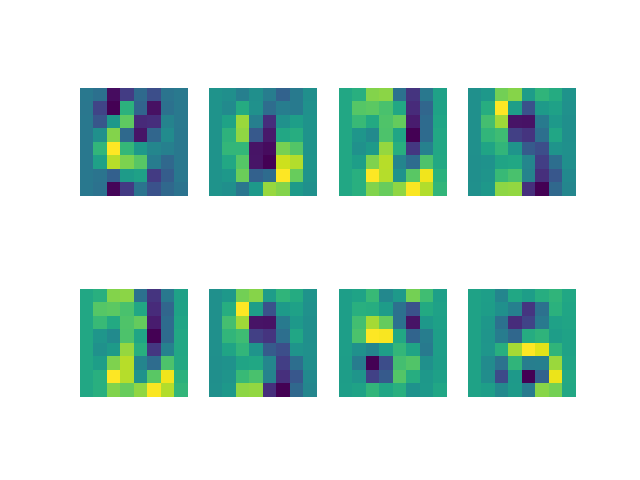
\includegraphics[width=.54\linewidth]{graphics/digits_components.png}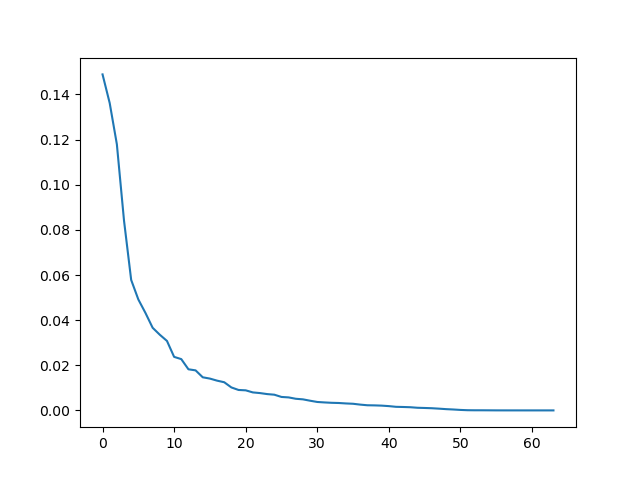
\includegraphics[width=.45\linewidth]{graphics/digits_scree.png}
    \caption{(Left) The first $8$ principial components for the \texttt{digits} dataset. (Right) Scree plot}
    \label{fig:digits_components}
\end{figure}


\begin{figure}
    \centering
    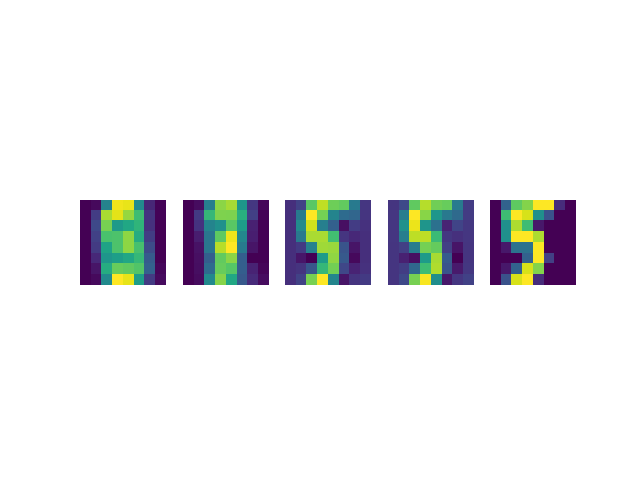
\includegraphics[width=.75\linewidth]{graphics/digits_approximations.png}
    \caption{An image approximated with the help of $1$, $2$, $5$ and $10$ first principial components - the original image is to the right.}
    \label{fig:digits_approx}
\end{figure}


\begin{figure}
    \centering
    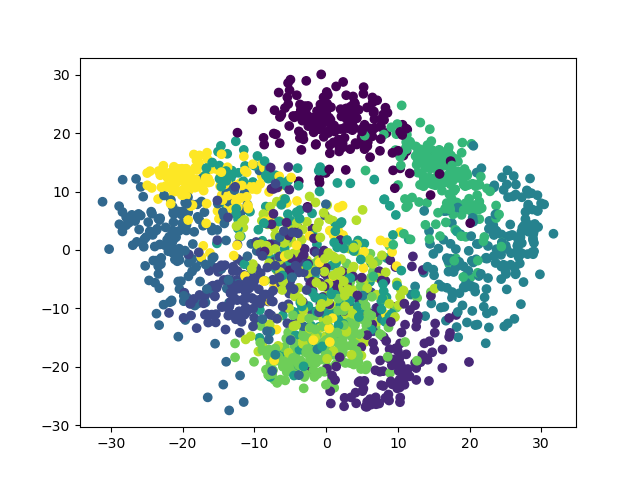
\includegraphics[width=.75\linewidth]{graphics/digits_clustering.png}
    \caption{A scatter plot of the first two score features of the \texttt{digits dataset}.}
    \label{fig:digits_cluster}
\end{figure}



%\paragraph{Example: PCR} PCR is short for \emph{principial component regression}. The principle behind this method %is simple: instead of regressing $y$ from the features in $x \in \R^p$ directly, one first calculates the %principal components of $X$, forms the score vectors $z_k$, and solves the regression problem
%\begin{align*}
%    \min_{\beta\in \R^r} \tfrac{1}{2}\norm{Z\beta - Y}_2^2
%\end{align*}
%Any other method we come across in this course can be applied to such dimension-reduced features!

%\subsection{Clustering with PCA} The principial components can be used for very simple \emph{clustering} of the %data. To explain this, let us first assume that $p=2$. We can then examine the data by a simple scatter plot. We %have done this for a simulated data set in Figure (\ref{fig:clusters1}). The data was  obtained via -- with equal %probability -- drawing points from two Gaussians with different means (one speaks of a \emph{mixture} of two %Gaussians. It is not hard to see that the data can be divided into two classes depending on which Gaussian it was %drawn from.

%\begin{figure}
   % \centering
   % 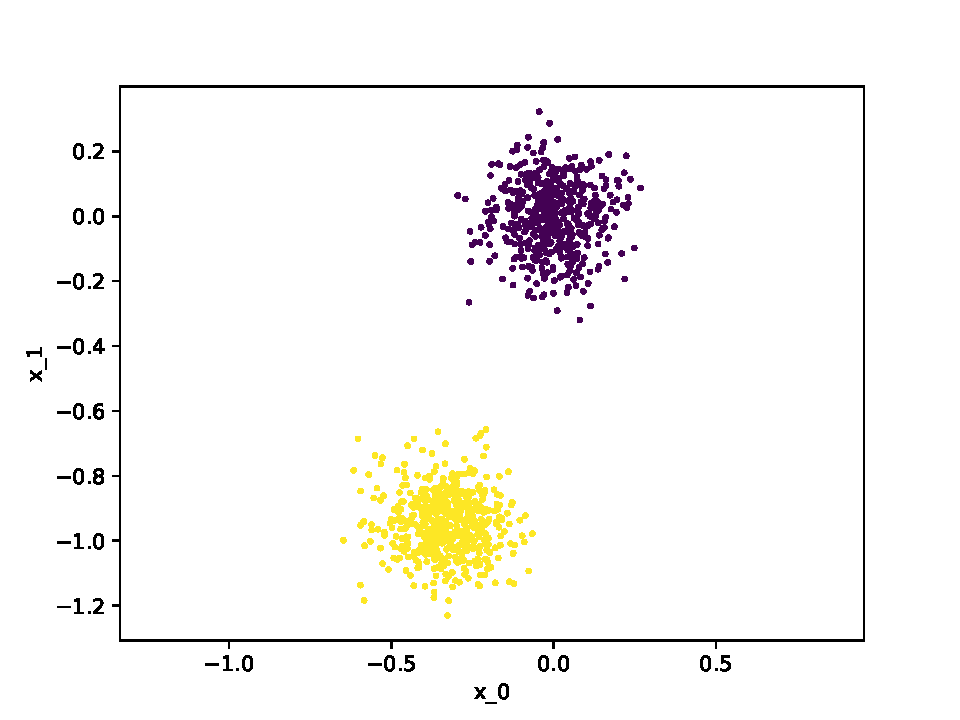
\includegraphics[width=0.5\linewidth]{graphics/2_feature_clusters.pdf} 
  %  \caption{A mixture of two Gaussians of dimension $2$. Best viewed in color.}
 %   \label{fig:clusters1}
%\end{figure}

%\begin{figure}
  %  \centering
 %   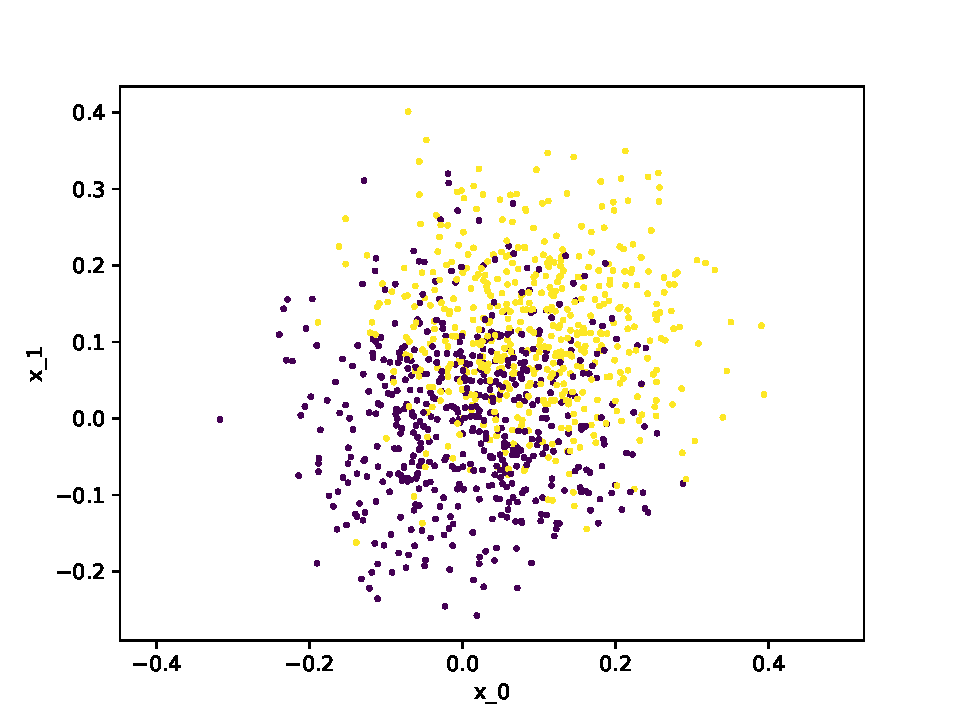
\includegraphics[width=.45\linewidth]{graphics/100_feature_clusters.pdf}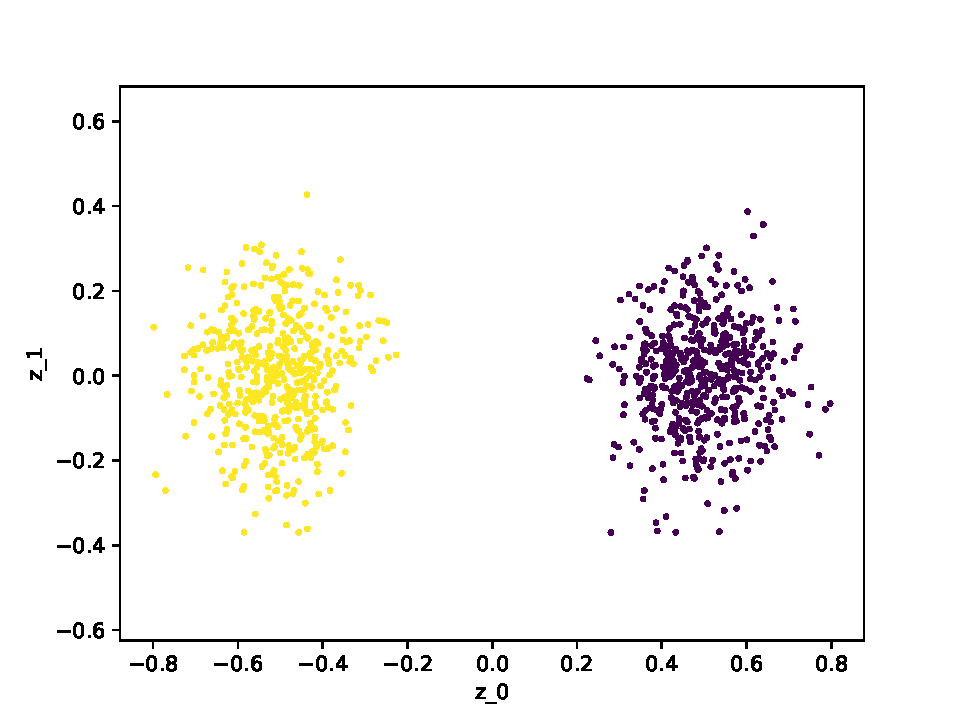
\includegraphics[width=.45\linewidth]{graphics/100_feature_clusters_pca.pdf}
%    \caption{Left: A scatter plot of two features $x_0$, $x_1$ for a mixture of two Gaussians in dimension %$p=100$. Right: The PCA scores for the same data. Best viewed in color.}
 %   \label{fig:clusters}
%\end{figure}


%Can we do something similar when $p>2$? One can of course choose two features and make scatter plots. It is however hard to know which two features to choose -- there are $p(p-1)/2$ pairs to choose from -- and none of them need to be very informative. In Figure \ref{fig:clusters}, we have made such a plot for feature vectors $x\in \R^{100}$ drawn from a synthetic dataset constructed similarly as in the former case. We see that the clusters no longer can be determined visually. 

%If we however calculate the principial components and make a scatter plot of the scores along the first two of them, the clusters emerge again! Since the principial components are directions of high variance, such important variances as difference between two clusters may be revealed in such a plot. (If the inter-cluster variances are too big, this will probably not suffice). We will return to more sophisticated means of clustering later.

%\subsection{PCA and low-rank approximation}
 %What the PCA implicitly does is finding a subspace that fits the data well. More exactly, when solving the empirical version, we are finding a subspace $\calU$ that solves the problem
 %\begin{align*}
 %    \min_{\calU} \frac{1}{n}\sum_{k \in [n]} \dist(x_k,\calU^2) &= \min_{U\in \R^{p,r},b \in \R^p,\rho_k \in \R^r} \frac{1}{n} \sum_{k \in [n]} \norm{U\rho_k+b-x_k}^2_2 \text{ subject to columns of } U \text{ orthonormal} \\
 %    &= \min_{U\in \R^{p,r},\rho_k\in \R^r} \frac{1}{n} \sum_{k \in [n]} \norm{U\rho_k- \overline{x}_k}^2_2 \text{ subject to columns of } U \text{ orthonormal}
 %\end{align*}
 %where the second step follows from the calculations above and the definition of the centered variables $\overline{x}_k = x_k - \tfrac{1}{n}\sum_{k\in [n]} x_k$. Now let us rewrite this slightly: If we let $Z \in \R^{n,r}$ be the matrix with $k$:th row $\rho_k$, $U\rho_k$ is the $k$:th row of $ZU^*$. The notation $Z$ is explain by \eqref{eq:scores} -- by that equation, $\rho_k=U^*{x}_k$, and $U^*\overline{x}_k$ is simply the vector of scores for the $k$:th observation in the case of centered variables.
 
% The above sum is then the sum of the norms of the rows of the matrix $ZU^*-X$, i.e the difference of $ZU^*$ and $X$ in \emph{Frobenius norm}.
% \begin{align*}
 %    \min_{U \in \R^{p,r}, Z\in \R^{n,r}} \tfrac{1}{n}\norm{ZU^*-\overline{X}}_F^2
 %\end{align*}
 %A matrix in $\R^{n,p}$ can be written as $ZU^*$ if and only if it has rank smaller than $r$. Solving the PCA problem is \emph{implicitly} finding the matrix of \emph{low rank} that best approximates the centered data matrix $\overline{X}$!
 %\begin{align*}
%     \min_{L \in \R^{n,p}} \norm{L-\overline{X}}_F^2 \text{ subject to $\mathrm{rank}(L)\leq k$.}
% \end{align*}
 %If the PCA can explain a lot of the variance means that $\overline{X}$ can be well approximated by a matrix of low rank. This is empirically true for many data sets. Assuming this is an interesting assumption that can be leveraged for many tasks.
 %An example is the problem of \emph{matrix completion}, or \emph{missing observations}. Here, we assume that we only have access to $x_i(j)$ for a subset $\Omega$ of all pairs $(i,j)$. An illustrative example is the one of recommender systems on streaming platforms. Here, the observations $x_i(j)$ is the score the $i$:th user gives the $j$:th movie/series. Most users have only seen a few movies, so that $x_i(j)$ is unseen for most $i$ and $j$. Can we find a low-rank matrix that explains the observations we have made?
 %\begin{align*}
  %  \text{ Find a low-rank matrix $L$ so that } X_{i,j} \approx L_{i,j} \text{ for } (i,j) \in \Omega
 %\end{align*}
 %Because of the streaming platform motivation, this problem is known as the \emph{Netflix problem}.

 %There is a plethora of methods for low-rank approximation, and a lot of theory of when they work. Let us not get into that, and let us instead note that we can use PCA to resolve the iterative approach outlined in Algorithm \ref{alg:LowRank} Here, we iteratively build a low-rank matrix $\Xi^{k+1/2}$ that approximates $X$ on the observed values.  

 %\begin{algorithm}[tb]      
%	\caption{Low rank approximation via alternating directions} 
%	\label{alg:LowRank}
%	\begin{algorithmic} [1]
% 		\REQUIRE Data matrix $X$,  set of observations $\Omega$
 %       \STATE Calculate the averages $\overline{x}_j$ of the observed values of feature $j$
 	%	\STATE $\Xi^0_{ij}=X_{ij}$ for $(i,j)\in \Omega$, $\Xi^0_{ij}=\overline{x}_j$ if $(i,j)\notin \Omega$.
 		%\REPEAT
 			%\STATE Determine the $U \in \R^{p,r}$ and $Z \in \R^{n,p}$ that minimizes
            %\begin{align*}
            %    r_k = \norm{\Xi^k-ZU^*}_F^2.
            %\end{align*}
%            That is: calculate principal components of $\Xi$ to get $U$, then set $Z$ to the scores of $\Xi^k$ for those components. Set $\Xi^{k+1/2}=ZU^*$
 %           \STATE Determine $\Xi^{k+1}$ as the solution of
  %          \begin{align*}
   %             \min_{\Xi \in \R^{n,p}}\norm{\Xi-\Xi^{k+1/2}}_F^2 \text{ subject to } \Xi_{i,j}=X_{i,j}, \ (i,j) \in \Omega
    %        \end{align*}
     %       That is, $\Xi^{k+1}_{i,j}=X_{i,j}$ for $(i,j)\in \Omega$, $\Xi^{k+1}_{i,j}=\Xi^{k+1/2}_{i,j}$ if $(i,j) \notin \Omega$.
 	%	\UNTIL $\sum_{i,j\in \Omega}(X_{i,j}-\Xi^{k+1/2}_{i,j})^2 $ small enough
 		%\RETURN Return $\Xi^{k+1/2}$
	%\end{algorithmic}
%\end{algorithm}

\subsection{Further reading}
PCA is discussed briefly in section 6.3.1 in Introduction to statistical learning, and more thoroughly in Section 12.2. 12.3 is specifically about missing values and matrix completion. Exercises in the statistical learning about PCA are 12.6 and the first half of 12.10 (this is a practical exercise, which can be better put into context after learning about $K$-means clustering -- which we will do later in this course).

Also consider the following exercises.

\begin{exercise}
    Assume that there is a noise-free, ground-truth linear relation hip between the labels $y \in \R$ and data-points $x\in\R^p$. Show that if the data distribution $x$ (i.e. both training and test-data) is contained in an $r<p$-dimensional subspace, applying PCR is equivalent to the low-regularization limit of ridge regression.  
\end{exercise}

\begin{exercise}
    Let $X\in \R^{n,p}$, with $n<p$, be a data matrix. Argue that the training samples $(x_i)_{i \in [n]}$ are always contained in an $n$-dimensional vector space. Does this imply that we in any learning task equally well can use the first $n$ scores $z(\ell)$ instead of the features $x(k)$?
\end{exercise}

\begin{exercise}
    In this exercise, we will explore the 'PCA'-clustering technique theoretically.

    \begin{enumerate}[(i)]
        \item Let $p$ be a $\mathrm{Ber}(\sfrac{1}{2})$ variable (i.e. a variable which is either zero or one, with equal probability), $z\in \R^p$ be a vector of i.i.d. $\calN(0,\sigma^2)$-distributed variables, and $\mu_0$ a non-zero vector in $\R^p$. Argue that the random variable
        \begin{align*}
            x = p\mu_0 + z
        \end{align*}
        is a simple model of a two-cluster dataset. (\emph{Hint}: What happens when $\mu_0$ is the first unit vector, and $p=2$?)
        \item Generate a dataset by sampling the above variable, perform a PCA and make a score scatter plot as in Figure \ref{fig:digits_cluster}. What do you notice?
        \item Show that the true covariance matrix $\erw{\overline{x}\overline{x}^*}$ will always have $\mu_0$ as a first two principial component. 
        \item With the help of (iii), explain the appearance of the figure you generated in (ii).
    \end{enumerate}
\end{exercise}


\section{Classical approaches to Classification}
Up until now, we have been mostly concerned with linear regression, i.e., explaining our output $y$ using a linear function $\sprod{\beta,x}$. Needless to say, it is in many cases extremely unlikely that that model will perfectly explain the data. A good example for this is \emph{classification problems}. Here, the response variable $y$ is binary. Examples:
\begin{itemize}
    \item $y=1$ if a patient is ill, $y=0$ if it is not.
    \item $y=1$ if an image depicts a dog, $y=0$ else.
    \item $y=1$ if a credit customer defaults, $y=0$ if they do not.
\end{itemize}
It is natural to also allow for multiple classes $\{0,\dots, k-1\}=[K]$ in classification problems -- we will describe how then can be handeled in each case, but in our general arguments, we will mostly focus on the binary case.

We can of course try to use a linear classifier $\sprod{x,\beta}$ to predict $y$. If the classifier returns a value between $0$ and $1$, we can interpret the value of the classifier as a probability. However, it is very likely that $\sprod{x,\beta}$ for some $x$ are smaller than $0$, and bigger than $1$ for others. How can then $\sprod{x,\beta}$ be interpreted? It is clear that this method is too naive.

Before getting to concrete methods, let us explain the concept of an \textbf{decision boundary} of a classifier. Note that every classifier function $f: X \to \{0,1\}$ will divide $X$ into two sets
\begin{align*}
    \mathds{0} = \{x \, \vert \,  f(x)=0\} , \quad \mathds{1} = \{x \, \vert f(x)=1\}.
\end{align*}
The boundary of any of those sets is called the decision boundary. It can be thought of as the 'region' where the classifier 'changes its mind'. As a simple example we can use the classifier which decides the class by looking at the sign of the first feature:
\begin{align*}
    f(x)  = \one_{x(0)>0} =  \begin{cases}
        0 \, \text{ if } x(0)\leq 0 \\
        1 \, \text{ if } x(0)>0.
    \end{cases}
\end{align*}
The decision boundary in this case is the plane $x(0)=0$.






\subsection{Bayes classifier} 
It is clear that a reasonable error measure for a classifier $f$ is the probability for it to makes on average, i.e.
\begin{align} \label{eq:error}
    \mathbb{P}(y\neq f(x)).
\end{align}
It is actually possible, in theory, to find the global minimizer among all functions $f:X\to \{0,1\}$. 
\begin{theorem}
    For a given distribution, the error rate \eqref{eq:error} is minimized by the so-called \emph{Bayes classifier} that assigns a data point to the most probable class conditioned on $x$, i.e.
    \begin{align*}
        f_{\mathrm{Bayes}}(x) = \mathrm{argmax}_{k\in \{0,1\}} \mathbb{P}(Y=k \, \vert \, x)
    \end{align*}
    (in case of ties, choose one of the classes uniformly at random).
\end{theorem}
\begin{proof}
    The error rate is the expected value of the function $\one_{y \neq f(x)}$. We have
    \begin{align*}
        \erw(\one_{y\neq f(x)}) &= \int \sum_{k\in \{0,1\}} \one_{y\neq f(x)} \mathbb{P}(y=k \, \vert \, x) \mathrm{d}\mathbb{P}(x) = \int \sum_{k\neq f(x)}  \mathbb{P}(y=k \, \vert \, x) \mathrm{d}\mathbb{P}(x) \\
        &= \int  \mathbb{P}(y\neq f(x) \, \vert \, x) \mathrm{d}\mathbb{P}(x) 
    \end{align*}
    It is clear that $\mathbb{P}(y\neq f(x) \vert x)$ is minimized (or equivalently that $\mathbb{P}(y=f(x) \, \vert \, x)$ is maximized) when $f(x)$ is chosen as the most probable class conditioned on $x$, i.e. $f(x)=f_{\mathrm{Bayes}}(x)$.
\end{proof}
The Bayes classifier is unattainable in most cases -- the probabilites $\mathbb{P}(y=k \, \vert x)$ are simply impossible to estimate without either a lot of data or some assumptions on how the probability depends on $x$. We can however use it as an 'aiming point' -- if we can design a good estimate $p_k(x)$ for $\mathbb{P}(Y=k\, \vert \, x)$, we can then classify $x$ by picking the $k$ for which $p_k(x)$ is the largest.

\subsection{KNN classifier} A very simple, but sometimes surprisingly efficient classifier is given by the \emph{K-Nearest Neighbor}(KNN)-classifier. This classifier is, for a given value of $K$ defined as follows: For a point $x$ to be classified, first determine the $K$ training data points $x_i$ which are closest to $x$ (with respect to  some metric, for example $\ell_2$-norm). Then, check which classes the 'training neighbors have' and assign the most common class among those to $x$ ('majority vote').

The idea here is clear -- the class should be the same for points 'close' to each other. The choice of metric here is crucial, since it defines what it means to be close. If the dataset consists of strings of words, for instance, the metric could defined as the number of changes needed to go from one string to the other. For continuous features though, the standard Euclidean distance is a canonical choice. This reveals a weakness of the KNN in high dimensions -- in order to cover a high-dimensional space with small balls, many balls are needed (the number grows exponentially). This means that if we want to have neighbors close to any possible unseen data, we will need a lot of training samples. Dimension reduction techniques (such as PCA) can mitigate this.

\begin{figure}
    \centering
    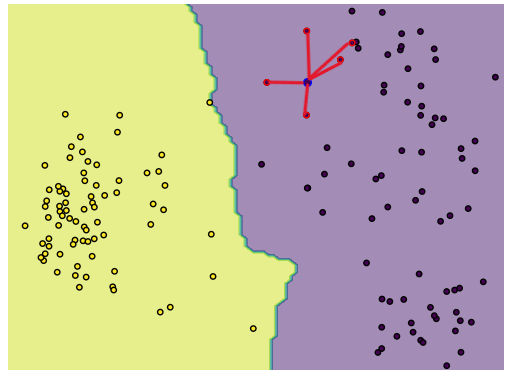
\includegraphics[width=0.5\linewidth]{graphics/knn_classification.png}
    \caption{A KNN-classifier has been trained on the displayed training data. The blue example will be classified as purple, because its nearest neighbors are purple. The decision boundary is very complicated -- this is usual for KNN-classifiers.}
\end{figure}

\begin{figure}
    \centering
    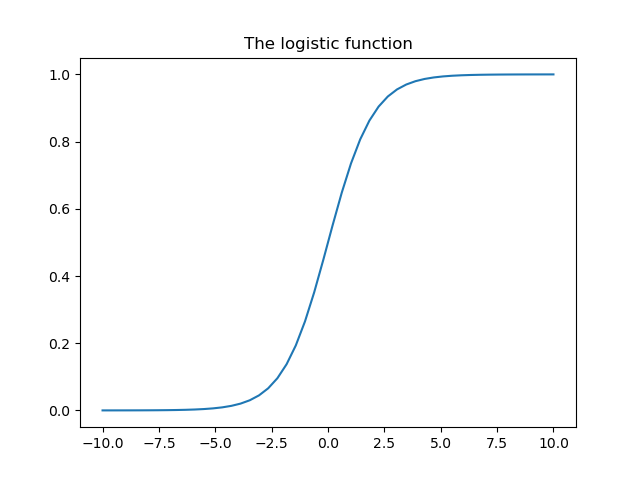
\includegraphics[width=0.5\linewidth]{graphics/logistic.png}
    \caption{The logistic function}
\end{figure}

\subsection{Logistic regression} Let us consider the two-class case. We want to design a model that gives us an estimate of the \emph{probability} that $y$ is equal to $1$ \emph{conditioned} on $x$:
\begin{align*}
    p(x) = \mathbb{P}(y=1 \, \vert \, x).
\end{align*}
\emph{Logistic regression} is conceptually very simple to explain -- simply take a linear predictor $\sprod{\beta,x}$ and insert into  model the \emph{logistic function} $\varphi(x)=e^x/(1+e^x)$
\begin{align*}
    p_\beta(x) = \frac{e^{\sprod{\beta,x}}}{1+e^{\sprod{\beta,x}}}
\end{align*}
for some $\beta$. There are different ways to motivate this. The simples one is to simply look at the logistic function -- it is a smooth, $s$-shaped curve that goes to $0$ when the argument is small and goes to $1$ when the argument is  large. Hence, the 'largeness' of $\sprod{\beta,x}$ becomes an indicator of the probability, and the probability gets less extreme as we move away from the non-extreme values of it.

A bit more transparent way of motivating it is given by the concept of \emph{odds}. The odds $o$ of an event is defined as the probability that it happens divided with the probability that it does not happen, i.e.
\begin{align*}
    o = \frac{p}{1-p}.
\end{align*}
So if the odds are $2$ ('$2$ to $1$'), it is twice as likely that an event happen than it is to not happen -- that is, $p=\tfrac{2}{3}$. It is simple to see that 
\begin{align*}
    p = \frac{o}{1+o}.
\end{align*}
That means that in logistic regression, we assume that the \emph{logarithm of the odds} (or simply log-odds) of $y=1$ is given by a linear function $\sprod{\beta,x}$. If we increase the value of $\sprod{\beta,x}$ by $1$, the odds increases by a factor of $e$.

\paragraph{Remark:} A source of confusion is that the 'odds' as we define it here is \emph{not} what a bookmaker would list as 'odds'. What is listed on most bookmaker sites is rather the \emph{payout} $R$ on a bet of the size $1$. That is, if the event you are betting on happens, the net win for you is $R-1$, and if not, the net 'win' is $-1$. This is fair if it is $(R-1)$ times as likely that the event \emph{does not} happen than that it does. Hence, the payout and odds are related as $o=1/(R-1)$ (which leads to the simple relation $p=1/R$ between the payout and the probability, assuming fair odds).


\subsubsection{Fitting a logistic regressor: The principle of \emph{maximum likelihood}}
We find the optimal $\beta$ via fitting it to our data. We could make a least squares fit -- i.e. try to minimize
\begin{align*}
    \sum_{k\in [n]} \norm{y_k - p_\beta(x_k)}^2.
\end{align*}
It is much more elegant, to instead \textbf{maximize the likelihood} of the data. That is, for each value of $\beta$, we check the probability of the observed labels $y_k$ given the observed data $x_k$. Since the observations are assumed to be independent, that probability is equal to
\begin{align*}
    \max_\beta \ell(\beta) =  \max_\beta \Pi_{k \in [n]} \mathbb{P}(y \,\vert \, x_k) = \Pi_{y_k =1} p(x_k)\cdot \Pi_{y_k=0} (1-p(x_k)).
\end{align*}
The above function is the likelihood. We now choose the value of $\beta$ that makes the likelihood as big as possible. 

Maximizing the likelihood is of course equivalent of maximizing the logarithm of the likelihood, which is equivalent to minimizing the negative logarithm of the likelihood. One therefore often also formulate the problem as \emph{minimizing the negative log-likelihood}. This turns the product (which is there due to the independence of the $x_k$) into a sum:
\begin{align*}
    \min_{\beta} - \log(\ell(\beta)) &= \min_\beta \sum_{y_k=1} -\log(p(x_k)) + \sum_{y_k=0} -\log((1-p_k)) \\
    &= \min_\beta \sum_{k \in [n]} -y_k\log(p_k)-(1-y_k)\log(1-p_k) 
\end{align*}
This loss function is sometimes referred to as the \emph{cross entropy loss} (for reasons we will not go into here).

To actually classify examples, we output a $1$ if the probability $p_1(x)$ is bigger than some threshold $\theta_*$. ($\theta_*=.5$ is a rational choice, but other thresholds might lead to better performance). Since $p_1(x)$ is a function of $\sprod{\beta,x}$, the decision boundary will be a plane of the form $\sprod{\beta,x}=v(\theta^*)$. One speaks of a linear decision boundary.

\subsubsection{Multiple classes} We can use logistic regression to build a model for the case of $y$ taking on more than one value -- that is, the case of $K$ classes. Let us say that $y$ can take on the values $0,\dots, K-1$. The assumption here is to assume that the relative log-odds
(that is, $\log(\mathbb{P}(y=k \, \vert \, x)/\mathbb{P}(y=\ell \, \vert \, x ))$) between any two classes is linear in $x$. This is accomplished by the following model:
\begin{align*}
    p_{k,\beta}(x) = \mathbb{P}(y=k \, \vert \, x) = \frac{e^{\sprod{\beta_k,x}}}{\sum_{\ell\in [K]}e^{\sprod{\beta_\ell,x}}}.
\end{align*}
Note that we here divide the value of $e^{\beta_k,x}$ with the sum of all $e^{\sprod{\beta_\ell,x}}$. This means that the sum of all $p_{k,\beta}(x)$ is equal to $1$, and we can interpret $(p_{k,\beta}(x))_{k\in[K]}$ as a probability distribution.

One speaks of the \emph{softmax}-coding -- the vector ($\sprod{\beta_k,x})_{k\in [K]}$ (which is linear in $x$ is put through the \emph{softmax} function
\begin{align*}
    \mathrm{softmax}(y)_i = \frac{e^{y_i}}{\sum_{k \in [K]}e^{y_k}}.
\end{align*}
Note that this is a 'soft' approximation of the 'amax' function
\begin{align*}
    \mathrm{amax}(y)_i = \begin{cases}
        1/m \text{ if } y_i \text{ is the largest entry in $y$, and there are $m$ such maximizers } \\
        0 \text{ else.}
    \end{cases}
\end{align*}
We still determine the best $\beta$ via maximizing the likelihood:
\begin{align*}
    \max_\beta \Pi_{k \in [K]} \Pi_{y_i=k} p_{k,\beta}(x_i)
\end{align*}
or also minimizing the negative log-likelihood:
\begin{align*}
    \min_\beta \sum_{k \in [K]} \sum_{y_i=k} - \log(p_{k,\beta}(x_i)).
\end{align*}
It is not hard to see that an example is assigned to the $k$ for which $\sprod{\beta_k,x}$ is largest. The \emph{decision boundaries}, i.e. sets where more than one class is equally likely, are thus linear subspaces $\sprod{\beta_k,x}=\sprod{\beta_\ell,x}$.

\subsection{Outlook: Generalized Linear Models}
Logistic regression, as is standard linear regression, is a special case of a so-called \emph{generalized linear models}. The basic assumption of a generalized linear model is that given the value of $x$, the label $y$ follows a one-parameter distribution where the parameter depends on a linear feature $\sprod{\beta,x}$ in  a certain way. This distribution is then fitted to the data at hand, for instance through maximum likelihood.

The family of distribution is most often assumed to be a so-called \emph{exponential family}. For a continuous variable, that is a family of variables with probability distribution functions of the form\footnote{One can also allow a probability measure of the form $h(y) \exp(\sprod{\theta,T(y)} - A(\theta)) $ f or a function $T$ -- one then simply needs to transform the data $z_i=T(y_i)$ to return to the formulation discussed here}
\begin{align*}
    p(y \, \vert \theta ) = h(y) \exp(\sprod{\theta,y} - A(\theta))
\end{align*}
and in the discrete case, a probability mass function of the form
\begin{align} 
    \mathbb{P}(y=k \, \vert \theta) =  h(k) \exp(\sprod{k,\theta} - A(\theta))
\end{align}
$\theta$ is parametrizing the family. In a generalized linear model, we assume that this entity is a linear function of the features: If $y$ is scalar, this boils down to $\theta=\sprod{\beta, x}$, where $\beta$ is to be estimated. The determination of the maximum likelihood estimate (negative log likelihood-minimization) turns into the problem
\begin{align} \label{eq:maxlikelihood}
    \min_\beta \sum_k A(\sprod{\beta,x_i})-y_i\sprod{\beta,x_i} - \log(h(y_i)).
\end{align}
If we assume that $A$ is convex, this is a convex minimization problem, that hence can be solved with standard methods.

It is more common to express the generalized linear model through a so called \emph{link function}. One can show (see the exercises) the following relation for the expected value:
\begin{align}
     \erw(z \, \vert \theta) = A'(\theta). \label{eq:mean}
\end{align}
Since we have assumed that $A$ is convex, $A'$ will be injective, so that it can be inverted. This means that the model assumption can be in an inverse form, which often is done:
\begin{align*}
    g(\mu) = g( \erw(z \, \vert \theta)) = \sprod{\beta,x}.
\end{align*}
The function $g$ is the so-called \emph{link function}, the inverse of $A'$.

To make this a bit more clear, let us consider three examples:

\paragraph{Linear regression} Assuming that $y$ conditioned on $\theta$ is a Gaussian (with a fixed variance $\sigma$) is contained in the above framework:
\begin{align*}
    p(y \, \vert \, \theta) = \frac{1}{\sqrt{2\pi\sigma^2}} \exp\left(-\frac{(y-\mu)^2}{2\sigma^2}\right) = \frac{e^{-\tfrac{y^2}{2\sigma^2}}}{\sqrt{2\pi\sigma^2}}\exp (\theta y - \tfrac{\sigma^2}{2}\theta^2) \\ \quad \theta = \frac{\mu}{\sigma^2}
\end{align*}
Here, the link function is $g(\mu) =\frac{\mu}{\sigma^2}$. Modelling $\theta = \sprod{\beta,x}$, we quickly obtain that the negative log-likelihood is seen to be equal to (up to a constant)
\begin{align*}
    \tfrac{1}{2\sigma^2} \sum_{k}(y_k-\sprod{\beta,x_k})^2
\end{align*}
Least square-fitting is hence the same as fitting a random variable with a mean linearly dependent of the feature and a constant variance!

\paragraph{Logistic regression} Our Bernoulli-variable from above has the form
\begin{align*}
      \mathbb{P}(z=k \, \vert \theta) = \begin{cases} \frac{o^k}{1+o} & \text{ k = 0,1 } \\ 0 & \text{ else} \end{cases}
\end{align*}
where $o$ is the odds (insert $k=0$ and $k=1$ to see that it is true!). This can also be written as follows:
\begin{align*}
    \frac{o^k}{1+o} = \exp(k\log(o)-\log(1+o)) = \exp(k\theta - \log(1+e^\theta)), \quad \theta =\log(o), A(\theta) = \log(1+e^\theta)
\end{align*}
We see what we saw before: $\theta$, the object modelled as a linear function of the features, is the log-odds. The link function is $g(\mu) = \log(\mu/(1-\mu))$.

\paragraph{Poisson regression} A \emph{Poisson-variable} with \emph{rate} $\lambda>0$ is an $\N$-valued variable with the probability mass function
\begin{align*}
    \mathbb{P}(y=k) = \frac{\lambda^ke^{-\lambda}}{k!}.
\end{align*}
It is often used to model a random number of occurances of an event in a fixed time, such as the number of earthquakes in a year, days in a month with very hot temperatures, or number of goals in a football match. (If one assumes that the time between occurances are independent from each other and exponentially distributed, the number of occurances within a fixed time frame will be Poisson distributed).

Poisson-variables can be put into the exponential family framework:
\begin{align*}
   \frac{\lambda^ke^{-\lambda}}{k!} =  \frac{1}{k!}\exp(k\log(\lambda)-\lambda) = \frac{1}{k!}\exp(k\theta - e^\theta), \quad  \theta = \log(\lambda), A(\theta) = e^\theta. 
\end{align*}
The link function is $g(\mu)=\frac{1}{\mu}$. Poisson regression corresponds to assuming that the logarithm of the rate is linear in the features.

\paragraph{Some more prominent examples} The generalized linear model framework is more flexible than this -- the nature of the data determines which exponential family is best suited. A few examples include exponential (modeling wait times), binomial (modelling number of successes in a fixed number of trials), negative binomial (modelling times until failure) and log-normal (modelling objects which grow randomly but always proportionally to size, e.g. stock prices).


\subsection{Discriminant analysis} 
Let us finally consider a completely different approach than logistic regression: \emph{discriminant analysis}. The approach is in some sense the complete inverse of what we did above: Instead assuming a form of the distribution of the label $y$ conditioned on the values of the features $x$, we assume that the \emph{features $x$} have a distribution of a certain form \emph{dependent on the labels $y$}. That is, \emph{within each class},
the data points $x_k$ are distributed according to some probability distribution dependent on the class $k$:
\begin{align*}
    \mathbb{P}(x \, \vert y=k)= p_k(x). 
\end{align*}
Choosing a particular model for $p_k$ amounts making a \emph{prior} assumption on the $x$.

Fitting this prior is in of itself not that interesting however -- we are ultimately interested in $\mathbb{P}(y=k \, \vert x)$. We can however calculate this probability with the help of Bayes' theorem:
\begin{align*}
    \mathbb{P}(y=k \, \vert \, x) = \mathbb{P}(x \, \vert y=k) \cdot \frac{\mathbb{P}(y=k)}{\sum_{\ell\in [K]}\mathbb{P}(x \, \vert \, y=\ell) \mathbb{P}(y=\ell)}
\end{align*}
Let's simplify that notation -- with $\pi_\ell= \mathbb{P}(y=\ell)$ and $p_k(x) = \mathbb{P}(x \, \vert \, y=k)$, we get
\begin{align*}
    \mathbb{P}(y=k \, \vert \, x) = \frac{p_k(x) \pi_k}{\sum_\ell p_\ell(x)\pi_\ell}.
\end{align*}
To classify an example, we simply calculate the above quantities and return the largest one (or equivalently the one whose log is the largest). We hence need to maximize
\begin{align*}
    \log(p_k(x)) + \log(\pi_k) - \log\left( \sum_{\ell}\pi_\ell(x) \pi_\ell\right).
\end{align*}
Note that $\log\left( \sum_{\ell}\pi_\ell(x) \pi_\ell\right),$ is common for all terms, so that we are actually only maximizing $\delta_k(x)=\log(p_k(x))+\log(\pi_k)$. These are called \emph{discriminants}. The probabilities $\pi_k$ can easily be estimated as simply the fraction of datapoints belonging to the class $k$. To estimate $\log(p_k(x))$ is harder, but for reasonable prior assumptions possible. 

\paragraph{Remark} We call these models \emph{generative} since we, in principle, after fitting the $p_k$ could 'generate' $x$'s from class $k$ via sampling them from $p_k(x)$. 



\subsubsection{Linear discriminant analysis}  The probably simplest model assumption is that the $x$ within each class are Gaussian distributed, i.e.
\begin{align*}
    p_k(x) = \det(2\pi\Sigma)^{-1/2} \exp( -\tfrac{1}{2}\sprod{x-\mu_k,\Sigma^{-1}(x-\mu_k)}),
\end{align*}
where $\Sigma$ is a covariance matrix and $\mu_k$ are means. Note that we have assumed that the $\Sigma$ is common for all classes, while the $\mu_k$ are unique to each class -- this is the assumption leading to \emph{linear discriminant classifiers}.

What is $\log(p_k(x))$ for this model? We have
\begin{align*}
    \log(p_k(x)) &= - \tfrac{1}{2}\sprod{x-\mu_k,\Sigma^{-1}(x-\mu_k)} - \tfrac{1}{2}\log \det(\Sigma) \\
        &= \sprod{x,\Sigma^{-1}\mu_k} -\tfrac{1}{2}\sprod{\mu_k,\Sigma^{-1}\mu_k}-\underbrace{\sprod{x,\Sigma^{-1}x}- \tfrac{1}{2}\log(\det(2\pi\Sigma))}_{\text{independent of $k$}}.
\end{align*}
We can hence use
\begin{align*}
    \delta_k(x) = \sprod{x,\Sigma^{-1}\mu_k} -\tfrac{1}{2}\sprod{\mu_k,\Sigma^{-1}\mu_k} + \log(\pi_k).
\end{align*}
as discriminants. These are linear, hence the name linear discriminant analysis. We now only need to plug estimates for $\mu_k$, $\Sigma$ and $\pi_k$ in the discriminants to obtain a model. These are obvious choices (with $n_k$ equal to the the number of $y_i$ in class $k$):
\begin{align*}
    \hat{\mu}_k &= \frac{1}{n_k} \sum_{i: y_i =k} x_i \\
    \widehat{\Sigma} &= \frac{1}{N-K}\sum_{k\in [K]} \sum_{i : y_i =k}(x_i-\hat{\mu}_k)(x-\hat{\mu}_k)^* \\
    \hat{\pi}_k &= \frac{n_k}{n}
\end{align*}
(The factor $\tfrac{1}{N-K}$ in the estimate for $\Sigma$ ensures that the estimate is unbiased).

\subsubsection{Quadratic discriminant analysis} What happens when we drop the assumption that the covariance matrix $\Sigma$ is equal for all classes? That is, we assume 
\begin{align*}
    p_k(x) = \det(2\pi\Sigma_k)^{-1/2} \exp( -\tfrac{1}{2}\sprod{x-\mu_k,\Sigma_k^{-1}(x-\mu_k)}).
\end{align*}
Then, $\log(p_k(x))$ takes on the form
\begin{align*}
    \log(p_k(x)) =  \sprod{x,\Sigma_k^{-1}\mu_k} -\tfrac{1}{2}\sprod{\mu_k,\Sigma_k^{-1}\mu_k}-\sprod{x,\Sigma_k^{-1}x}- \tfrac{1}{2}\log(\det(2\pi\Sigma_k)).
\end{align*}
Note that none of the terms here are independent of $k$. Hence, the discriminants will be \emph{quadratic} in $x$:
\begin{align*}
     \delta_k(x) = \sprod{x,\Sigma_k^{-1}\mu_k} -\tfrac{1}{2}\sprod{\mu_k,\Sigma_k^{-1}\mu_k}-\sprod{x,\Sigma_k^{-1}x}- \tfrac{1}{2}\log(\det(2\pi\Sigma_k)) +\log(\pi_k).
\end{align*}
The only thing we need to change compared to the linear discriminant analysis is the estimates for the covariance matrices, e.g.
\begin{align*}
     \widehat{\Sigma}_k &= \frac{1}{n_k-1}\sum_{k\in [K]} \sum_{i : y_i =k}(x_i-\hat{\mu}_k)(x-\hat{\mu}_k)^*.
\end{align*}
QDA is more flexible than LDA -- in particular, its decision boundaries are quadratic surfaces, and not only linear. It may for certain classification problems thus have lower bias -- this depends on the geometry of the true decision boundaries. However, it will have higher variance, since we need to estimate one covariance matrix per class. This is especially problematic if some classes have very few observations.


\subsection{Evaluation of classifiers}
In general, classifiers are evaluated as any other model, i.e. through performance on a test set. This may be too blunt though -- imagine a very unbalanced data set of two classes, say with $\mathbb{P}(y=1)=98\%$. Then the classifier that assigns $1$ to all example has an error rate of only $2\%$! It will then however misclassify all $x$ belonging to the class $0$. Let us here give two ways to more quantitatively evaluate a classifier.

\paragraph{Confusion matrices } A more comprehensive way to evaluate the performance of a classifier is a \emph{confusion matrix}. The entry $c_{ij}$ of a confusion matrix is the fraction of $x$ in class $i$ that is assigned class $j$ by the classifier. Optimally, a confusion matrix should have ones on the originals and zeros rest. Using the confusion matrix, we can see whether certain classes are more often misclassified. For an example, see Figure \ref{fig:error_metrix}.

\begin{figure}
    \centering
    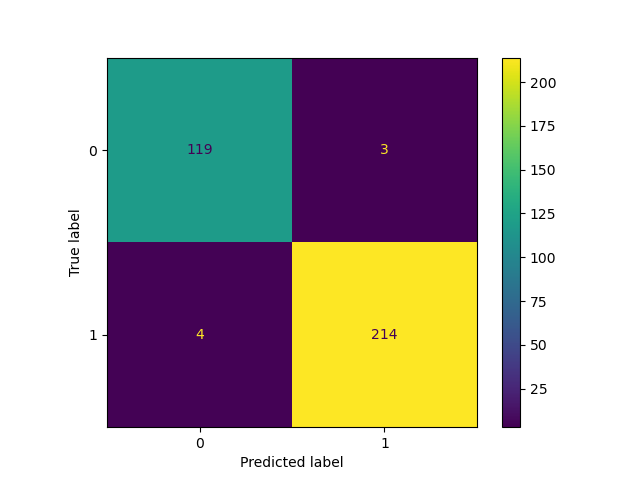
\includegraphics[width=0.31\linewidth]{graphics/confusion_matrix.png}
    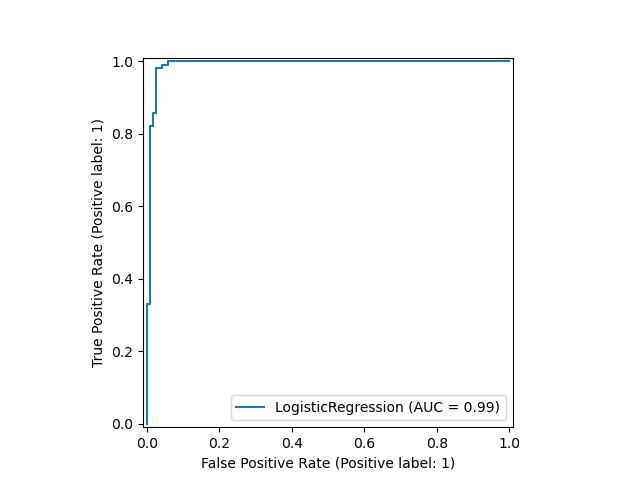
\includegraphics[width=0.31\linewidth]{graphics/pr.png}
    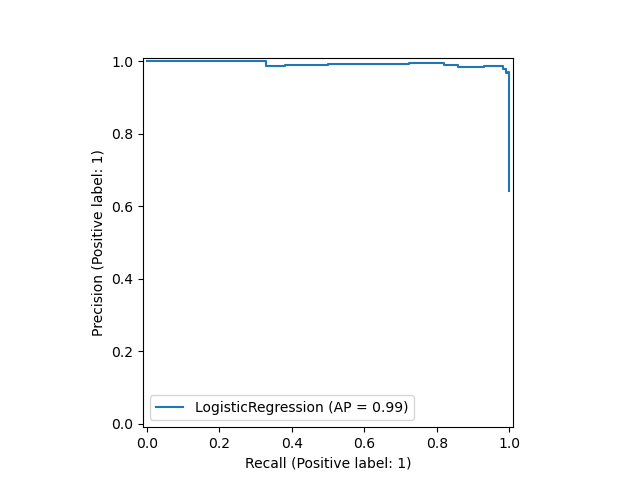
\includegraphics[width=0.31\linewidth]{graphics/roc.png}
    \caption{A confusion matrix, a precision-recall-curve and ROC-curve for a logistic classifier trained on a split of the '\texttt{breast\_cancer}'-dataset from \texttt{sklearn} package. Shown are results on the test set.}
    \label{fig:error_metrix}
\end{figure}

\paragraph{ROC-curves} Another way to visualise the performance of a classifier with two classes is a so-called $ROC$-curve. Remember that $p_{\beta}(x)$ is our estimated probability that an example belongs to class $1$. Although this means that it is reasonable to assign an example to class $1$ as soon as $p_\beta>.5$, we can actually choose to do it when $p_\beta \geq p_*$ for any $p_*$ we choose. Choosing $p_*$ low will probably mis-classify more $0$:s as $1$ and vice-versa. For each $p_*$, we will get a \emph{true positive rate} and a \emph{false positive rate}
\begin{align*}
    \text{ True positive rate}&= \frac{\text{Number of examples correctly classified as $1$}}{\text{Number of examples in class $1$ }} \\
    \text{False negative rate}&= \frac{\text{Number of examples incorrectly classified as $1$}}{\text{Number of examples in class $1$ }}
\end{align*}
The curve of traced out by changing the value of $p_*$ in a true-positive/false negative space is known as the $ROC$ curve (see Figure \ref{fig:error_metrix}) The optimal $ROC$-curve is the one with true positive rate $1$ for all false negative rates. Hence, the higher the area under the curve, the better, and therefore, this area (AUC) is sometimes used as a quantative measure of quality of the estimator.

Other measures to describe the quality of a classifier are 
\emph{precision} and a \emph{recall}
\begin{align*}
    \text{Precision}&= \frac{\text{Number of examples correctly classified as $1$}}{\text{Number of examples classified as $1$ }} \\
    \text{Recall}&= \frac{\text{Number of examples correctly classified as $1$}}{\text{Number of examples in the class $1$ }}
\end{align*}
Making a similar plot as above produces a precision-recall curve. See Figure \ref{fig:error_metrix}.



\subsection{Further reading}
Classification with logistic regression, LDA and QDA are discussed in Chapter 4.1,4.2,4.3 and 4.4 of 'Introduction to Statistical Learning. Recommended exercises in the same book to have a look at are 4.5, 4.6,4.7, 4.8,4.10, 4.12 . Exercise 4.4 is a bit more challenging, but a really good food for thought to understand the problems of high dimensions in general.

 Consider also the following exercises.

\begin{exercise}
    Show that solving \eqref{eq:maxlikelihood} exactly corresponds to determining the maximum likelihood estimate of $\beta$.
\end{exercise}

\begin{exercise}
    Derive the forms of the link functions for Bernoulli and Poission variables (you only need to invert the formula  $\mu = A'(\theta)$ to get to $g(\mu)=\theta$.)
\end{exercise}

\begin{exercise}
    The purpose of this exercise is to derive the formula \ref{eq:mean}. We will for simplicity do the derivation for the discrete case for scalar $k$, but the argument is exactly the same as for the continuous case and multidimensional case

    \begin{enumerate}[(a)]
        \item Argue that
        \begin{align*}
            \sum_{k=0}^\infty h(k) \exp(k\theta-A(\theta)) =1
        \end{align*}
        for all values of $\theta$.
        \item By taking the derivative of the above equation, show that
        \begin{align} \label{eq:formulaone}
            \sum_{k=0}^\infty h(k)(k-A'(\theta))\exp(k\theta-A(\theta)).
        \end{align}
       (Note that the series we are working with essentially is a power series, so differentiation can be performed term-wise).
        \item Argue that \eqref{eq:formulaone} implies \eqref{eq:mean}.
    \end{enumerate}
\end{exercise}

\begin{exercise} This is a challenging, but rewarding exercise. It relates to so-called \emph{naive Bayes estimators}, that we have skipped in the lecture -- but it can be solved without knowledge about what they are.

    Consider a dataset of binary quadratic images, i.e. matrices of size $N\times N$ filled with either zeros or ones, divided into $K$ classes. We now define a generative model for class $k$ via letting the value of each pixel $(i,j)$ be one with a probability $p_{ij}^k$, and zero else (i.e., the pixels are independent Bernoulli variables).
    \begin{enumerate}[(a)]
        \item Derive a formula for $p_k(x)$, in dependence of the parameters $p_{ij}^k$. \emph{Hint: What are the possible values for $x$ in this example?}
        \item Show that the average log-likelihood of a sample is maximized when the parameters $p_{ij}^k$ are chosen as
        \begin{align*}
            p_{ij}^k = \mathbb{P}(\text{ Pixel $(i,j)$ is one} \, \vert \, x \text{ is in class } k).
        \end{align*}
        \item Generate a dataset of binary images from the \texttt{digits} data-set in \texttt{sklearn} and estimate the $p_{ij}^k$. Sample images from the resulting distributions for each $k$. Comment on the appearance of the samples. (This should make the meaning of  \emph{generative} models more clear!)
        \item Redo (c), but now only use a subset of the images to estimate the $p_{ij}^k$. What test performance do you get?
    \end{enumerate}
\end{exercise}




\section{Support vector machines}
Let us take a step back, and have a look at logistic regression and linear discriminant analysis in the case of two classes. When all is said and done, what we are doing for both these models is to decide on a linear subspace that serves as our decision boundary. Here, we choose the 
'best' subspace indirectly - we try to fit distributions to our data. Why don't we instead use a more direct, geometrical criterion to choose it?


Deciding on a linear classifier is the same thing as determining a hyperplane $\gamma + \sprod{\alpha,x}$  To simplify the notation, let us as usual attach a $1$ to each $x$, $x\to [1,x]$ and write $\gamma + \sprod{\alpha,x} = \sprod{[\gamma,\alpha},[1,x]=\sprod{\beta,x}$. In order for the hyperplane to be a  decision boundary consistent with the training data, we need all datapoints in one class is one one side of it, i.e. $\sprod{\beta,x}<0$ and the other ones on the other side, $\sprod{\beta,x_i}>0$. If we call the classes $y=1$ and $y=-1$, and let $y=1$ correspond to the side of the hyperplane $\sprod{\beta,x}>0$, a hyperplane is then consistent with the training data if and only if
\begin{align*}
    y_i \sprod{\beta,x_i}>0, \quad i \in [n].
\end{align*}
We call all planes satisfying the above \emph{separating hyperplanes}. Now, if there is such a hyperplane, there will very probably be infinitely many. Which one of them should we choose?

Optimally, we should strive for the (training) data points to be as far away from the decision boundary as possible. In that way, the classification procedure should intuitively become more stable. We would hence like to solve the following optimization problem
\begin{align*}
    \max_\beta \min_{i \in [n]} \dist(x_i,H_\beta) \text{ s.t. } y_i \sprod{\beta,x_i}>0, i \in [n].
\end{align*}
where $H_\beta$ is the hyperplane $\{x \, \vert \sprod{\beta,x}=0\}$. $ \min_{i \in [n]} \dist(x_i,H_\beta)$ is called the \emph{margin} of the separating hyperplane. It is a a standard result of linear algebra  that
\begin{align*}
    \dist(x,H_\beta) = \frac{\abs{\sprod{\beta,x}}}{\norm{\beta}_2}.
\end{align*}
Note that provided $y_i \in \{-1,1\}$ and $y_i\sprod{\beta,x_i}>0$, $y_i\sprod{\beta,x_i} = \abs{\sprod{\beta,x_i}}$. Hence, our problem turns into
\begin{align*}
    \max_\beta \min_{i \in [n]}\frac{y_i\sprod{\beta,x}}{\norm{\beta}_2}\text{ s.t. } y_i \sprod{\beta,x_i}>0, i \in [n].
\end{align*}
This problem is scale-invariant in $\beta$ -- multiplying $\beta$ with a positive scalar does not change the value of the function that we are optimizing. We hence need to normalize it to make it have a unique solution. We could only consider $\beta$ with $\norm{\beta}_2=1$, but it is actually more clever to only consider $\beta$ with $\min_{i \in [n]} y_i \sprod{\beta,x_i}\geq 1$. Then, the problem gets the form
\begin{align}
    & \max_\beta \frac{1}{\norm{\beta}_2}\text{ s.t. } y_i\sprod{\beta,x_i}>1, i \in [n] \nonumber \\
     =& \min_\beta \tfrac{1}{2}\norm{\beta}_2^2 \text{ s.t } y_i\sprod{\beta,x_i}\geq 1, i \in [n] \label{eq:SVM}
\end{align}
The last problem is the standard form of the \emph{maximal margin linear support vector machine} (or maximal margine linear SVM, or maximal margin support vector classifier). This form is slightly different compared to the one in \cite{james2023introduction} -- the reason we consider this form is that it is easier to analyse mathematically.

\subsection{Soft margins} For most data sets, there are no separating hyperplanes -- due to errors, the classes will 'bleed' across the even the best linear decision boundary. How do we handle that case? We need to allow some training examples to be misclassified. We can do this by relaxing our hard constraint $y_i \sprod{\beta,x_i}\geq 1$ to be violated slightly -- that is, $y_i\sprod{\beta,x_i}\geq 1 -\epsilon_i$ for some \emph{slack variables} $\epsilon_i\geq 0$. We do not want those violations to be too common or too severe, and should hence penalize them. This leads to the \emph{soft margin} SVM problem:
\begin{align}
    \min_\beta \tfrac{1}{2}\norm{\beta}_2^2 + \lambda \sum_{i\in [n]} \epsilon_i \text{ s.t } y_i\sprod{\beta,x_i}\geq 1-\epsilon_i, i \in [n] , \epsilon_i \geq 0\label{eq:SVMsoft}
\end{align}
This is the default problem that is solved by \texttt{sklearn}! The \texttt{C}-parameter in \texttt{sklearn} corresponds to the $\lambda$ above. 

\subsection{More than two classes} There are two ways to use SVM:s to classify objects in more classes. Either, we train one SVM per class, to decide whether the object belongs to the class or not (\emph{'one versus all'} or \emph{'one-vs-rest'}, and then assign the example to the $k$ so that $\sprod{\beta_k,x}$ is the largest, since this corresponds to 'high confidence' 

The other strategy is to train a binary classifier for each pair of classes (\emph{'one vs one'}). We then assign an example via counting how many 'votes' each class gets in the pair-wise comparison, and choose the class with the most votes. Using a one-vs-one strategy is sometimes more expensive, but not always -- we will need to fit $\sim K^2$ models instead of $\sim K$, but each fit will on the other hand work with less data. Which strategy to prefer is hence situation dependent.

\subsection{Support vectors}
Why are these classifiers called \emph{support vector machines}? At the optimum $\beta^*$ of \eqref{eq:SVM}, there must be a number of data vectors $x_i, i\in I$ which are on the decision boundary, i.e  $y_i\sprod{\beta_*,x_i}=1$. These vectors are called the \emph{support vectors}. See also Figure \ref{fig:svm}. These completely decide the decision boundary in the sense that if we, after obtaining a $\beta_*$, change the data-points $x_i$ with $y_i \sprod{\beta_*,x_i}>1$ in a way so that they still obey $y_i \sprod{\beta_*,x_i}>1$, $\beta_*$ will remain the solution of the problem. In this way, the SVM estimate is stable towards outliers far away from the decision boundary.

\begin{figure}
    \centering
    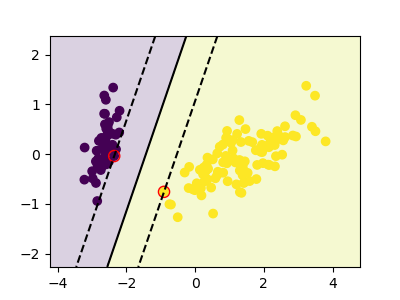
\includegraphics[width=0.5\linewidth]{graphics/svm_classifier.png}
    \caption{An svm classifier has been trained to detect one of the classes in the \texttt{iris} dataset (purple). We have trained it on the top-2-scores resulting from a PCA, to be able to easily visualize it. Shown is the optimal separating hyperplanes, as well as the support vectors (marked with red boundaries), and the lines $\sprod{\beta^*,x_i}=\pm 1$. Best viewed in color. }
    \label{fig:svm}
\end{figure}

How can we formally prove this property of the SVM? For that, we need to take a small detour into the theory of convex optimization. It will seem like a unnecessary long detour right now, but it will help us also in the following. 

Let us define the  \emph{Lagrangian} function for the problem \eqref{eq:SVM}
\begin{align*}
    L(\beta, \gamma) = \tfrac{1}{2}\norm{\beta}_2^2 + \sum_{i\in [n]}(1-y_i\sprod{\beta,x_i})\gamma_i, \quad \beta \in \R^p, \R^n \ni \gamma \geq 0.
\end{align*}
If we have $y_i\sprod{\beta,x_i}\geq 1$ for all $i$, we actually have $\sup_{\gamma \in \R^n} \sum_{i\in [n]}(1-y_i\sprod{\beta,x_i})\gamma_i =0$, and otherwize, the supremum is $+\infty$. Hence, what we are solving in \eqref{eq:SVM} is actually
\begin{align*}
    \min_{\beta}\sup_{\gamma\geq 0} L(\beta,\gamma).
\end{align*}
Now, can we interchange the minimum and the supremum? Not in general. However, we have the following.
\begin{theorem}
    Consider an optimization problem of the form
    \begin{align*}
        \min_{\beta} f(\beta) \text{ s.t. } g_i(\beta) \leq 0, i\in [K]
    \end{align*}
    for convex functions $f$ and $g_i$, and the corresponding Lagrangian
    \begin{align*}
        L(\beta,\gamma) = f(\beta) + \sum_{i \in [K]}\gamma_i g_i(\beta), \quad  \gamma \geq 0.
    \end{align*}
    \begin{enumerate}
        \item \emph{Weak duality} always holds
        \begin{align*}
            \min_\beta \sup_{\gamma \geq 0} L(\beta,\gamma) \geq \sup_{\gamma\geq 0 }\min_{\beta} L(\beta,\gamma).
        \end{align*}
        \item If either all $g_i$ are affine-linear and there exists a $\beta$ with $g_i(\beta)\leq 0$ for all $i$, \emph{or} there exists a $\beta$ with $g_i(\beta)<0$ for all $i$, \emph{strong duality} holds
        \begin{align*}
            \min_\beta \sup_{\gamma \geq 0} L(\beta,\gamma) = \sup_{\gamma\geq 0}\min_{\beta} L(\beta,\gamma).
        \end{align*}
    \end{enumerate}
\end{theorem}
This theorem is really tricky to prove, and relies on theory of convex geometry\footnote{Interested readers are directed to the excellent \cite{boyd2004convex}}. Let us skip it and instead introduce a bit more jargon. The  problem
\begin{align*}
    \sup_{\gamma\geq 0 }\min_{\beta} L(\beta,\gamma)
\end{align*}
is an optimization problem in $\gamma$. This problem is referred to as the \emph{dual problem} (and the original one as the \emph{primal problem}). What is the dual problem of the SVM problem?
\begin{prop}
    The dual problem of \eqref{eq:SVM} is
    \begin{align*}
        \sup_{\gamma \geq 0 } \sum_{i \in [n]} \gamma_i - \tfrac{1}{2} \norm{\sum_{i \in [n]}\gamma_i y_i x_i}_2^2.
    \end{align*}
    Strong duality holds if there exists a $\beta_0$ with $y_i\sprod{\beta,x_i} \geq 1$ for all $i$.
\end{prop}
\begin{proof}
First, strong duality follows from the fact that the constraint functions $g_i(\beta)=(1-y_i\sprod{\beta,x_i})$ are all affine-linear. Now, we need to calculate
    \begin{align*}
        \min_\beta \tfrac{1}{2}\norm{\beta}_2^2 +  \sum_{i \in [n]} \gamma_i(1-y_i\sprod{\beta,x_i}) = \min_{\beta} \sum_{i \in [n]} \gamma_i + \tfrac{1}{2}\norm{\beta}_2^2 - \sprod{\beta, \sum_{i\in [n]}\gamma_i y_i x_i}
    \end{align*}
    This is however a simple quadratic problem -- the optimum is characterized by
    \begin{align*}
        \beta - \sum_{i\in [n]} \gamma_i y_i x_i =0,
    \end{align*}
    so that
    \begin{align*}
        \min_\beta \tfrac{1}{2}\norm{\beta}_2^2 + \sum_{i \in [n]} \gamma_i(1-y_i\sprod{\beta,x_i}) =  \sum_{i \in [n]} \gamma_i - \tfrac{1}{2} \norm{\sum_{i \in [n]}\gamma_i y_i x_i}_2^2,
    \end{align*}
    which was the claim.
\end{proof}

We know that in the case of strong duality, the optimal values of the primal and dual problems coincide. There is also a relation between the solution of the problems.
\begin{theorem}
    Suppose that strong duality holds. Then, following are equivalent for a pair $(\beta^*,\gamma^*)$.
    \begin{enumerate}[(i)]
        \item $\beta^*$ is a solution to the primal problem and $\gamma^*$ is a solution to the dual problem.
        \item $L(\beta^*,\gamma^*) = \inf_{\beta} L(\beta,\gamma^*) = \sup_\gamma L(\beta^*,\gamma)$, and 
            \begin{align}
    \sum_{i \in [K]} \gamma_i^* g_i(\beta^*)=0 \label{eq:slackness}.
    \end{align}
    \end{enumerate}
\end{theorem}
\paragraph{Remark} \eqref{eq:slackness} is called the \emph{complimentary slackness condition}.

\begin{proof}
    (i)$\Rightarrow$ (ii). By the fact that the primal optimal solution obeys $g_i(\beta^*)\leq 0$ for all $i$
    \begin{align*}
        f(\beta^*) = \sup_{\gamma\geq 0} L(\beta^*,\gamma).
    \end{align*}
    Now, by the optimality of $\beta^*$, $\gamma_*$ and strong optimality, we get
    \begin{align*}
         L(\beta^*,\gamma^*) \leq \sup_{\gamma\geq 0} L(\beta^*,\gamma) = \min_{\beta} \sup_{\gamma \geq 0}L(\beta,\gamma) =  \sup_{\gamma \geq 0} \min_{\beta}L(\beta,\gamma) = \min_{\beta} L(\beta,\gamma^*) \leq L(\beta^*,\gamma^*)
    \end{align*}
    This chain of equalities mean that all of the quantities are equal, in particular $L(\beta^*,\gamma^*) = \inf_{\beta} L(\beta,\gamma^*) = \sup_\gamma L(\beta^*,\gamma)$, and
    \begin{align*}
        f(\beta^*) = L(\beta^*,\gamma^*) = f(\beta^*)+\sum_{i \in [K]} \gamma_i^*g_i(\beta^*), 
    \end{align*}
    which implies complementary slackness.

    (ii)$\implies$ (i). Complementary slackness implies that
    \begin{align*}
        f(\beta^*) = L(\beta^*,\gamma^*).
    \end{align*}
    Now, due to strong duality,
    \begin{align*}
        L(\beta^*,\gamma^*) = \sup_\gamma L(\beta^*,\gamma)\leq \sup_\gamma \inf_\beta L(\beta,\gamma) = \inf_\beta \sup_\gamma L(\beta,\gamma)
    \end{align*}
Hence, $\beta^*$ has an optimal value no worse than the optimal one for the primal problem, which means that it is optimal. To show the optimality of $\gamma^*$, we argue similarly:
\begin{align*}
    \inf_\beta L(\beta,\gamma^*) = L(\beta^*,\gamma^*) \geq \sup_{\gamma\geq 0} L(\beta^*,\gamma) \geq \inf_{\beta} \sup_{\gamma\geq 0} L(\beta,\gamma) = \sup_{\gamma \geq 0}\inf_{\beta\geq 0} L(\beta,\gamma).
\end{align*}
\end{proof}

We have in fact already analysed what $L(\beta^*,\gamma^*) = \inf_{\beta} L(\beta,\gamma^*) = \sup_\gamma L(\beta^*,\gamma)$ means. The first equation means that $\beta$ is them minimizer of $L(\beta,\gamma^*)$, which is the case when
\begin{align*}
     \beta^* &= \sum_{i \in [n]} \gamma_i^* y_i x_i
\end{align*}
The second one means that $1-y_i \sprod{\beta^*,x_i} \leq 0$ for all $i$ ( i.e. that $\beta^*$ obeys the constraint of the primal problem) , and that $1-y_i \sprod{\beta^*,x_i} = 0$ whenever $\gamma_i^*=0$  This is clear when we look at $L(\beta^*,\gamma)$:
\begin{align*}
    L(\beta^*, \gamma) = \tfrac{1}{2}\norm{\beta^*}_2^2 + \sum_{i\in [n]}(1-y_i\sprod{\beta^*,x_i})\gamma_i, \quad  \R^n \ni \gamma \geq 0.
\end{align*}
If there is one $i$ with $1-y_i \sprod{\beta^*,x_i} >0$, this can be made arbitrarily large by choosing the corresponding $\gamma_i$ arbitrarily large. If on the other hand $1-y_i \sprod{\beta^*,x_i} <0$, $\gamma_i^*$ must be zero -- otherwise, $L(\beta^*,\gamma)$ can be made larger by putting $\gamma_i^*=0$. That either $\gamma_i$ or $(1-y_i\sprod{\beta^*,x_i})$ is zero also follows from the complementary slackness: 
\begin{align*}
    \gamma_i^* (1-y_i\sprod{\beta^*,x_i})&=0 , i \in [n]
\end{align*}
We conclude:
\begin{theorem}
    Primal and dual solutions $\beta^*$, $\gamma^*$ of \eqref{eq:SVM} are characterized by the following relations:
    \begin{align*}
        \beta^* &= \sum_{i \in [n]} \gamma_i^* y_i x_i \\
        \gamma_i^* (1-y_i\sprod{\beta^*,x_i})&=0 , i \in [n] \\
        1-y_i \sprod{\beta^*,x_i} &\leq 0, i \in [n].
    \end{align*}
    
\end{theorem}
We can now formally show the existence of support vectors by means of the dual solution $\gamma_i^*$. First, let us notice that 
\begin{align*}
    \beta^* = \sum_{i \in [n]}\gamma_i^*y_ix_i
\end{align*}
is a linear combination of the $x_i$. If $j$ is an index so that $x_j$ is a point where $y_j\sprod{\beta^*,x_j}>1$, the corresponding $\gamma_j$ is zero. If we change the value of $x_j$, the value of $\beta^*$ does not change! Also, as long as the new value $y_j\sprod{\beta^*,\tilde{x}_j}>1$, all of the constraints are satisfied, so that $\beta^*$ stays optimal.

\paragraph{Summary} Let's summarize our findings.
\begin{itemize}
    \item If there exists a $\beta_0$ with $y_i\sprod{\beta_0,x_i}\geq 1$, the optimal value of the SVM-program
    \begin{align*}
        \min \tfrac{1}{2}\norm{\beta}_2^2 \text{ s.t. } y_i\sprod{\beta,x_i} \geq 1
    \end{align*}
    is equal to the optimal value of the \emph{dual problem}
    \begin{align*}
        \sup_{\gamma \geq 0} \sum_{i \in [n]}\gamma_i -\tfrac{1}{2} \norm{\sum_{i\in [n]}\gamma_i y_i x_i}_2^2.
    \end{align*}
    \item Pairs of primal and dual solutions $\beta^*$ and $\gamma^*$
 are characterized by
 \begin{align*}
     \beta^* &= \sum_{i\in [n]} \gamma_i^*y_ix_i \\
     \gamma_i^*(1-y_i \sprod{\beta,x_i})&=0 \\
     y_i \sprod{\beta^*,x_i}&\geq1.
 \end{align*}\end{itemize}

 \paragraph{Soft margin SVM} We can calculate a dual program for the soft margin SVM as well
\begin{align*}
    \sup_{\gamma \geq 0} \sum_{i \in [n]}\gamma_i -\tfrac{1}{2} \norm{\sum_{i\in [n]}\gamma_i y_i x_i}_2^2 \text{ s.t } \gamma_i \leq \lambda.
\end{align*}
The optimality conditions now read
\begin{align*}
    \beta_* &= \sum_{i\in [n]} \gamma_i^*y_ix_i \\ 
    \gamma_i^*(1-\epsilon_i^*-y_i \sprod{\beta^*,x_i})&=0\\
    \epsilon_i^*(\lambda-\gamma_i^*)&= 0.
\end{align*}
Notice that the support vectors are now given by the vectors with $1-\epsilon_i^*-y_i \sprod{\beta^*,x_i}$. They can hence be vectors that violate the constraint $y_i \sprod{\beta^*,x_i}\geq 1$! See also figure \ref{fig:svm_soft}

\begin{figure}
    \centering
    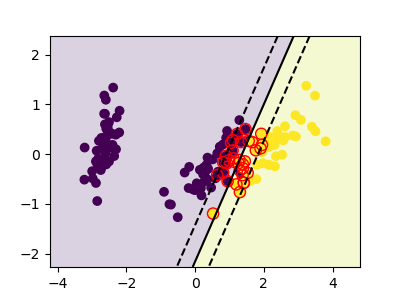
\includegraphics[width=0.5\linewidth]{graphics/svm_classifier_violation.png}
    \caption{A soft svm classifier has been trained to detect one of the classes in the \texttt{iris} dataset (yellow). We have trained it on the top-2-scores resulting from a PCA, to be able to easily visualize it. Shown is the optimal separating hyperplanes, as well as the support vectors (marked with red boundaries), and the lines $\sprod{\beta^*,x_i}=\pm 1$. Notice that the support vectors here are not necessarily vectors with $\sprod{\beta^*,x_i}=\pm 1$. Best viewed in color. }
    \label{fig:svm_soft}
\end{figure}
\subsection{Non-linear SVM:s and the kernel trick}
We have already remarked that linear decision boundaries are not always the best idea -- many datasets do not have a geometry that admits linear decision boundaries. What can we do in that case?

The first idea is to simply transform the features $x_i$ to $\varphi(x_i)$ using some non-linear map $\varphi: \R^p \to \R^d$, and then train an SVM using $\varphi(x_i)$ as the data points. One can for instance calculate all products $(x_ix_j)_{i,j}$, or even higher polynomial terms. This can definitely work-- if we choose the map $\varphi$ correctly, the transformed data can be linearly separable, although the non-transformed is not.  An example of this is given in Figure \ref{fig:polar}.

\begin{figure}
    \centering
    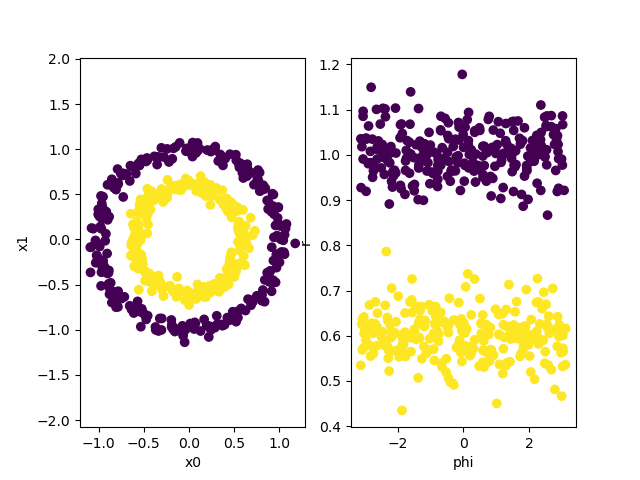
\includegraphics[width=0.5\linewidth]{graphics/polar.png}
    \caption{The left dataset is not linearly separable. If we transform it into polar coordinates, it however is.}
    \label{fig:polar}
\end{figure}

This approach has two major drawbacks
\begin{itemize}
    \item It is hard to a priori choose the transformation $\varphi$. For high-dimensional data, it is very unlikely that we can 'see' the correct geometry such as in the example in Figure  \ref{fig:polar}.
    \item $\varphi$ will typically increase the dimension of the data, and therefore also the size of the $\beta$, which makes the computational burden a lot higher.
\end{itemize}
Fortunately, there is a very elegant trick that implicitly incerts a non-linearity $\varphi$ -- the so-called \emph{kernel trick}. To understand it, let us have a look at the dual problem when feeding it with $\varphi(x_i)$ instead of $x_i$.
\begin{align*}
        \sup_{\gamma \geq 0} \sum_{i \in [n]}\gamma_i -\tfrac{1}{2} \norm{\sum_{i\in [n]}\gamma_i y_i \varphi(x_i)}_2^2 = \sup_{\gamma \geq 0 }  \sum_{i \in [n]}\gamma_i -\tfrac{1}{2} \sum_{i,j\in [n]}\gamma_i\gamma_j y_iy_j \sprod{\varphi(x_i),\varphi(x_j)}
    \end{align*}
    We notice two things: First, the dual problem will have the same computational burden regardless of the choice of $\varphi$. Secondly, the solution only depends on the values of $\sprod{\varphi(x_i),\varphi(x_j)}$. If we write these as $K(x_i,x_j)$ for some non-linear function $K$, we obtain the \emph{dual kernel SVM} problem
    \begin{align}
        \sup_{\gamma \geq 0 }  \sum_{i \in [n]}\gamma_i -\tfrac{1}{2} \sum_{i,j\in [n]}\gamma_i\gamma_j y_iy_j K(x_i,x_j). \label{eq:kernelsvm}
    \end{align}
    The primal solution $\beta_*$ can directly be calculated from the dual solution:
    \begin{align*}
        \beta_* = \sum_{i \in [n]} \gamma_i^*y_i \varphi(x_i).
    \end{align*}
    This cannot be determined without knowledge of $\varphi$. However, and this is the gist, its classifications can!
    \begin{align}
        \sprod{\beta_*,\varphi(x)} =\sum_{i \in [n]} \gamma_i^*y_i \sprod{\varphi(x_i),\varphi(x)} =  \sum_{i \in [n]} \gamma_i^*y_i K(x_i,x) \label{eq:kernelclass}
    \end{align}
So \emph{all calculations} can be made without explicitly knowing the non-linear transformation $\varphi$!

The formula \eqref{eq:kernelclass} reveals an interesting interpretation of the Kernel SVM: For each new example, we calculate a weighted average of the labels of the training data. The weights are determined by $\gamma_i^*$, which is only non-zero for the support vectors, and the values of $K(x_i,x)$. The bigger $K(x_i,x)$, the higher the influence of the label of $x_i$ on the classification of $x$. Therefore, we should think about $K(x,y)$ as a \emph{similarity measure} of the data-points $x$ and $y$.

Two examples of kernels:
\begin{itemize}
    \item Polynomial kernels: $K(x,y) = (1+\gamma\sprod{x,y})^d$, with tuneable $\gamma>0$ and $d$. Using the kernel of degree $d$ corresponds to using a $\varphi$ calculating all products $\Pi_k x(k)^{n_k}$ for $\sum_{k}n_k \leq d$.
    \item Radial basis kernel (rbf kernel):  $K(x,y) = e^{-\gamma\norm{x-y}^2}$ for a tuneable parameter $\gamma>0$. Here, the intuition for the corresponding $\varphi$ is less immediate.
\end{itemize}

Can we use any $K$ as a valid kernel function? In principle yes. But if we want to preserve the interpretation of \label{eq:kernelsvm} as the dual of a linear SVM applied to non-linearly transformed features, we need to be a bit careful.

\begin{defi}
    Let $X$ be a set. A function $K:X \times X\to \R$ is  \emph{positive definite}, or a \emph{Kernel function}, if for each choice of points $(x_i)_{i\in [N]}$ (for arbitrary $N$), the matrix $(K(x_i,x_j))_{i,j\in [N]}$ is symmetric positive semi-definite.
\end{defi}

\paragraph{Example} A trivial example of a kernel is $K(x,y)=\sprod{x,y}$. We namely have for $x_i$ and $c_i$ arbitrary
\begin{align*}
    \sprod{c, (K(x_i,x_j))_{i,j} c} = \sum_{i,j} c_ic_j \sprod{x_i,x_j} = \sprod{\sum_i c_i x_i, \sum_i c_i x_i} = \norm{ \sum_i c_i x_i}_2 \geq 0
\end{align*}

The following remarkable theorem holds.
\begin{theorem}
    The following are equivalent.
    \begin{enumerate}[(i)]
        \item $K$ is a Kernel function.
        \item There exists a Hilbert space $\calH$ and a feature map $\varphi: x\to \calH$ so that $K(x,y) = \sprod{\varphi(x),\varphi(y)}_{\calH}$.
    \end{enumerate}
\end{theorem}
\begin{proof}
    To prove (i)$\implies$(ii) is relatively simple: We need to prove that for arbitrary $c\in \R^n$
    \begin{align*}
        \sum_{i,j\in [N]} c_ic_j K(x_i,x_j) \geq 0.
    \end{align*}
    But
    \begin{align*}
        \sum_{i,j \in [N]} c_ic_j K(x_i,x_j) &=   \sum_{i,j \in [N]} c_ic_j\sprod{\varphi(x_i),\varphi(x_j)} = \sprod{\sum_{i\in [N]}c_i \varphi(x_i),\sum_{i\in [N]}c_i \varphi(x_i)}_\calH \\
        &= \norm{\sum_{i\in [N]}c_i \varphi(x_i)}_\calH^2\geq 0
    \end{align*}
    To prove the other direction is considerably harder -- we will not do it here.
\end{proof}

Let us prove that a theorem that lets us construct a lot of kernels, and in particular see that the examples we quoted above really are kernels.
\begin{theorem}
    Assume that $K$, $L$ and $(M_n)_{n\in N}$ are kernel functions. Then the following functions also are:
    \begin{itemize}
        \item $aK + bL, a,b\geq 0$,
        \item $M=\lim_{n\to \infty}K_n$, if the limit (pointwise),
        \item $K_f(x,y)=f(x)K(x,y)f(y)$ for $f : X\to \R$ is an arbitrary function,
        \item $KL$.
    \end{itemize}
\end{theorem}
\begin{proof}
    The first two statements are quite easy to prove -- if $c$ and $(x_i)$ are arbitrary, we have
    \begin{align*}
        \sum_{i,j} c_ic_j (aK(x_i,x_j)+bL(x_i,x_j)) &=  a\underbrace{\sum_{i,j} c_ic_j K(x_i,x_j)}_{\geq 0}+b\underbrace{\sum_{i,j} c_ic_j L (x_i,x_j) \geq 0}_{\geq 0} \\
         \sum_{i,j} c_ic_j M(x_i,x_j) &= \lim_{n\to \infty }  \sum_{i,j} c_ic_j M_n(x_i,x_j) \geq \lim_{n\to \infty} 0 = 0. \\
         \sum_{i,j} c_ic_j f(x_i)K(x_i,x_j)f(x_j) &= \sum_{i,j}(c_if(x_i))(c_jf(x_j))K(x_i,x_j) \geq 0 
    \end{align*}
    The last statement is a lot trickier. Since $\kappa =(K(x_i,x_j))_{i,j}$ and $\lambda =(L(x_i,x_j))_{i,j}$ are symmetric and positive, we can write $\kappa = A^*A$ and $\lambda = B^*B$ for some $A$ and $B$. If we let $A^i$ and $B^j$ denote the columns of $A$ and $B$, respectively, this implies
    \begin{align*}
        (\lambda \cdot \kappa)_{i,j} = \sprod{A^i,A^j}\sprod{B^i,B^j} =  \sum_{k,\ell} A^i_kB^i_\ell A^j_kB^j_\ell.
    \end{align*}
    If we define the vectors $C^i$ through $C^i_{kn+\ell}=A^i_kB^i_\ell$, what we have shown above is that 
    \begin{align*}
        (\lambda \cdot \kappa)_{i,j} = \sprod{C^i,C^j},
    \end{align*}
    i.e. $\lambda \cdot \kappa = C^*C$, i.e. that $\lambda \cdot \kappa$ is positive semidefinite.
\end{proof}
We can now argue that $(1+\gamma\sprod{x,y})$ is a kernel function as a positive linear combination of two kernel functions, and then $(1+\gamma\sprod{x,y})^d$ as a product of kernel functions. As for $\exp(-\gamma \norm{x-y}_2^2)$, we have
\begin{align*}
   \exp(-\gamma \norm{x-y}_2^2) = \exp(-\gamma\norm{x}_2^2) \exp(2\gamma \sprod{x,y})\exp(-\gamma \norm{y}_2^2).
\end{align*}
By our theorem, it is hence enough to prove that $K(x,y) =\exp(2\gamma \sprod{x,y})$ is a kernel function. However,
\begin{align*}
    \exp(2\gamma \sprod{x,y}) = \lim_{n\to \infty} \sum_{k=0}^n \frac{\sprod{x,y}^k}{k!}
\end{align*}
is a limit of positive linear combinations of kernel functions, i.e., a kernel function.

\paragraph{The feature space of the rbf kernel} We mentioned that the polynomial kernel can be realized through of a polynomial map $\varphi$. What about the rbf kernel? We know that there exists a $\calH$ and a map $\varphi:\R^p\to \calH$ so that $\exp(-\gamma\norm{x-y}_2^2)= \sprod{\varphi(x),\varphi(y)}$. This map is not as simple to imagine -- in fact, one can prove that $\calH$ must have infinite dimension. We include the proof of this for completeness -- but it is surely goes beyond the scope of this course.

\begin{theorem}
    If $\calH$ is a Hilbert space so that there exists a map $\varphi:\R^p\to \calH$ is a map with $\sprod{\varphi(x),\varphi(y)} = \exp(-\gamma \norm{x-y}_2^2)$ for all $x,y$, $\calH$ has infinite dimension.
\end{theorem}
\begin{proof}
    We will show that the unit ball in $\calH$ is not compact, which implies that $\calH$ must have infinite dimension by the Heine Borel theorem (the unit ball in every finite-dimensional space is compact). Consider the infinite set $\varphi(x), x\in \Z^p$. All these elements have unit norm, since $\norm{\varphi(x)}_2^2=\sprod{\varphi(x),\varphi(x)}=\exp(-\gamma \norm{x-x}_2^2)=1$. Also
    \begin{align*}
        \norm{\varphi(x)-\varphi(y)}_2^2 = \norm{\varphi(x)}_2^2+\norm{\varphi(y)}_2^2 - 2\sprod{\varphi(x),\varphi(y)} = 2 - 2\exp(-\gamma\norm{x-y}^2)\geq 2(1-e^{-\gamma})>0
    \end{align*}
    since any two $x,y\in \Z^p$ are separated by a distance of at least one. But if the unit ball was compact, we would be able to find a limit point in the set $(\varphi(x))_{x\in \Z^p}$ -- this is a contradiction to the fact that any two elements in the set are separated by at least $2(1-e^{-\gamma})>0$.
\end{proof}


\subsection{Further reading and recommended exercises}

Support vector machines are treated in Chapter 9 of An Introduction to Statistical Learning. For those who want more information about the theory of convex optimization, we recommend the excellent book \cite{boyd2004convex}. The concept of duality in convex optimization is in particular discussed in Chapter 5 of the latter.

Recommended exercises in An Introduction to Statistical Learning are 9.7.2 and 9.7.3. Consider also the following exercises.

\begin{exercise}
    Derive the form of the dual problem of the Soft Margin SVM.
\end{exercise}

\begin{exercise}
    (i) (\emph{Algebra-heavy}) Consider the following version of Ridge regression
    \begin{align*}
        \min_{\beta} \tfrac{1}{2}\norm{X\beta-Y}_2^2 \text{ subject to } \norm{\beta}_2^2 \leq s.
    \end{align*}
    Show that the dual of this problem is
    \begin{align*}
        \sup_{\gamma \geq 0 } \sprod{(\id - X(X^*X+\gamma)^{-1}X^*)Y,Y} -\gamma s.
    \end{align*}

    (ii) \emph{Challenging}. Show that there exists an $s_0$ so that the solution of the dual problem is equal to $\gamma=0$ for all $s\geq s_0$. Show that if $X$ has full rank, this $s_0$ is equal to the square of the norm of the smallest-norm solution of $X\beta=Y$.
\end{exercise}

\begin{exercise}
    Explain why $K(x,y) = \sprod{x,y}$ is referred to as the \emph{linear kernel}.
\end{exercise}

\begin{exercise}
    (\emph{Challenging}) Use the dual form of the SVM problem to argue that the solution $\beta^*$ of it is the vector in the \emph{convex hull} of the vectors $x_iy_i \in \R^p, i\in[n]$ that is closest to the origin. 
    
    The convex hull of the $x_iy_i$ is thereby the set of vectors that can be formed as weighed averages of them, i.e
    \begin{align*}
        \{ \sum_{i \in [n]} \theta_i x_iy_i \, \vert \sum_{i\in [n]} \theta_i= 1, \theta_i \geq 0 \}
    \end{align*}
    \emph{Hint}: Show that the dual-optimal $\gamma^*$ must fulfill $\sum_i \gamma_i^*=1$, by studying how scaling of $\gamma$ affects the function that is optimized in the dual problem.
\end{exercise}

\begin{exercise}
    Let $f: \R^p\to \R$ be a function. Show that $K(x,y)=f(x)f(y)$ is a kernel function.
\end{exercise}

\begin{exercise}
    Show that $f(x,y) = \norm{x-y}$ is \emph{not} a kernel function.
\end{exercise}





\section{Decision trees}
Any classification method will ultimately divide the data space $\R^p$ into distinct regions $C_k$, $k\in[K]$, and then assign the examples in $C_k$ to the class $k$.  \emph{Decision trees} is a simple and interpret able way to construct such regions. Let's begin by describing a decision tree, and  worry about how to build good ones later.\footnote{We will here solely focus on trees for classification problems. One can also apply tree-based methods for regression -- that leads to so-called \emph{regression trees}. We defer to \cite{james2023introduction} for more information on that.}

A decision tree is a tree in a graph sense -- i.e., it is a graph without cycles. In other words, it can be seen as a directed graph with a 'mother-node', which is connected to children, which themselves have children and so forth. The nodes without children are called \emph{leaves}. To classify an example, we traverse the tree from the 'mother node' down to a leave. In each node, we have a criterium to decide which node to choose.

\paragraph{Example} A simple example would be the decision tree "Should I bring an umbrella?". In the mother node, I check whether it is raining outside. If it does, I to a leaf directly which says 'Yes'. If not, I continue to a new node. There, I check whether it might rain later. If yes, I go to a leaf which says 'Yes'. If no, I go to a leaf which says 'No'. See Figure \ref{fig:Tree}. \newline

    \begin{figure}
        \centering
        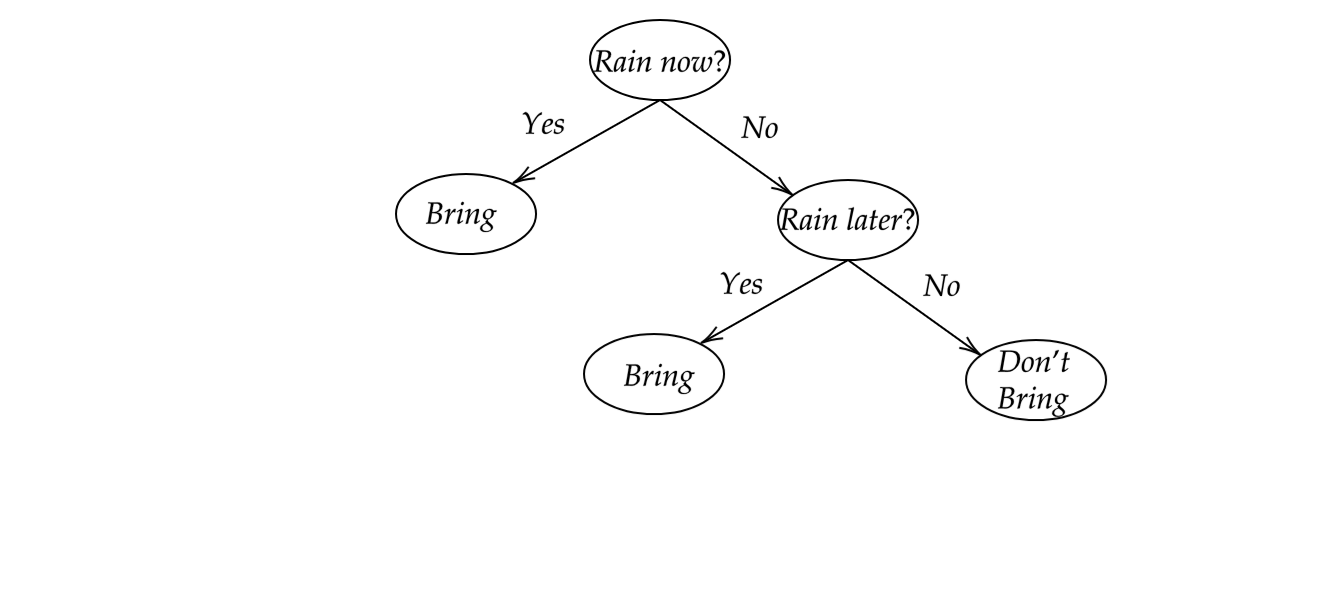
\includegraphics[width=0.5\linewidth]{decision_tree.png}
        \caption{A simple decision tree for deciding whether to bring an umbrella.}
        \label{fig:Tree}
    \end{figure}


In a statistical  learning setting, we need to make decisions based on the value of the features $x(\ell)$. The features can be both of qualitative nature ('Does it rain?') or quantitative nature ('is $x(\ell)>s^*$?').  In a decision tree, we only choose one feature per node -- this is by design. Only allowing for single feature decision makes it simpler to find the 'most effective' decision -- and leads to a more interpretable model after the fit. 

Fitting the tree is now done in a greedy fashion. We initialize a tree with a single node, where all examples land. We then go through all possible decisions (all features and all threshold) and chooses the one that \emph{decreases the impurity} the most -- that is, puts the resulting distribution of training data 'closest' to a tree with only leaves only containing a single class (pure leaves). We'll look at some concrete impurity measures later.


The resulting algorithm is conceptualised in Algorithm \ref{alg:decision_build}.

Equation \eqref{eq:impurity_drop} looks complicated, but this is just a notational issue. In words, again, we 'try' all possible new splits, and measure the weighted average of the impurity in the potential resulting nodes. The split that causes the biggest drop in impurity is chosen.

We can choose different stopping criteria. Some possible are limiting the depth of the trees, requiring a minimal amount of samples in each leaves, or stopping when the impurity drop gets smaller than some tolerance.

\begin{algorithm}[tb]      
	\caption{Building a decision tree} 
	\begin{algorithmic} [1]
 		\REQUIRE Training data $X$, labels $Y$, impurity measure $I$.\label{alg:decision_build}
 		\STATE $T_0=$ Tree with a single node containing all data.
 		\REPEAT
            \FOR{ Leafs $\ell$ in $T_k$ }
                \STATE Determine the feature index $k^*$ and the threshold $s_{k^*}$ so that
                \begin{align}
                    \Delta_{\ell,k} = \abs{\ell} I(\ell)  - \left(\abs{\{\ell, x_k>s\}} I(\ell, x_k>s) + \abs{\{\ell, x_k\leq s\}} I(\{\ell, x_k\leq s\})\right) \label{eq:impurity_drop}
                \end{align}
                is as small as possible.
                \STATE $\Delta_\ell = \Delta_{\ell,k^*}$
            \ENDFOR
            \STATE Split the leaf $\ell$ according to the criterion $x_{k^*}\leq s_{k^*}$ that has the highest value of $\Delta_{\ell,k^*}$
 		\UNTIL stopping criterion is met at $k= k_*$
 		\RETURN $T_k$
	\end{algorithmic}
\end{algorithm}

\subsection{Impurity measures} How should we measure the impurity of a node? We are interested in how \emph{uniform} the distribution of the class indices $y$ within the subset of data contained in a node. Since this distribution can be interpreted as a probability distribution, we might as well speak about the the impurity of a \emph{probability distribution}.

\paragraph{Error rate} A very crude measure is simply to measure the probability of the most probable class. The closer this is to $1$, the more uniform the distribution is. The impurity measure is thus
\begin{align*}
    1 - \max_k \mathbb{P}(y=k).
\end{align*}
This is however too crude -- it will for instance not differentiate between distributions where all examples belong to one of two classes (with equal probability) or a distribution where half of the examples belong to one class, and the others are uniformly distributed between the rest. The latter is intuitively much less uniform (or to put it algoritmically, will lead to a harder situation after splitting off the big class).

\paragraph{Gini impurity} The Gini-impurity index is defined as the probability that a randomly drawn example from the distribution is misclassified, if we assign an index to it randomly to the distribution. In formulas, this becomes
\begin{align*}
    \sum_{k \in [K]} \mathbb{P}(Y=k)(1-\mathbb{P}(Y=k)).
\end{align*}
The probability of an element with class $k$ to be misclassified when using the random label is $\mathbb{P}(Y\neq k)=1-\mathbb{P}(Y=k)$ -- and the probability of drawing such an element is $\mathbb{P}(k)$.

\paragraph{Shannon entropy} The entropy of a probability distribution is defined as 
\begin{align*}
    \sum_{k \in [K]} -\mathbb{P}(Y=k)\log_2(\mathbb{P}(Y=k)).
\end{align*}
with the convection that $0\log(0) :=\lim_{x\to 0^+}x\log(x)=0$.

This definition stems from information theory. Roughly, the motivation is as follows: If we want to be able to send $2^N$ messages using zeros and ones, we need $N$ zeros and ones -- and if all are equally likely, we will need $N$ such \emph{bits} of information. Hence, we can interpret each event -- with probability $2^{-N}$-- as containing $N$ bits of information. Generalizing this, we see that an event of probability $p$ contains $-\log_2(p)$ bits of information -- the entropy is hence the \emph{expected information content} of observing a sample in the distribution.


One can show that entropy is minimized (equal to zero) when $\mathbb{P}(Y=k)=1$ for some $k$, and maximized (on the set of probability distributions on $K$ classes) when all labels are equally probable. Hence, a low entropy is a good indicator of a uniform distribution of labels.

\subsection{Stopping criteria}
When should we stop fitting the tree? We could in principle keep splitting the tree until each node only contains one datum. This is however not wise -- this strategy is very prone to overfitting. Instead, we should stop at a point where the tree is not too complicated, but still separates the training data into nodes with quite low impurity. Here are a few examples of stopping criteria to use:
\begin{itemize}
    \item Maximum depth: Only allow splitting up to a pre-determined depth.
    \item Leaf size: Stop splitting when the leaves are small enough.
    \item Number of leaves: Stop when the trees has a certain number of leaves (which corresponds to a certain number of 'decision paths').
    \item Minimal impurity decrease: Stop when splitting the tree will not lead to a high enough decrease in impurity.
\end{itemize}

\subsection{Ensemble learning}
Decision trees are great in that they are relatively interpretable, extremely versatile and simple to train. However, they suffer from a very \textbf{high variance} -- small changes to the training set can lead to extreme changes (potentially, changing one training example could lead to a different first split, which completely changes the structure of the tree). How to mitigate this?

\begin{figure}
    \centering
    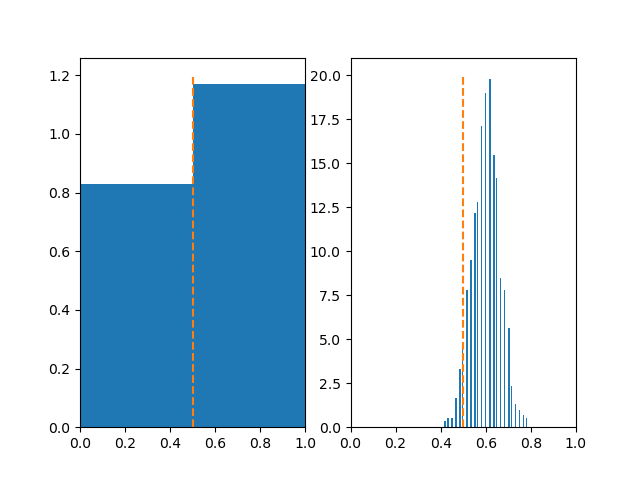
\includegraphics[width=0.6\linewidth]{graphics/ensemble_example.png}
\caption{A single learner only has to be correct a little more than half of the time for the majority a collective independent copies of it to be correct quite often.}
\label{fig:ensemble}
\end{figure}

A strategy which is surprisingly effective is to train more than one tree, and let them work together. To intutively understand this, image a group of $N$ persons trying to decide whether mushrooms are poisonous or not. Every single person is not that good at the task, and succeed only in $60\%$ of the cases. However, if we let them each guess \emph{independent from each other}, the number of correct answers will for $N$ large very likely be more than the correct answers. Hence, \textbf{an ensemble of weak, independent models} will as a collective \textbf{be strong}. See Figure \ref{fig:ensemble}.



Let's now  first discuss two concrete methods to achive the ensemble effect --\emph{bagging} and \emph{random forests} --  before we go on to looking at \emph{ensembling methods} in general.










\begin{figure}
    \centering
    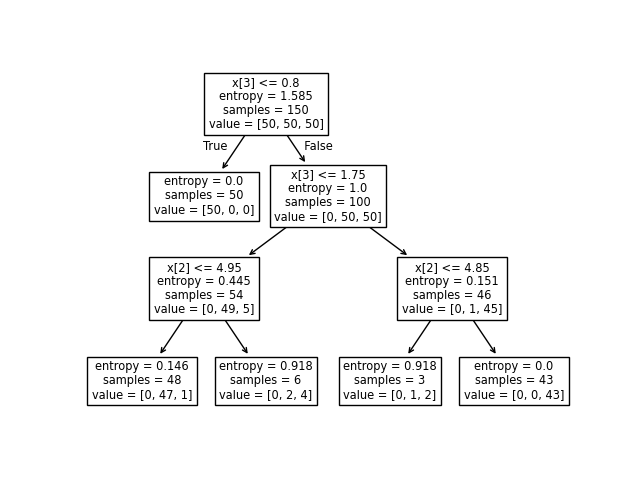
\includegraphics[width=0.35\linewidth]{graphics/trained_tree.png}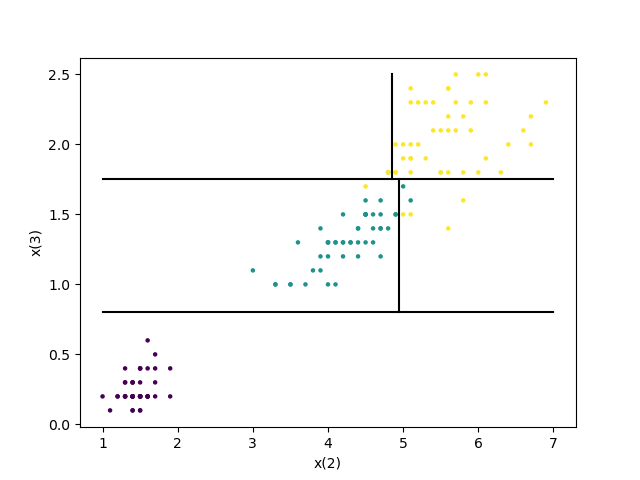
\includegraphics[width=0.35\linewidth]{graphics/decision_surfaces.png}
    \caption{Left: A decision tree, trained on the IRIS dataset. Right: The corresponding decision boundaries.}
    \label{fig:enter-label}
\end{figure}


\subsubsection{Bagging}
Bagging is a shorthand for \emph{Bootstrap AGgregating}. When bagging, we train $N>1$ small trees. Each tree can only access a bootstrapped sample of the data, i.e. drawn with replacement. To achieve the independence of the learners, the bootstrap draws are drawn independently. This will not lead to perfectly independent learners -- many of them will look at the same examples -- but it should at least hold approximately.


\subsubsection{Random forests} Another tree ensemble method is \emph{random forests}. We again use a multitude of decision trees ($=$ a 'forest') that we train (most often via bagging, but this is not theoretically needed). We however achieve the independence in another way: Each learner now is only allowed to use a \text{random subset} of the features! (In some implementations, one chooses this subset at each split).

The rationale behind this strategy can be best explained if we assume that the features are independent. Then, two trees looking at different subsets will be independent, and our ensembling idea will work. In practice, assuming that the features  are independent is of course very unrealistic, and one should rather view the trees as \emph{decorrelated} than indepedent. Still, this is enough to increase performance in many practical scenarios.  

An even more handwavy argument is that using a random forest helps to \emph{diversify} the trees. If there is one predictor that is very likely to make a good initial split regardless of the draw of the data, all trees in a bagged ensemble will probably make that split. It could however be that making other splits first leads to a better final tree in the end -- the decision tree building algorithm is \emph{greedy}. In a random forests, there will be trees having to avoid the 'canonical' first split, making it forced to explore other alternatives.


\begin{figure}
    \centering
    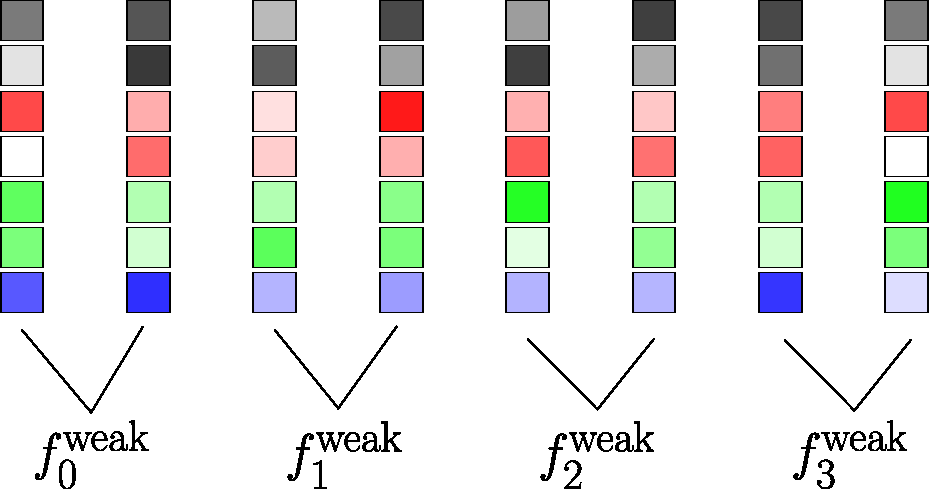
\includegraphics[height=2cm]{graphics/bagging.pdf}\hspace{3cm}\hspace{-1cm}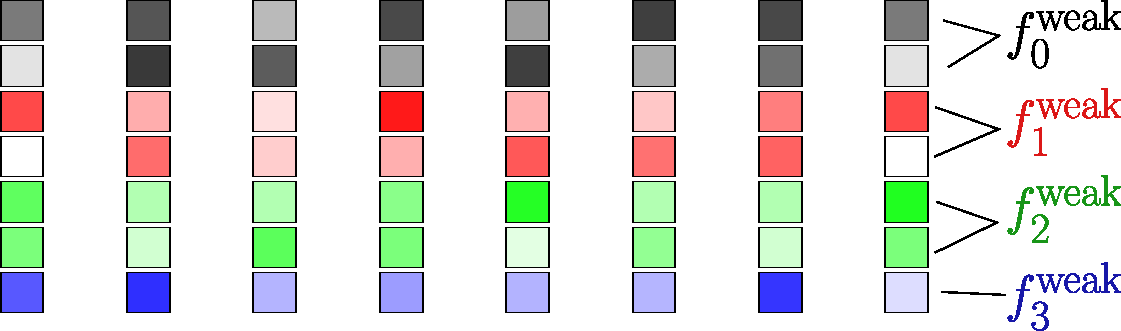
\includegraphics[height=1.5cm]{graphics/boosting.pdf}
    \caption{Simplified illustrations of the ideas of bagging and random forests. In bagging, each model can only look at a subset of the data. In random forests, each model can only look at a subset of the features. (Note that the two methods are not exclusive)}
    \label{fig:bagging_random_forests}
\end{figure}

\subsubsection{The 'ensemble learning theorem'
}
Let us formalize our ideas from above in general. Let $(f_i^{\mathrm{weak}})_{i\in [N]}$ be a set of classifiers (weak learners). Ensembling them refers to training them individually and then using the average as our classifier:
\begin{align} \label{eq:ensemble}
    f(x) = \frac{1}{N}\sum_{i\in [N]}f_i^{\mathrm{weak}}(x).
\end{align}
One should note that in the classification example, the class with the highest probability in \eqref{eq:ensemble} will be the same as the class that is chosen by the most classifiers, i.e. the 'winner' in a majority vote.

The following simple but far-reaching theorem holds.
\begin{theorem} \label{th:ensemble}
    Assume that $N$ weak classifiers $f_i^{\mathrm{weak}}$ are , and trained on \textbf{independent and identically distributed data}. Let $b^{\mathrm{weak}}$ and $v^{\mathrm{weak}}$ denote the common values of the bias and variance of the weak classifiers. Then, the bias $b$ and variance $v$ of the ensemble 
    \begin{align*}
        f = \frac{1}{N} \sum_{i \in [N]}f_i^{\mathrm{weak}}
    \end{align*}
    are given by
    \begin{align*}
        b = b^{\mathrm{weak}}, \quad v = \frac{1}{N}v^{\mathrm{weak}}.
    \end{align*}
\end{theorem}
\begin{proof}
    We have 
\begin{align*}
   \erw_D(f(x)) = \frac{1}{N}\sum_{i\in [N]}\erw_D(f_i^{\mathrm{weak}}(x)) = \erw_D(f^{\mathrm{weak}}(x)).
\end{align*}
Hence, on average, the estimate of the ensemble is the same as the average of each weak learner -- and consequently, also the bias. As for the variance, the indepedence of the data fed into the weak learners imply that $f_i^\mathrm{weak}(x)$ are independent, so that
\begin{align*}
    \mathbb{V}_D(f(x)) = \sum_{i\in [N]}\mathbb{V}_D(\tfrac{1}{N}f_i^{\mathrm{weak}}(x)) = \frac{1}{N^2} \cdot N v(x) = \frac{1}{N}v(x).
\end{align*}
Taking the expected value over $x$ yields the claim.
\end{proof}
Theorem \ref{th:ensemble} seems almost too good to be true: we can basically reduce the variance for free! There is however no free lunch: Note that in order to train $N$ \emph{independent} classifiers, we need $N$ times \textbf{more computing power}, and also $N$ times \textbf{more data}! (Note that using little data for each weak classifier will increase their variance). In practice, we therefore often use strategies where the individual learners are not independent in the strict sense, but still quite uncorrelated, such as bagging and random forests.

\paragraph{Variable importance} An ensemble classifier resulting hundreds or even thousands of trees is much \textbf{less interpretable} than a single tree. There are methods to still measure the importance of features, for instance via recording the total decrease of impurity caused from splits over each feature in each tree, averaged over the tree. If a feature is used in many trees to perform many 'decisive' splits, it should be important.

\subsection{Boosting} Boosting is a class of methods also where the main idea is to combine many weak learners to produce a better performing ensemble. The method is however \emph{fundamentally different} to bagging and random forests in that the weak learners are trained \emph{sequentially}. We train a first weak learner (on all the data), and record the errors that it makes. We then train a second weak learner to \emph{correct} those errors, record a new set of errors, train a new weak learner to correct those, and so forth. Combining all the weak learners, that 'correct each others errors', should in the end lead to a very accurate classifier.

Note that in contrast to random forests and bagged ensembles, the weak learners in a boosting application are \textbf{not independent}. Theorem \ref{th:ensemble} is therefore not applicable -- indeed, boosting will in general \textbf{not} lead to \textbf{reduced variance}. Instead, the idea here is to use weak, inflexible learners each with a very small variance but combine them to \textbf{reduce bias}. \newline

There are many different algorithm referred to as 'boosting'. We will here concentrate on a particular one called \textbf{ADABoost} (ADAptive Boosting). We will also restrict ourselves to the case of two classes $y=1$ and $y=-1$. 

\paragraph{Basic idea} In ADABoost, we iteratively assign \emph{weights} $w_k^i$ to the training examples -- the higher the weight, the more important that training example is. Note that we can train a decision tree just as before with weighted samples -- the only difference is that we in \eqref{eq:impurity_drop} need to use the total weights of the new leaves instead of the relative fraction of samples, i.e.
\begin{align*}
    \sum_{k: x_k \in \ell, x_k>s}w_k^iI(\ell)  - \left(\left(\sum_{k: x_k \in \ell, x_k>s}w_k^i\right) I(\ell, x_k>s) + \left(\sum_{k: x_k \in \ell, x_k\leq s}w_k^i\right) I(\ell, x_k\leq s)\right),
\end{align*}
to prioritize making good splits involving important samples. The original algorithm does exactly this when all samples have equal weights -- this is also how we initalize our algorithm. Note that many other algorithms can be formulated with weights on the sample this ways, making it plausible that ADABoost principle is very general. Another alternative is to, in each step, simply bootstrap a training sample using (normalized) weights as sample probabilities, and then train it as usual.

We also assign another set of weights $\alpha_m$ to the \emph{classifiers}. If the single classifiers are called $f_i^\weak$ (outputting either $1$ or $-1$ for each training example), the  classifier we use after $m$ steps is
\begin{align*}
    f^m = \sgn\left(\sum_{i=0}^m \alpha_i f_i^\weak\right).
\end{align*}
That is, we decide on a classification using a \emph{weighted} majority vote -- the more confident we are in $f_i^\weak$, the higher is $\alpha_i$.

\paragraph{Derivation of weights and weak classifiers} Suppose that we have constructed the first $m$ classifiers and weights. How should we choose $\alpha_m$ and $f_m^\weak$? The strategy of ADABoost is to choose them to minimize the \emph{exponential loss}
\begin{align} \label{eq:err}
    E = \sum_{i\in[n]} e^{-y_if^m(x_i)}
\end{align}
What minimizing $E$ means is clear -- if $y_i=1$, $f_m(x_i)$ should be as large as possible, and if $y_i=-1$, it should be as negative as possible -- this is exactly what we want from the classifier $f^m$!\footnote{There is  more sophisticated ways to motivate the use of an exponential loss, related to the fact that the $y_i$ are binary  -- see \cite[Chapter 10]{hastie2009elements}.} \newline

We can rewrite $E$ as follows
\begin{align*}
     E= \sum_{i\in[n]} e^{-y_if^m(x_i)} = \sum_{i\in [n]}e^{-y_if^{m-1}(x_i)} \cdot e^{-y_i\alpha_m f_m^{\weak}(x_i)}:= \sum_{i\in [n]}w_i^m \cdot e^{-y_i\alpha_m f_m^{\weak}(x_i)},
\end{align*}
where we \emph{defined} the weights
\begin{align} \label{eq:weights}
    w_i^m = e^{-y_if^{m-1}(x_i)}.
\end{align}
These will be small if $f^{m-1}(x_i)y_i$ is positive, i.e. when $f^{m-1}(x_i)$ is correct, and big otherwise. Hence, in this way, we make the new weak learner \emph{concentrate on the examples $f^{m-1}$ misclassify}!

Since $f^\weak_m(x_i)$ only take on the values $1$ and $-1$, as is $y_i$, we can rewrite $E$ even more:
\begin{align*}
    E= \sum_{i : y_i = f_m^\weak(x_i)}w_i^m e^{-\alpha_m} + \sum_{i : y_i \neq f_m^\weak(x_i)}w_i^m e^{\alpha_m} 
\end{align*}
Letting $W_c= \sum_{i : y_i = f_m^\weak(x_i)}w_i^m$ be the total weight of the by $f_m^\weak$ correctly classified examples and $W_e =  \sum_{i : y_i \leq f_m^\weak(x_i)}w_i^m$ the weight of the incorrectly classified ones, we hence have
\begin{align} \label{eq:error}
    E = e^{-\alpha_m} W_c + e^{\alpha_m}W_e
\end{align}
We see that \emph{for every $\alpha_m>0$}, we reduce $E$ the most if we simply minimize the weighted error $W_e$ -- since $W_e+W_c$ is just the total weight, and . Hence, we define
\begin{align} \label{eq:weak tree}
    f_m^\weak(x_i) = \text{ Tree fitted using sample weights $w_i^m$.}
\end{align}
The attentative reader might have noticed that decision trees actually do not minimize the weighted error, but instead use the Gini or entropy errors to build the 'best' trees. This works better in practice, but is no problem for the algorithm -- it might not be the greedily best thing we can do in theory, but we do not have to.

Once we have determined the next weak classifier, we need to assign the weight $w_m$. Here, we can analytically determine the optimal weight to use through minimizing \eqref{eq:error}. One obtains
%\begin{align*}
%    0 = \frac{\partial}{\partial \alpha_m} E = -e^{-\alpha_m} W_c + e^{\alpha_m}W_e,
%\end{align*}
%which one quickly juggles to
\begin{align} \label{eq:optimal_alpha}
    \alpha_m = \frac{1}{2}\ln\left(\frac{W_c}{W_e}\right) = \frac{1}{2}\ln\left(\frac{1-e}{e}\right),
\end{align}
where we defined $e=W_e/(W_e+W_c)\in [0,1]$ as the \emph{weighted error rate}. Here we can remark that the closer $e$ is to $0$, the higher we set the weight -- the better the weak lerner, the more confident we are in it. 

\paragraph{Remark:} One should remark that if $e>\tfrac{1}{2}$, the optimal weight $\alpha_m$ is negative. We however assumed that $\alpha_m>0$ when defining $f_m^\weak$. That is however not a problem -- if $e>\tfrac{1}{2}$, the weak classifier is actually \emph{worse} than flipping a coin. We hence should do the opposite of what it is saying, and we are also: $\alpha_mf_m^\weak$ is moving the classification $f^m$ in the opposite direction to what $f_m^\weak$ saying.

This technicality is related to the original motivation of boosting -- answering the \emph{theoretical} question if weak learners can be combined to strong ones. The above derivation can be used to argue that as long that the weak \emph{always} puts out a weighted error rate $e$ strictly smaller than $\tfrac{1}{2}$ (i.e. are guaranteed to be just a bit better than flipping a coin), the ensemble will ultimately succeed. \newline

Let us end this section by summarizing AdaBoost in \eqref{alg:adaboost}. Note that the weight update step is justified by the fact that  \eqref{eq:weights} and the definition of $f^m$ implies 
\begin{align*}
    w_i^{m+1} =e^{-y_if^{m}(x_i)} = e^{-y_i(f^{m-1}(x_i)+\alpha_mf_m^\weak(x_i))} = w_i^m \cdot e^{-\alpha_m y_if_m^\weak (x_i)}.
\end{align*}

\begin{algorithm}[tb]      
	\caption{AdaBoost for binary classification trees} 
	\label{alg:adaboost}
	\begin{algorithmic} [1]
 		\REQUIRE Training data $x_i$, labels $y_i \in \set{-1,1}$, $i\in [n]$.
 		\STATE $f^0=0$, $w_i^0 = \tfrac{1}{n}$.
 		\REPEAT
 			\STATE Fit a tree $f_m^\weak$ with the sample weights $w_i^{m}$.
            \STATE Let $e$ be the weighted error rate of $f_m^\weak$ and set 
            \begin{align*}
                \alpha_m =  \frac{1}{2}\ln\left(\frac{W_c}{W_e}\right) = \frac{1}{2}\ln\left(\frac{1-e}{e}\right)
            \end{align*}
            \STATE Update the classifier
            \begin{align*}
                f^m = f^{m-1}+\alpha_m f^m
            \end{align*}
            \STATE Update the weights
            \begin{align*}
                w_i^{m+1} = w_i^{m}\cdot e^{-\alpha_m y_if_m^\weak (x_i)}.
            \end{align*}
 		\UNTIL stopping criterion is met at $k= k_*$
 		\RETURN $\beta_{k_*}$
	\end{algorithmic}
\end{algorithm}

\subsection{Further reading and recommended exercises}
Decision trees and random forests is treated in Chapter 8 of \cite{james2023introduction}. Note that the boosting discussed in section 8.2.3 is \emph{not} ADABoost, but rather something simpler.

Exercises 8.4.1, 8.4.3, 8.4.4 and 8.4.5 are recommended. Also consider the following exercises.

\begin{exercise}
    Theorem \ref{th:ensemble} in particular states that the bias of an ensemble is the same as its members. However, with boosting, we can make an ensemble of very weak learners that as a collective have a very small bias. Explain why this is not a contradiction.  
\end{exercise}

\begin{exercise}
    Show that \eqref{eq:optimal_alpha} is the weight that minimizes the weighted error.
\end{exercise}

\section{Deep learning}
Deep learning is the new, exciting kid on the block in machine learning. The cornerstone of deep learning are \emph{neural networks}. They were studied already in the 60's as theoretical tools \cite{widrow199030}, but they were at the time unfeasible to apply in practice. They were rediscovered later  -- famously, they were able to achieve at the time astonishing results of classifying the so-called \emph{MNIST} data set of handwritten digits in the late eighties \cite{lecun1989handwritten}. As new ways of training the networks have been discovered, and computational resources have grown, in particular powered by GPUs, deep neural networks of many kinds have achieved incredible results on very diverse learning tasks. It is no understatement that they are the main driving force behind the recent AI-boom.

Although the neural networks have been around for quite some time now, there is a lot left to be understood about them mathematically. This section will therefore first and foremost be practical, and very much rely on intution and empirical truths.


\subsection{Deep neural networks}
Let us begin by defining what a neural network is.
\begin{defi} A function\footnote{To define a neural network as a function is debatable. Indeed, different values for $A_i$, $b_i$ etc. could lead to the same function. For this reasons, some authors differentiate between \emph{realizations} of a neural network (the $g$) and the deep neural network per se -- we choose to not do so.} $g$ is a \emph{deep neural network} if it can be written in the following way:
\begin{align*}
    f(x) = b_{L}+A_L\sigma_L(b_{L-1}+ A_{L-1}\sigma_{L-1}(\dots \sigma_1(b_0+A_0x))\dots)
\end{align*}
Here,  $Z_i$ are some vector spaces, $\sigma_i: Z_{i+1} \to Z_{i+1}$ are (fixed, hand-picked) non-linearities, $A_i: Z_i \to Z_{i+1}$ linear maps and $b_i \in Z_{i+1}$ vectors.
\end{defi}
Figure \ref{fig:MLP} will probably be more enlightening than the formal definition. 

In plain english, a neural network is a function formed by interleaving affine functions (the linear layers) with fixed non-linearities. The non-linearities are most often applied componentwise to vectors in spaces $Z_i= \R^{k_i}$, i.e.
\begin{align*}
    \sigma_i(x)_k = \varsigma_i(x_k).
\end{align*}
for some functions $\varsigma_i: \R \to \R$. The latter are often referred to as the \emph{activation functions} of the network. Some popular choices are
\begin{itemize}
    \item The $\ReLU$ (\textbf{Re}ctified \textbf{L}inear \textbf{U}nit): 
    \begin{align*}
        \ReLU(x) = \max(x,0) = \begin{cases}
            x & \text{ if } x\geq 0 \\
            0 & \text{ else }.
        \end{cases}
    \end{align*}
    \item The sigmoid
    \begin{align*}
        \sigmoid(x) = \frac{1}{1+e^{-x}}
    \end{align*}
    \item Tangens hyperbolicus:
    $$\tanh(x) = \tfrac{e^{x}-e^{-x}}{e^x+e^{-x}}.$$
\end{itemize}
They all have their pros and cons. In most scenarios, there is no clear reason why one should be picked over another, and choosing one can be done via validation methods. Most often, the difference is in fact only marginal. The same is true for choosing the correct dimensions of the intermediate spaces (although the difference in performance often can be huge). The parameters of the networks are the values of the linear maps $A_i$, which are chosen via minimizing a loss on training data -- we will later discuss why. \newline

There is quite a lot of jargon thrown around when defining and discussing neural networks. It is important to be familiar with it.
\begin{itemize}
\item The first space $Z_0$ is the \emph{input space}, $Z_{L+1}=:Y$ is the \emph{output space}, and the other ones are \emph{intermediate spaces}, or \emph{hidden spaces}. 
\item The $A_i$ are the \emph{weights} of the network, and the $b_i$ the \emph{biases}.
\item We will refer to the maps $z\to A_i z + b_i$ as the \emph{layers} of the network\footnote{There are different conventions for this -- some include the $\sigma_i$ in the layers, some refer to the vectors obtained after applying a few of the linear and non-linear parts as the layers, and it even happens that the spaces $Z_i$ are referred to as the layers.}. In harmony with the naming of the spaces $Z_i$, the first layer is sometimes called the \emph{input layer}, the final one the \emph{output layer}, and the other ones \emph{hidden layers}. A network is called \emph{deep} if it has many layers, say more than one hidden layer.
\item The $z_i$ are sometimes called intermediate or hidden \emph{features}.
\item The collection of intermediate spaces, the non-linearities, together with restrictions on the possible layers, is referred to as the \emph{architecture} of the network. 
\end{itemize}

\paragraph{Example} Concretely, a network with $L=2$, output space $Z_2=\R$, input space $\R^p$, intermediate space $\R^{k_1}$, and an inner non-linearity $\R^{k_1} \to \R^{k_1}$ given by a pointwise activation function $\varsigma$ has the following form:
\begin{align*}
    f(x) = \sum_{\ell \in [k_1]} a_{\ell}^1 \varsigma(\sprod{a_\ell^0,x}+b_\ell^0) + b^1,
\end{align*}
for some vectors $a_\ell^0 \in \R^p, \ell \in [k_1]$ and scalars $a_\ell^1, b_\ell^0 \in \R, \ell \in [k_1]$ and $b^1\in \R$. These are the most 'shallowest' 'non-trivial' neural networks -- note that $L=1$ in this setting would correspond to
\begin{align*}
    f(x) = \varsigma(\sprod{a,x}),
\end{align*}
i.e. a generalized linear model. \newline






\begin{figure}
    \centering
    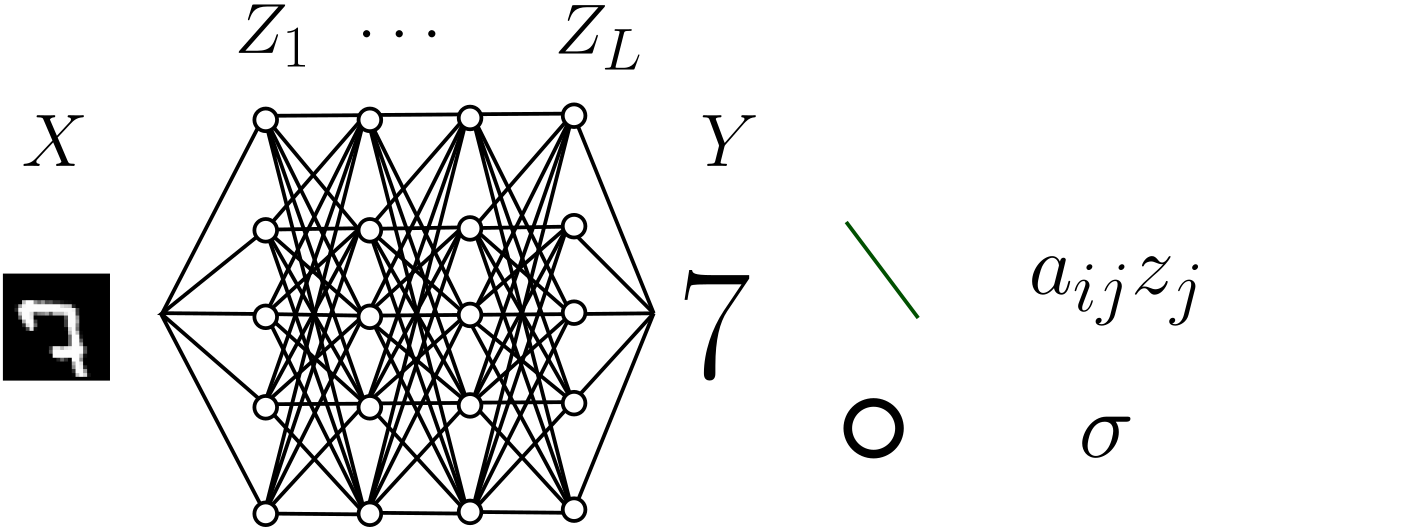
\includegraphics[width=.6\textwidth]{graphics/network_with_expl.png}
    \caption{A neural network. The 'neurons' (components of the vectors in the intermediate spaces) are connected to the next intermediate space by linear connections. Then, a non-linearity is applied (possibly after adding a bias, not shown in the figure).}
    \label{fig:MLP}
\end{figure}



% different non-linearities

% ReLU
% Sigmoid
% softmax
% Multilayered perceptrons

\subsubsection{Why deep neural networks?} The definition of a neural network is not difficult to state, but hard to understand. Why should non-linearities and affine maps be interleaved like this? Why will that lead to well-performing models? To be really honest, there is no really satisfactory answer to this yet -- researchers are still very much debating what the 'true' reason for the success of deep learning. Still, let us give one hand-wavy, and one slightly more mathematical explaination.

\paragraph{A biological motivation} A deep neural network can be viewed as a very simple model of a brain. A brain cell, or neuron, can very naively be thought of as a a cell body to which is attached a couple of \emph{dendrites} and an \emph{axon}. A cell receives stimuli (from some type of chemicals) in the dendrites. If the stimulus exceeds a threshold, it \emph{fires} an electric signal through the axon, and releases neurotransmitters on the other side of the axon, which cause new brain cells to fire. 

This vaguely resembles the functionality of an intermediate function in a neural network: it receives information $\sprod{a^k_i,y}+b^k_i$ (where $y$ is the 'stimuli' from the previous intermediate space), sends it through its non-linearity, and then 'fires' 'stimuli' to the next layer. This explains the terminology 'neurons' for the intermediate functions. See also Figure \ref{fig:neuron}

This mental model should only be understood of as an 'explaination' of the success of neural networks accompanied with a \emph{big} grain of salt. Although it can be a useful food for thought, it ultimately does not explain much.

\begin{figure}
    \centering
    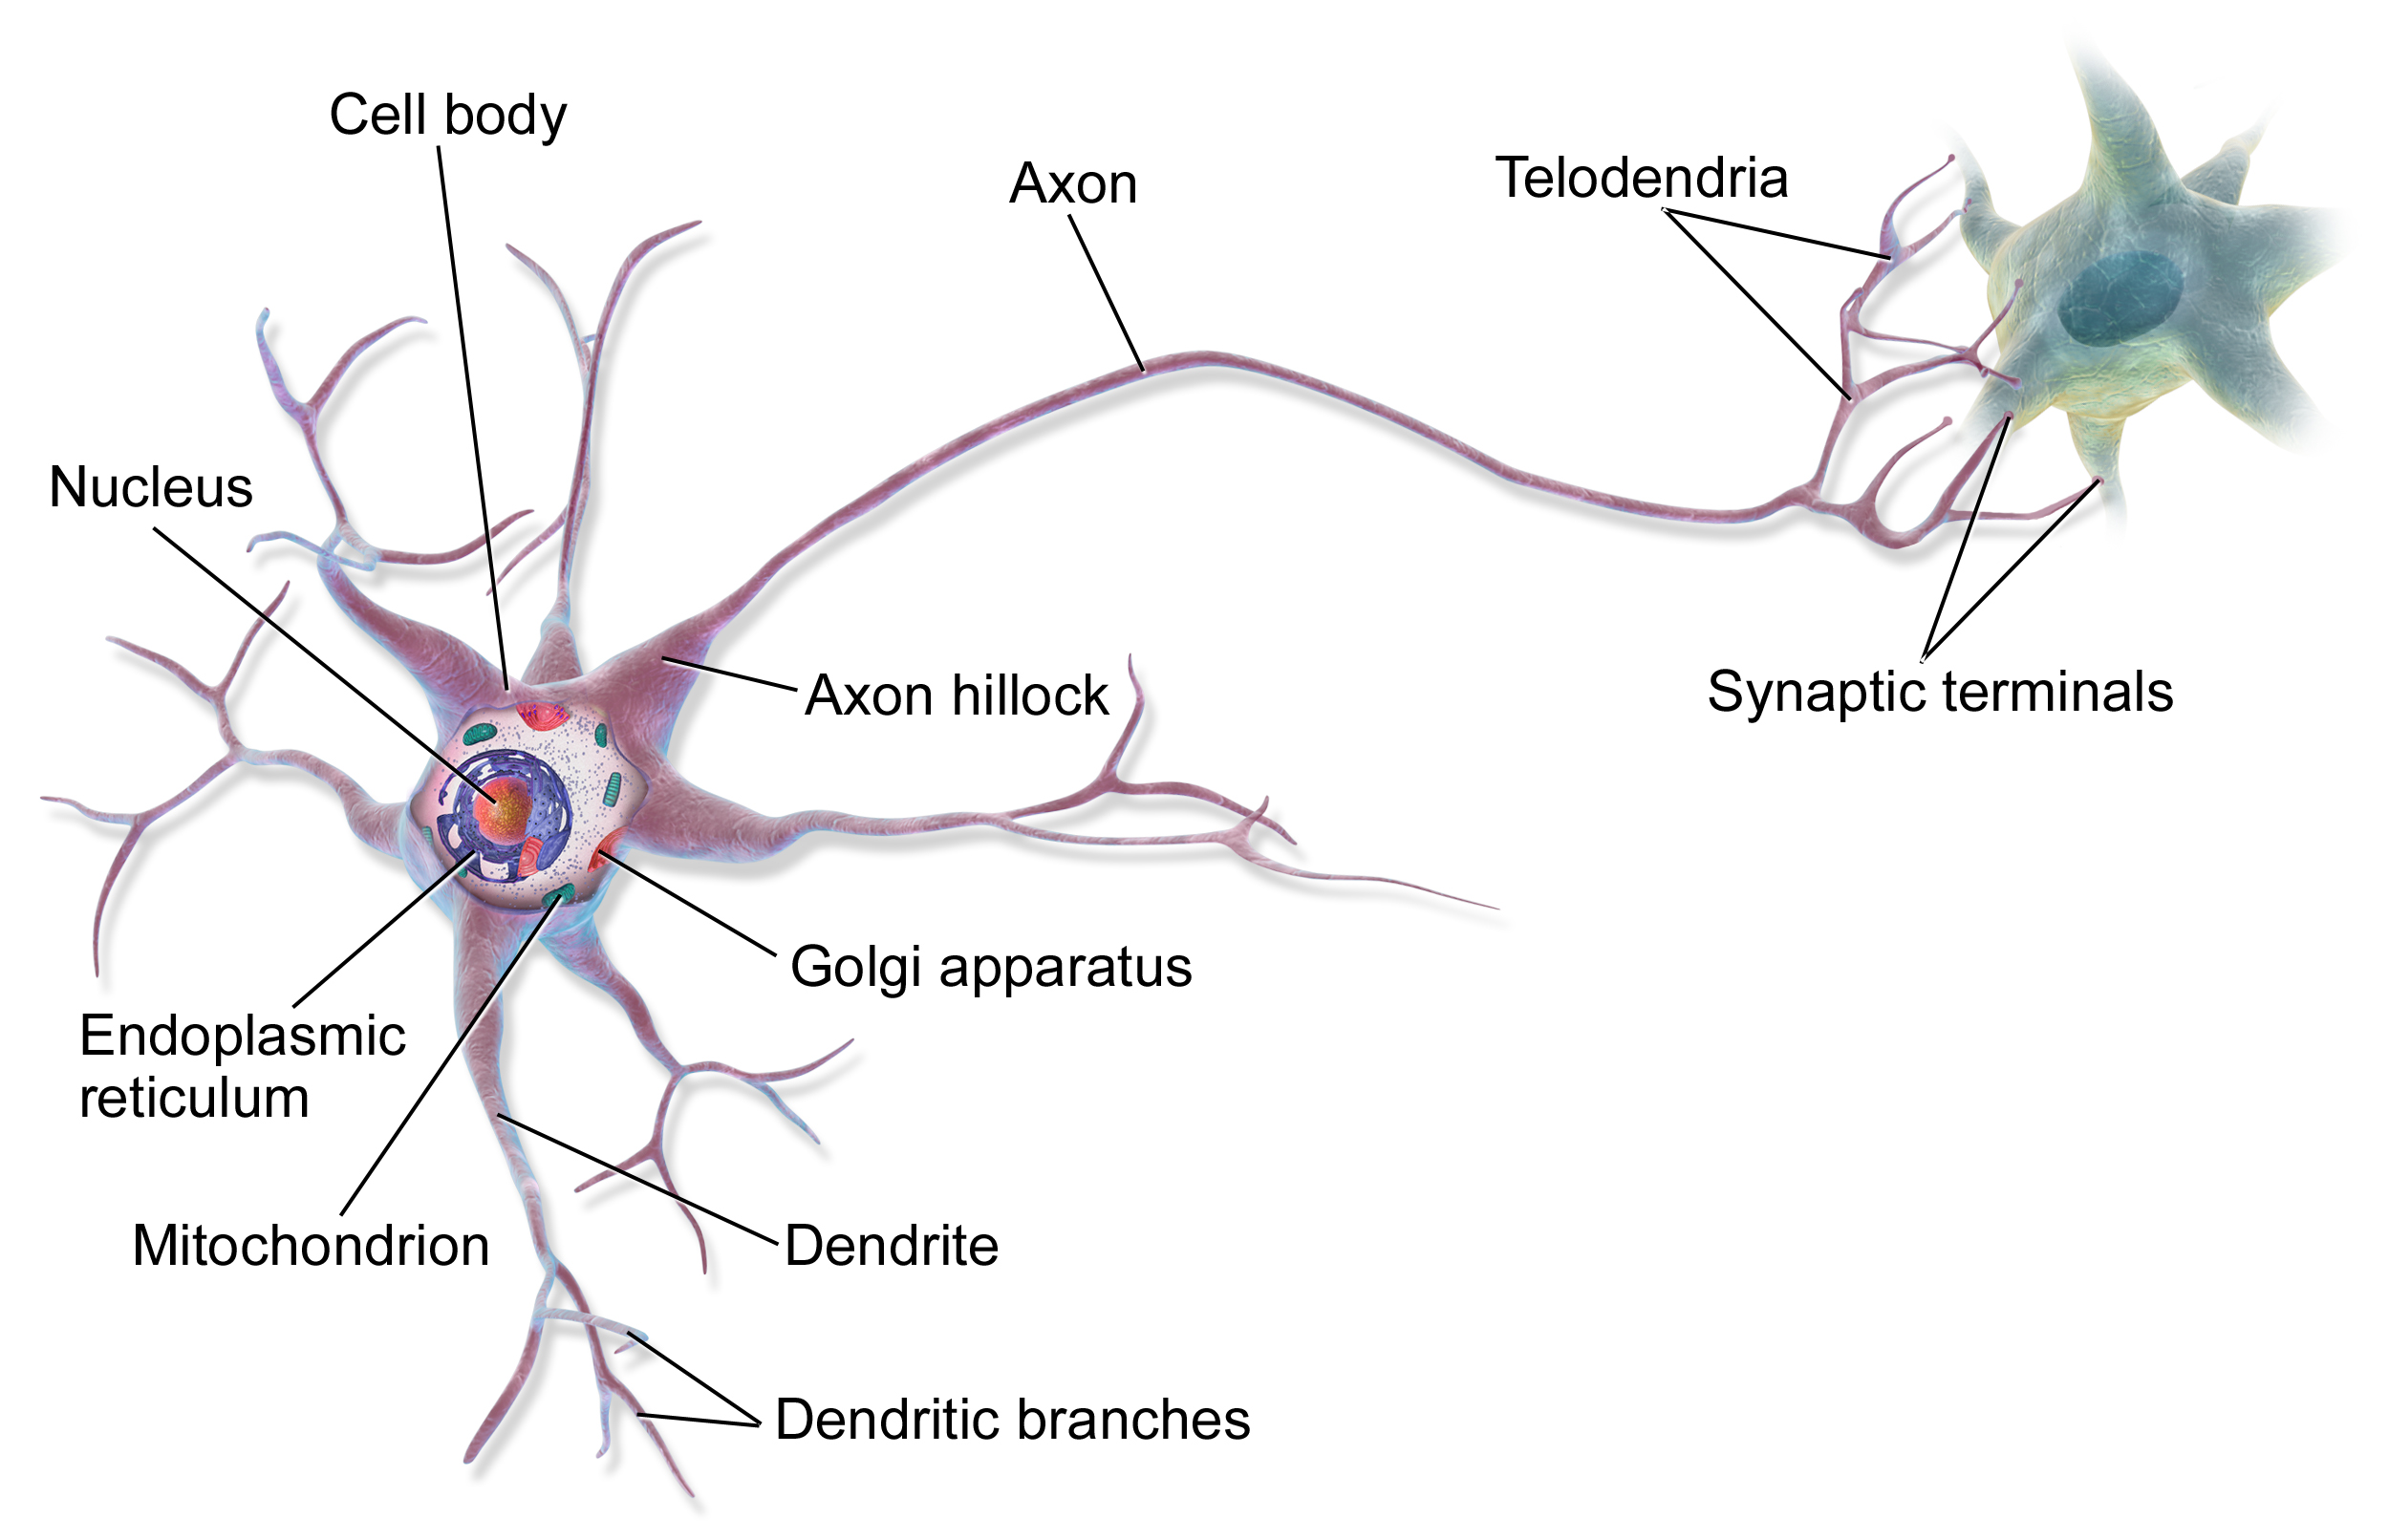
\includegraphics[width=.4\textwidth]{graphics/Blausen_0657_MultipolarNeuron.png}\hspace{.3cm}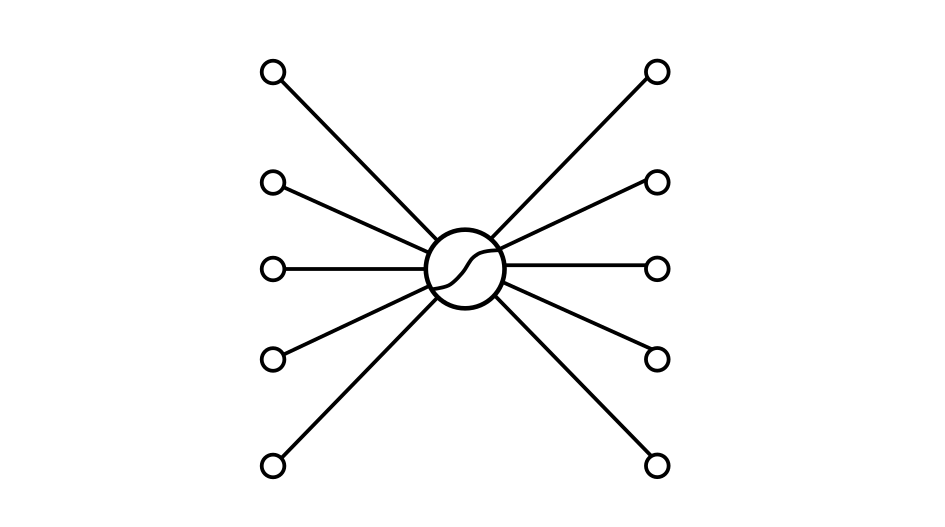
\includegraphics[width=.4\textwidth]{graphics/neuron.png}
    \caption{Left: A biological neuron\protect\footnotemark. Right: A neuron in a neural network.}
    \label{fig:neuron}
\end{figure}

\footnotetext{{By BruceBlaus - Own work, CC BY 3.0, \href{commons.wikimedia.org/w/index.php?curid=28761930}{https://commons.wikimedia.org/w/index.php?curid=28761830}}}

\paragraph{The universality theorem} The \emph{universality theorem} gives a somewhat more mathematical explaination as to why deep neural networks can be applied in such diverse contexts.

\begin{theorem} \label{th:universality} Let $X$ and $Y$ be normed, finite-dimensional vector spaces, and $f: X\to Y$ a continuous function. Furthermore, fix a compact set $C\sse X$, and an activation function $\varsigma$ which is not a polynomial. Then, for any every $\epsilon>0$, there exists a neural network $g: X \to Y$ with $\varsigma$ as its activation function with
\begin{align*}
    \sup_{x\in C} \norm{f(x)-g(x)} <\epsilon.
\end{align*}
That is: The set of neural networks is dense in the set of continuous functions with respect to the topology induced by the supremum norm on compact set.
\end{theorem}

Note that the theorem \emph{does not} say that a fixed architecture is enough to approximate any function. What it rather says is that given a function $f$ there exists \emph{a} network architecture (that can be very 'deep' ($L \to \infty$) and/or very 'broad' ($\dim Z_i \to \infty$)) that can approximate $f$. To get more quantitative bounds ('we can approximate this function using this amount of neurons'), we need to assume additional properties of the function we want to approximate, typically some smoothness.

Hence, although this theorem shows that neural networks potentially can approximate anything, the theorem per se is also of limited practical importance.

We will prove a form of this theorem later. For now, let us continue focusing on practical aspects.



% Quick explaination of the universality theorem

\subsubsection{A few layer types}
Although the definition of neural networks allow for the layers to be any affine-linear function, one often restricts the structure of the layers, to achieve different effects. Let's list a few such choices.

\paragraph{Fully connected layers} The simplest choice is to not restrict the layers at all. This type of layer is commonly referred to as \emph{fully connected}, as there are weights connecting any pair of neurons in the two consecutive intermediate spaces. Architectures with only fully connected layers is sometimes referred to as \emph{multilayered perceptrons}, to distinguish them from other choices.

\paragraph{Convolutional layers} When dealing with images, so-called \emph{convolutional layers} are popular. Here the idea is simply only allow the linear part of the layer to be a \emph{convolutional operator}:
\begin{align*}
    Ax = \phi*x , \quad (\phi*x)(k,\ell) = \sum_{m,n}\phi(m,n)x({k-m,\ell-n}).
\end{align*}
This of course also works with one-, three- and even $n$-dimensional data (although high-dimensional data often is hard to handle practically due to dimensionality reasons). To achieve expressivity (i.e to be able to approximate many functions with the networks), one uses more than one input and more than one output channel (say $M$ and $N$) , so that the actual mapping has the form
\begin{align*}
    \R^{N,n_0 \times n_1} \ni (Ax)_k = \sum_{\ell} \phi_{k,\ell}*x_\ell, \quad x = (x_0, \dots, x_M) \in \R^{M,m_0 \times m_1}.
\end{align*}

\begin{figure}
    \centering
    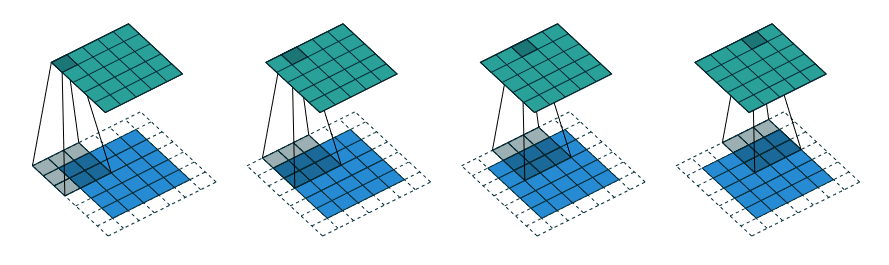
\includegraphics{graphics/convolutional_layer.png}
    \caption{A convolutional operator. From \cite{dumoulin2016guide}.}
    \label{fig:enter-label}
\end{figure}

\begin{figure}
    \centering
    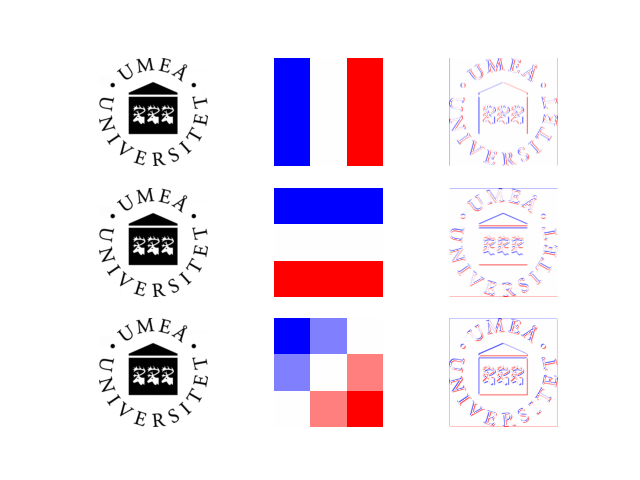
\includegraphics[width=0.75\linewidth]{graphics/filter_fig.png}

    \caption{\label{fig:filter}Images, filters, and results of convolutions. The top filter sense jump-singularities in $x$-direction, the middle one in $y$-direction, and the bottom one in the $(1,1)$-direction. Pay close attention to the effect on the sides of the central square. Best viewed in color.}
\end{figure}

Convolutional layers process similar features in different parts of the data (e.g. images) in the same way. One can imagine that each convolutional map 'senses' if a certain structure is present in an image, and if so, 'tells' us where. To understand what this means, consider the one-dimensional convolutional filter
\begin{align*}
    \phi(k) = \begin{cases}
        1 & \text{ if } k = 0 \\
        -1 & \text{ if } k= 1 \\
        0 & 0 \text{ else}
    \end{cases}.
\end{align*}
Convolving this with a one-dimensional function $x$ yields
\begin{align*}
    (x*\phi)(\ell) = \sum_{k}x(\ell-k)\phi(k) = x(\ell)-x(\ell-1).
\end{align*}
Hence, $(x*\phi)(\ell)$ will only be large if $x$ has a 'jump'  at $\ell$. Hence, $\phi$ 'senses' jump singularities, and where they are. In two dimensions, we can even build filters that sense jump singularities in certain directions -- see Figure \ref{fig:filter}.



Filters used in neural networks are often chosen to have quite small supports -- often only $3\times 3$ or $5 \times 5$ pixels in the image case. This both helps to capture \emph{local information} as well as speed up computations. There are many technical variations of convolutional layers, such as which padding to use, so-called striding, etc. Networks using convolutional layers are often referred to as \emph{CNN}:s, \emph{Convolutional Neural Networks}.





\paragraph{Pooling layers} \emph{Pooling layers} are used to reduce the dimensionality of data. This is both computationally wise and leads to more stable networks -- the effect of changing the position of a feature a pixel or two will diminish a lot. They often have no parameters (and hence to not change during training), but are still handled as layers in implementations.

There are two main strategies for pooling: average- and max-pooling. In both methods, the outputs of groups of neurons (e.g. neighbouring pixels in an image-like feature) are 'squashed together' -- by taking the average, or only keeping the maximum value, respectively.\footnote{Note that max-pooling technically is not a linear map, and hence does not conform to our definition of a layer. However, since these layers are fixed, this will not cause any problems during training.} 



\paragraph{Residual layers} Networks with very many layers (i.e. 'very deep' networks) are often hard to train. To mitigate this, one can use so-called \emph{residual layers}. The idea here is to partially copy the content of the previous output, and only use the layer to adjust it. In more precise terms, one updates between the intermediate features as follows:
\begin{align*}
    x_{i+1} =  x_i + \sigma(A_ix_i + b_i),
\end{align*}
Another alternative is to send the information in (some) neurons further more than one layer forward in the network -- this technique is more generally referred to as \emph{skip connections}. Networks using residual layers are sometimes referred to as \emph{ResNets}. 

An extreme version of ResNets are \emph{Neural ODE}'s. Here, one views the above equation as a discretization of a differential equation:
\begin{align*}    x'(t)=\varphi(x(t)).
\end{align*}
In practice, one then sets up a neural network to approximate $\varphi$, and applies it via solving the above ODE numerically (via for instance some Runge-Kutta method).
\newline 

\begin{figure}
    \centering
    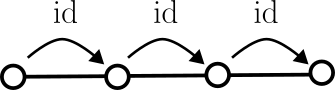
\includegraphics[width=0.45\linewidth]{graphics/resnet.png}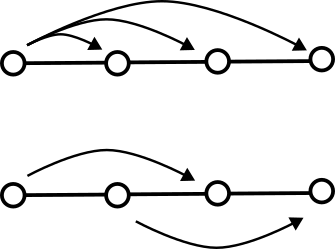
\includegraphics[width=0.45\linewidth]{graphics/skip_connections.png}
    \caption{Left: The structure of a residual net. Right: Two other structures with skip connections.}
    \label{fig:skip_con}
\end{figure}

A neural net seldom only have one type of layer. A very common way to handle image data, for instance, is to first apply convolutional layers, maybe interleaved with pooling layers, to end with one or more fully connected layers to get to the actual output.



% convolutional layers

% pooling

% Outlook: attention


\subsection{Training of deep neural networks}
Once the architecture has been designed, one still needs to \emph{train} the network. Training the network is, again, just another way of saying that we choose the weights and biases of the layers to minimize a risk
\begin{align*}
    R(\theta) = \sum_{i \in [n]} \ell(g_\theta(x_i),y_i) 
\end{align*}
where $g_\theta$ is the deep neural network -- we have here -- to simplify the notation --  abstracted the values of all weights and biases into one object $\theta$. It has turned out that this can be accomplished by astonishingly simple means -- in principle, a simple \emph{gradient descent} suffices:
\begin{align*}
    \theta_{k+1} = \theta_k - \gamma \nabla R(\theta_k)
\end{align*}
The idea of gradient descent is simple -- $-\nabla R(\theta_k)$ is the direction in which the function $R$ descends most steeply. In order to find values where the function is smaller, we should hence move in that direction. $\gamma$ is called the \emph{learning rate}. This is a parameter that needs to be tuned -- if one uses a too big value, the optimization will often fail to find the 'valleys' of the optimization, but if one uses a too small, the optimization will be very slow (and more easily get stuck in bad local minima). 


\paragraph{The remarkable success of gradient descent}
'Simple' theory of gradient descent says that if we assume that $R$ is strongly convex and we use a correctly tuned learning rate, the gradient descent will converge to the global minimum of the function. When $R$ is the risk of a neural network, there are however no reason for $R$ to have that simple form! $R$ can be highly non-convex, and have many local minima. Although the reason why gradient descent works so well for neural networks to some extent remains a mystery, some mathematical theory has recently emerged that provide some explaination why gradient descent still works so well. The buzzword here is \emph{neural tangent theory} \cite{jacot2018neural}, and the gist of the theory is that when the layers of the networks become very very wide, the optimization landscape of $R$ become no more complicated than that of a standard, least squares linear regression. 

Still, optimizing a neural network is tricky in practice, and many tricks have been engineered to help us. Let us take the time to get aquainted with some of them.

\subsubsection{Backpropagation}
Backpropagation is not so much a trick as it is an efficient way to calculate the derivative of the risk with respect to the parameters of the network. Before diving into the formulas, which to be honest are not that nice, let us explain its main importance: The formulas are \emph{recursive} -- the entities needed to calculate the derivative with respect to the $k$:th layer are calculated 'on the fly' during either the application of the network (the 'forward pass') or when the derivative with respect to the $(k+1)$ layer is calculated (the previous step of the 'backward pass'). Layers can also be treated in the same way wherever they are situated in a bigger network, enabling the calculation of the gradients for networks of arbitrarily complicated architectures.



\paragraph{The formulas}  We assume that the non-linearities $\sigma$ are differentiable -- this requires some eye-squinting in certain points for e.g. $\ReLU$, but since the points of non-differentiable of the ReLu are isolated, they will in practice almost never cause any problems. Let us also fix some notation for the 'hidden neuron functions': we iteratively define
\begin{align*}
    z_0(x) = A_0x+ b_0, \quad z_{i}(x) = A_i\sigma(z_{i-1}(x))+ b_i 
\end{align*}
The deep neural network function $g(x)$ is then equal to $z_L(x)$. The chain rule then immediately implies 
\begin{align}
    \nabla_{A_k} R = \sum_{i \in [n]} \left(\frac{\partial z_{L}(x_i)}{\partial A_k}\right)^*\nabla_1\ell(z_L(x_i),y_i),\quad  \nabla_{b_k} R = \sum_{i \in [n]} \left(\frac{\partial z_{L}(x_i)}{\partial b_k}\right)^*\nabla_1\ell(z_L(x_i),y_i). \label{eq:derivative_risk}
\end{align}
We hence need to calculate the partial derivatives of the $z_L(x_i)$ with respect to the $A_k$ and $b_k$. Since $z_L$ depends on the earlier neuron values $z_k$, we again need to apply the chain rule. We arrive at the following recursion formula:
\begin{align*}
 \left(\frac{\partial z_{\ell}(x_i)}{\partial A_k}\right)^* u =  \left(\frac{\partial z_{\ell-1}(x_i)}{\partial A_k}\right)^*\sigma'(z_\ell(x_i))^*A_\ell^*u, &\quad   \left(\frac{\partial z_{\ell}(x_i)}{\partial b_k}\right)^* u=  \left(\frac{\partial z_{\ell-1}(x_i)}{\partial b_k}\right)^*\sigma'(z_\ell(x_i))^*A_\ell^*u ,  &\ell>k \\
    \left(\frac{\partial z_{k}(x_i)}{\partial A_k}\right)^* u = u \sigma(z_{k-1}(x_i))^*, &\quad   \left(\frac{\partial z_{k}(x_i)}{\partial b_k}\right)^* u = u, & \\
    \left(\frac{\partial z_{\ell}(x_i)}{\partial A_k}\right)^* u = 0, &\quad   \left(\frac{\partial z_{k}(x_i)}{\partial b_k}\right)^* u = 0,  &\ell<k
\end{align*}
We see that in order to calculate the derivatives, we need to keep record of the current values of $A_i$ and $b_i$, and 
\begin{itemize}
    \item The 'top' derivatives $\nabla_1\ell(z_L(x_i),y_i)$
    \item The values of the neurons $z_\ell(x_i)$
    \item The values of the 'neuron derivatives' $\sigma'(z_\ell(x_i))$,
\end{itemize}
and that all of them can be calculated through \emph{one} backward pass -- the entities needed to calculate the derivative with respect to the $k$:th layers are calculated while the derivatives with respect to the $(k+1)$:st layer are.
% Explaination of back propagation - one of the reasons training of neural networks is 'simple'


\subsubsection{Stochastic gradient descent}
In the calculation \eqref{eq:derivative_risk}, we need to evaluate the gradient
\begin{align*}
    \nabla_\theta \ell(g_\theta(x_i),y_i)
\end{align*}
for \emph{every} data point $x_i$. Considering the huge amounts of data  ($n\approx 10^4$ is considered small) typically used in application of deep learning, this is not really feasible. Since the calculations are independent of each other, we could perform the calculations in parallel, but that will quickly lead to memory issues.

The solution of these problems is surprisingly simple. Instead of using all data in each step, we only use only one, or a few, examples, take a step, and move on with the next 'mini-batch' of data. In other words, in each step, we calculate the gradient of 
\begin{align*}
    R_0(\theta)= \sum_{i \in I_0} \ell(g_\theta(x_i),y_i)
\end{align*}
for some subset $I_0$, and use it to update our parameters. Once we have looked at all the data (this is referred to as an \emph{epoch}), we can start over. 

This procedure is referred to as a \emph{stochastic} gradient descent (SGD). The line of thought here is that the mini-batch of data we consider is drawn randomly, and that $R_0$ hence is a \emph{stochastic approximation} of the 'actual risk' $R$. This completely corresponds to what happen within each epoch, but we call also the algorithm applied to 'periodically recycled data' SGD. There is a whole theory of such \emph{stochastic optimization}, which we will not delve in deeper here.

\paragraph{Example} Stochastic gradient gives a nice interpretation to \emph{ELO rating systems}. ELO rating systems are used to determine the relative strengths of players two-player games, such as chess (or teams in match-based sports, such as football). Each player is given an initial rating $R$ when they enter the ranking system. When a game is played, the ratings of the competing players is updated, depending on the relative strenghts of the player -- if a clear underdog wins, their rating will rise a lot, but it will not drop much if they lose (since this is the expected result), and vice versa. The formula used is the following:
\begin{align}
    R^{\mathrm{new}} = R^{\mathrm{old}} + K(S_A-E_A) \label{eq:ELO_update}
\end{align}
where $S_A$ is the result in the match ($1$ for a win and zero for a loss) and $E_A$ is the the expected result (probability of a win). 

To explain why this system will lead to good estimates of the strengths of the players, let us think about what the purpose of the rating is -- it is there to estimate the probability of one player winning over the other. The data we have at our disposal to estimate the outcome of a match are the outcomes of the matches we have recorded. We can encode the results as $y_i \in \{-1,1\}$ and the matches $x_i \in \R^p$, where $p$ is the number of players that are participating, and $x_i(k)=1$ if player $k$ was player $A$, and $x_i(k)=-1$ if player $k$ was player $B$. Since the outcome of a match is binary, it is reasonable to use a logistic model:
\begin{align*}
    p_\beta(x) = \varphi(\sprod{\beta,x}) =  \frac{e^{\sprod{\beta,x}}}{1+e^{\sprod{\beta,x}}} = \frac{1}{1+e^{-\sprod{\beta,x}}}
\end{align*}
$p_\beta$ here refers to the probability of player $A$ winning.
The prediction the probability that player $k$ beats player $\ell$ is then
\begin{align*}
    \frac{1}{1+e^{-(\beta_k-\beta_\ell)}}.
\end{align*}
We interpret the $\beta_k$ as the ratings of the players!

To fit the logistic model, we should choose $\beta$ to minimize the $\log$-likelihood
\begin{align*}
    -\sum_{i \in [n]} y_i \log(p_\beta(x_i)) + (1-y_i) \log(1-p_\beta(x_i)).
\end{align*}
Applying a step of stochastic gradient descent with a minibatch of one training example will lead to an update of the vector $\beta$ corresponding to \eqref{eq:ELO_update} (where $y_i=S_A$ and $E_A=p_\beta(x_i)$ for the update of the player $A$ rating). The ELO-rating is hence trying to continuously fit a logistic model through SGD!

\begin{proof}
    Let us say that the match $x_0$ in the minibatch is between player $k$ and $\ell$. We have
    \begin{align*}
        p_\beta(x_0) &= (1+\exp(-\sprod{\beta,x_0})^{-1} = (1+\exp(-(\beta_k-\beta_\ell))^{-1} \\
        1-p_\beta(x_0) &= 1- (1+\exp(-\sprod{\beta,x_0})^{-1} = (1+\exp((\beta_k-\beta_\ell))^{-1}.
    \end{align*}
    Consequently,
    \begin{align*}
        y_0 \log(p_\beta(x_0)) + (1-y_0) \log(p_\beta(x_0)) =\begin{cases}
            - \log(1+\exp(-(\beta_k-\beta_\ell)))  &\text{ if $y_0=1$} \\
            -\log(1+\exp((\beta_k-\beta_\ell)))  &\text{ if $y_0=0$}
        \end{cases} 
    \end{align*}
    Hence, with $R_0 = - y_0 \log(p_\beta(x_0)) - (1-y_0) \log(p_\beta(x_0))$, we get if
    \begin{align*}
        [\nabla R_0](k) = \begin{cases}
            \frac{\exp(-(\beta_k-\beta_\ell))}{ 1+\exp(-(\beta_k-\beta_\ell)))}  &\text{ if $y_0=1$} \\
            -\frac{\exp((\beta_k-\beta_\ell))}{ 1+\exp(-(\beta_k-\beta_\ell)))}  &\text{ if $y_0=0$}
            \end{cases} = \begin{cases}
                1-p_\beta(x_0)  &\text{ if $y_0=1$} \\
            - p_\beta(x_0) &\text{ if $y_0=0$}
            \end{cases} = y_0 - p_\beta(x_0),
    \end{align*}
    and similarly  $[\nabla R_0](\ell) = -(y_0 - p_\beta(x_0))$. All the other components of $\nabla R_0$ are obviously $0$. 
    
    Since $y_0$ is the result of the match, i.e. $S_A$, and $p_\beta(x_0)$ is the prediction, i.e. $p_A$, we have thus shown that an $SGD$ update will add a constant times $S_A-E_A$ to the ratings of the participating players, as claimed.
\end{proof}




We mainly motivated SGD through its computational cheapness, but this is not the only benifit of $SGD$. For example, its stochastic nature will help it 'escape' shallow local minima -- se Figure \ref{fig:sgd}.

\begin{figure}
    \centering
    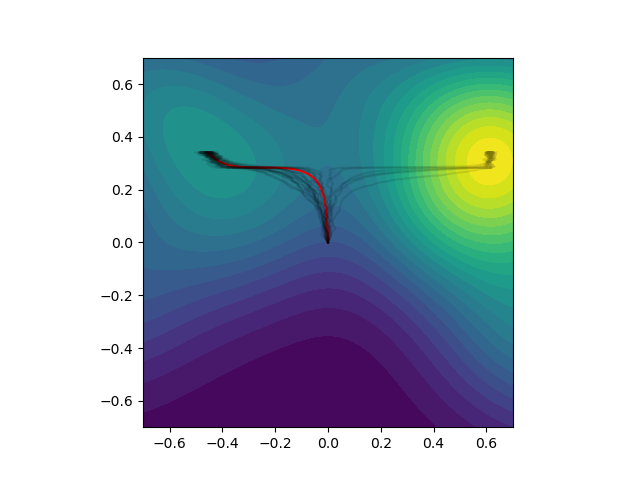
\includegraphics[width=.6\textwidth]{graphics/sgd.png}
    \caption{The trajectory of a gradient descent (red) and the trajectories of stochastic gradient descent (black) for a non-convex function. Notice that many of the runs of SGD follow the gradient descent path, but that some 'escape' the local minimum and find a better point than gradient descent.}
    \label{fig:sgd}
\end{figure}

% Gradient descent vs. stochastic gradient descent

\paragraph{Other learning algorithms}
Stochastic gradient descent is an iconic optimization procedure in deep learning, but often not the most efficient. An important class of algorithms are those that try to, in an automatic fashion, adaptively update the learning rate $\gamma$, to allow for large steps when they can be taken, but to make them smaller as $\theta$ is approaching a local minimum. An important example is the $\mathrm{ADAM}$ algorithm. If the training of a network is slow, it may definitely be a good idea to try one of these more sophisticated algorithms, but we will not attempt to describe them in detail here.

% ADAM et concortes


\subsubsection{Batch normalization} Sometimes, learning can stall simply because the parameters are started in a region of space where gradients are small in norm. Imagine for instance a network with quite large weights using a $\tanh$-nonlinearity. The large weights will cause the neurons to report back large values $z$, so that $\tanh'(z)$ is small. These problems will disappear once the weights (and therefore values of $z$) have shrunk, but this can take a while.

To mitigate such effects, one can use something \emph{batch normalization}. The idea here is that problems like the ones above will be more unlikely if only the values of the features -- \emph{in all layers} --  are properly normalized -- note that by adjusting the values of the final weights, we should still be able to realise the same functions although we perform such a normalization, even in each layer.

In mathematical terms, we would like each layer to operate on, instead of the actual values $z_k(x)$, the normalised values
\begin{align*}
    \tilde{z}_k(x) = \frac{z_k(x) -\mathbb{E}(z_k(x))}{\sqrt{\mathbb{V}(z_k(x))}},
\end{align*}
where the expected value and variance is taken over the available training data. This is referred to as \emph{batch normalization}. One could also imagine shifting the values by a learnable additive and multiplicative factor $\beta$ and $\gamma$, respectively:
\begin{align*}
    \tilde{z}_k(x_i) = \frac{z_k(x_i) -\mathbb{E}(z_k(x))}{\sqrt{\mathbb{V}(z_k(x))}}\cdot \gamma + \beta.
\end{align*}

But how do we calculate the expectation and variance of $z_k$ before we know what $z_k$ should look like? The answer is that we really can't. In practice, this is solved as follows:
\begin{itemize}
    \item During training, keep running estimates $e$ of $\mathbb{E}(z_k(x))$ and $v$ of $\mathbb{V}(z_k(x))$, that are used to normalize each batch of training data.
    \item After training, we fix the estimates and use them during the evaluation of the network.
\end{itemize}


\subsubsection{Dropout} Neural networks with many parameters are flexible, and hence there is a non-zero chance that they overfit, in particular when not fed enough data. A method designed to mitigate overfitting is \emph{dropout}. The dropout method consists of, during training, randomly replacing some of the neuron values with a zero before sending it to the next layer. By doing this, the hope is that smaller 'subnetworks' of the network are trained to perform decently on their own. At inference, we use the entire network, but scale the neurons appropriately.

We can understand dropout in two ways.
\begin{itemize}
    \item An ensemble method -- we combine the 'weak' subnetworks to form a strong entire network. This analogue should be used with caution: differently to the ensemble methods we discussed before, the weak learners are not combined through a linear combination (additive), but rather through a rather convoluted process of 'averaging' in each neuron.
    \item A stochastic optimization method -- in each step, we optimize a different object, which in mean is similar to the object we really want to optimize. This analogue should also be used with caution -- the mean of the subnetworks is actually slightly different to the final network we use, but the difference is relatively small.
\end{itemize}
\paragraph{Remark} Networks can of course also be used in 'true' ensemble learning. This can however be quite expensive, since we need to store and train several neural networks in parallell.

\subsubsection{Data augmentation} Deep networks are known for being 'data hungry' -- they need to look at quite many examples before they 'understand' what is going on. It may therefore be a good idea to artificially create new data examples via taking the data one already has and randomly transforming them. The transformations are typically chosen so that the transformed examples again lead to 'plausible' examples: one can for instance randomly crop, rotate or translate an image, change the colors, masking parts of the image, and so on\footnote{One can also try to do something more wild -- it has (empirically) been shown that augmentation by random Möbius transformation can increase performance on an image classification task \cite{zhou2021data}}. In this way, the networks should also get more stable against such 'impurities' in the test data. See also Figure \ref{fig:augment}.

\begin{figure}
    \centering
    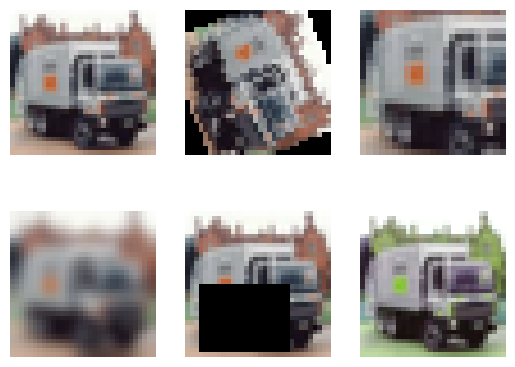
\includegraphics[width=0.65\linewidth]{graphics/augmentation.png}
    \caption{An image from the CIFAR10 dataset (top left), and the result of applying a few data augmentations on it (rotation, cropping, bluring, erazing and color jittering).}
    \label{fig:augment}
\end{figure}

\subsection{Attention}
Let us present one more type of neural network architecture -- \emph{attention layers}. Attention layers are the workhorses of \emph{transformer architectures} \cite{vaswani2017attention}], that have revolutionized the use of neural networks in \emph{natural language processing}. They are for instance key components in the ChatGPT model. Let us give a very brief intro here just to make ourselves acquainted with the concept -- so that we easier can learn more about the details when we are faced with implementing one for real.

To motivate the use of attention, let us first discuss some general concepts of natural language processing. The input data is a \emph{sequence of words}. Each word is assigned a vector (called \emph{token}) in some space $\R^p$ (this is referred to as \emph{embedding} the sequence into \emph{feature space}). The output depends on the data -- let us for know consider the task of document classification, where the output is a binary variable (which for instance can represent whether a review is positive or not). Our task is to map a sequence $x(0), \dots, x(L)$ of vectors to a binary variable $y$. In language, word order is crucial ("Statistical learning is interesting" means something completely different to "Interesting learning is statistical"). Therefore, we should try to take the sequential nature of the data into account!

A first idea for handling sequential data is \emph{Recurrent Neural Networks}, RNNs. Here, we let the vector handle a state vector $\eta \in \R^d$ that we sequentially update with the help of the input tokens. After the final update, we extract information from the state vector. Mathematically, this looks like this in its most basic form:
\begin{align*}
    \eta(k) = \sigma(U\eta(k-1) + Wx(k-1)), \quad y = B\eta(L)
\end{align*}
Here, $U,W$ and $B$ are the weights of the network. Importantly, they are the same for each $k$. One can also use nonlinear maps instead, but this approach will have a fundamental problem: \emph{long term dependence}. We can roughly explain this through the following theorem:
\begin{lemma}
    Let $\sigma$ be the identity. Then, for almost all $U$ with $\ell_2$-operator norm less than or equal to $1$, there exists a vector $w\in \R^p$ with the following property: Let $x$ and $x'$ be sequences that only differ in the first token, and $y, y'$ the corresponding $k$:th outputs. Then
    \begin{align*}
        \lim_{k\to \infty} \norm{y - y'}_2 \leq \abs{\sprod{w,x-x'}}.
    \end{align*}
\end{lemma}
\paragraph{Remark:} The assumption that $\norm{U}_{2\to 2}\leq 1$ is reasonable -- if we do not assume that, the norm of the $\eta(k)$ will explode. 
\begin{proof}
    When $\sigma=\id$, it is not hard to show that
    \begin{align*}
        \eta(k) = U\eta(k-1) + Wx(k-1) = U^2\eta(k-2) + UWx(k-1) + Wx(k) = \dots = \sum_{\ell=0}^k U^{k-\ell}Wx(\ell).
    \end{align*}
    Since $x$ and $x'$ only differ in the first token, we get
    \begin{align*}
        y-y'- = B\eta(k)-B\eta(k)' = BU^kx(0) - BU^kx(0)'.
    \end{align*}
    Now consider an eigenvalue value decomposition of $U$: $U = \sum_{i \in [r]} \sigma_i w_iw_i^* \implies U^k = \sum_{i \in [r]} \sigma_i w_iw_i^*$. For almost all $U$, all but one eigenvalue is strictly smaller than $1$. Consequently,
    \begin{align*}
        \lim_{k \to \infty } \norm{BU^kx(0) - BU^kx(0)'} \leq  \norm{Bw_0w_0^*(x(0)-x(0)')}_2 = \abs{\sprod{\norm{Bw_0}w_0,x(0)-x(0)'}},
    \end{align*}
    which is the claim.
\end{proof}
What the above means is that almost always, no matter the dimensions of RNN network and structure of the weights, the output will essentially only depend one of the maybe hundred dimensions in the first token $x(0)$. Hence, it is 'washed out'. There are ways to mitigate this that keeps the 'modify an evolving state-vector'-idea. Skip connections is one idea, another one is to make the modification mechanism more complicated -- this leads to so called LSTM (\emph{Long and Short Term Memory}) networks. 





\paragraph{Attention} A more radical way of handling the problem is given by \emph{attention layers}\footnote{What we are describing here is \emph{dot-product self attention}. There is a myriad of other variants of attention in the literature, but they all build on the same ideas}. Here, we let each token in the sequence \emph{attend} to all other tokens in the sequence, and depending on which other tokens are present in the sequence, change the output $y$ in different ways. Mathematically, this can be done as follows. First, each token in the sentence are mapped to \emph{key}, \emph{query}  and \emph{value} vectors through learnable weight maps:
\begin{align*}
    q(i) = Qx(i), k(i) = Kx(i), v(i) = Vx(i)
\end{align*}
Then, the keys and queries are checked for 'connectedness' by computing inner products $\omega_{ij} = \sprod{k_i,q_j}$. For each key, we then apply a softmax function over the key-dimension to obtain \emph{attention weights}
\begin{align*}
    \alpha_{ij} = \softmax_{j'} \omega_{ij'}.
\end{align*}
Then, we take a weighted sum over the values to obtain a 'total value' of the query i
\begin{align*}
    y_i  = \sum_{j} \alpha_{ij} v(j)
\end{align*}
The sequence of vectors $y_i$ can thereafter be processed, for instance through a fully connected neural network layer, to produce the input.
In this manner, the impact of the words on the output can change \emph{depending on the context} of the other words: for instance, the word 'waste' can be handled differently in the two sentences 'It was a waste of time to watch this' and 'It is a waste that not more people have seen this'. In the first case, 'waste' can cause the output to drift towards 'bad review', whereas in the second, it can cause it to move towards 'good review'. And crucially, it can do so even if it is on in the very beginning of the sentence!

\paragraph{Remark} It should be noted that when we compare keys and queries like above, the order of the word in the sentence will not matter at all. This can be mitigated by the use of a \emph{positional embedding} map, which encodes the index $k$ of a word into a vector $w$. \newline




\subsection{Proof of universality of ReLU-networks} Let us end the section on neural networks by proving a version of the universality theorem. The theorem has many proofs. The 'standard' one for the most general setting uses quite advanced tools from functional analysis \cite{hornik1989multilayer}, and we will therefore not present it here. We will here present a simpler, but also more illustrative, proof for the case of $\varsigma$ being the ReLU. We will furthermore also assume that $X=Y=\R$, and $C=I$ is a compact interval.

\begin{proof}[Proof of Theorem \ref{th:universality} for ReLU networks.]
    In fact, two-layer neural networks be enough. Let us define $\calN$ as the set of such networks, i.e.
    \begin{align*}
        \calN = \{\sum_{\ell \in [k_1]} a_\ell^1\varsigma(a_\ell^0 x + b_\ell^0) + b^1 \, \vert \, k_1 \in \N, a_\ell^1, a_\ell^0, b_\ell^0 \in \R, \ell \in [k_1], b^1 \in \R\}.
    \end{align*}
    In words, $\calN$ is equal to the set of linear combinations of (span of) functions of the type $\varsigma(a_\ell^0 x + b_\ell^0)$. We will in the following 'build' more and more complicated functions by constructing such linear combinations. Note that we always can use linear combinations of the 'building blocks' we have already constructed and not leave the span. 

    \paragraph{Step 1: A 'hat' ReLu- NN} Let $x_0<x_1<x_2 \in I$ be arbitrary and consider the 'hat function'
    \begin{align*}
        \phi_{x_0,x_1,x_2}(x) = \begin{cases}
            0 & \text{if } t<x_0 \\
            \tfrac{t-x_0}{x_1-x_0} &\text{if } x_0 \leq x <x_1 \\ 
             1-\tfrac{t-x_1}{x_2-x_1} &\text{if } x_1 \leq x <x_2 \\ 
            0 & \text{if} t\geq x_2
        \end{cases},
    \end{align*}
    that is, the piecewise linear function which is zero before $x_0$, $1$ in $x_1$, and zero after $x_2$. We claim that $\phi_{x_0,x_1,x_2} \in \calN$. We have
    \begin{align*}
        \varsigma(x-x_0) - \varsigma(x-x_1) &= \begin{cases}
            0 & \text{if } t<x_0 \\
            t-x_0 &\text{if } x_0 \leq x <x_1 \\ 
             x_1 - x_0 &\text{if } x_1 \leq x
        \end{cases}
    \end{align*}
    Hence, through scaling the above difference, we build a piecewise linear functions that is equal to $0$ before $x_0$, and equal to $1$ after $x_1$. In the same way, we build one that is $0$ before $x_1$ and equal to $1$ after $x_2$. By taking the difference of those, we obtain one that is $0$ before $x_0$, $1$ in $x_1$ and $0$ after $x_2$ -- i.e. $\phi_{x_0,x_1,x_2} \in \calN$.

     \paragraph{Step 2: Linear combinations of 'hats'} Now take $x_0<x_1<x_2 < \dots < x_n$ and $\omega_0, \dots \omega_n \in \R$ arbitrary. Then
     \begin{align*}
         \sum_{i=1}^{n-1} \omega_i \phi_{x_{i-1},x_{i},x_{i+1}} 
     \end{align*}
     i.e. the piecewise linear functions with 'junctions in the $x_i$, values $0$ in $x_0$ and $x_n$, and $\omega_i$ in $x_i$ is in $\calN$. By also adding a constant and a multiple of $\varsigma(x-x_0) - \varsigma(x-x_n)$, we see that we can write \emph{any} piecewise linear function as a neural network.

     \paragraph{Step 3: Approximation of continuous functions} It is now only left to, for a given continuous functions $f:I \to \R$ and $\epsilon>0$, a piecewise linear function $g$ with $\norm{f-g}_\infty \leq \epsilon$. This is however simple -- since $I$ is compact, $f$ is equicontinuous so that there exists a $\delta$ with $\abs{f(x)-f(y)}< \tfrac{\epsilon}{2}$ for $x-y<\delta$. Now choose a set of junctions $x_i$ with separation $\delta$ in $I$ and let $g$ be the piecewise linear function with those junctions and $f(x_i)=g(x_i)$ for all $i$. For $x$ in any interval $(x_i,x_{i+1})$, we can now argue
     \begin{align*}
         \abs{f(x)-g(x)} &\leq \abs{f(x)-f(x_i)} + \abs{f(x_i)-g(x_i)} + \abs{g(x)-g(x_i)} < \tfrac{\epsilon}{2} + 0 + \abs{g(x_{i+1})-g(x_i)} \\
         &= \tfrac{\epsilon}{2} + \abs{f(x_{i+1})-f(x_i)} < \tfrac{\epsilon}{2} + \tfrac{\epsilon}{2},
     \end{align*}
     which was the claim.
\end{proof}

\subsection{Recommended further reading and exercises} Deep neural networks are treated in Chapter 10 of \cite{james2023introduction}. Good exercises are 10.10.1 and 10.10.4. Consider also the following exercises.

\begin{exercise}
    Argue that a one-dimensional filter of the form $w = [1,-2,1]$ can detect points where the derivative of a continuous function is not continuous.
\end{exercise}

\begin{exercise}
    This is an exercise to get a better intuition of stochastical gradient descent.

    Consider the random function of the form $f(x) = \tfrac{1}{2} x^2 + \lambda x$, where $\lambda$ is a uniformly distributed variable in $[-\alpha,\alpha]$ for some $\alpha>0$. Notice that this function in expectation is equal to $\tfrac{1}{2}x^2$, which has a minimum in $x=0$
    
    (a) Argue that applying stochastic gradient descent to $f(x)$ amounts to iterative updates to a optimization variable $x_k$ of the form
    \begin{align*}
        x_{k+1} = x_k - \gamma(x_k + \lambda_k),
    \end{align*}
    where $\lambda_k$ are random variables uniformly distributed in $[-\alpha,\alpha]$, independent of $x_k$.

    (b) Argue that the expected value of $x_{k}$ obeys $\abs{\mathbb{E}(x_k)} \leq (1-\gamma)^k \abs{\erw{x_0}}$, and hence that this expected value converges to $0$ if $0<\gamma<2$.

    (c) Argue that the variance of $x_k$ obeys $\mathbb{V}(x_k) = (1-\gamma)^2 \mathbb{V}(x_{k-1}) +\gamma^2 \alpha^2/3 $, and from that that $\lim_{k \to \infty}\mathbb{V}(x_k) = \gamma\alpha^2/(3(2-\gamma))$, if $0<\gamma<2$. 

    (d) Can $\gamma$ be chosen so that the $x_k$ converge to $0$ with probability one (i.e., almost surely)? Explain.
\end{exercise}

\begin{exercise}
    Will the universal approximation theorem hold for any activation function? \emph{Tip:} What type of function can a neural network whose activation function is a polynomial represent?
\end{exercise}

\begin{exercise}
    The basic Datatype in the \texttt{PyTorch} package (with which one can train neural networks) is a \texttt{tensor}. The tensor stores two arrays of numbers, the \texttt{data} and \texttt{grad}. Try to explain how these are used when training networks.
\end{exercise}

\section{Sparse linear regression}

In this chapter, we will return to the problem of linear regression in high dimensions. We recall the notation: we assume that the features $y_i$ depend on the features $x$ as $y_i = \sprod{\beta_*,x_i} +\eta_i$ for some \textbf{ground truth} $\beta_*$ and (Gaussian) noise $\eta$. We remember the fundamental problem of linear regression in high dimensions -- when the number of observations $n$ is less than the number of features $p$, there will always be an infinite number of $\beta$ that perfectly explain the data: $Y=X\beta$ will have many solutions.

In Chapter $2$, we acquainted ourselves with the \emph{sparsity} assumption: That is, that the ground truth $\beta_*$ only has a few non-zero coefficents. This assumption is intuitively reasonable: Out of the many possible features, there exists only a few that has a true influence on $y$. If we can find such a $\beta_*$, it will also help us immensely when interpreting the result.

To simplify our discussion later, let us introduce the notion of the \emph{support} of a signal.
\begin{defi}
    Let $\beta \in \R^p$. The support of $\beta$ is the set of non-zero coefficients in $\beta$:
    \begin{align*}
        \mathrm{supp}(\beta) = \{\beta(i) \, \vert \, \beta(i)\neq 0 \}.
    \end{align*}
    We say that $\beta$ is \emph{$s$-sparse} if $\abs{\mathrm{supp}(\beta)}\leq s$.
\end{defi}

In this entire section, we will assume that the ground truth $\beta_*$ is sparse, but we will \textbf{not} assume that we know $\mathrm{supp}(\beta)$. To solve the sparse regression problem in fact boils down to finding $S=\mathrm{supp}(\beta_*)$ -- once we have it, the regression problem can be restricted to that set:
\begin{align*}
    \min_{\mathrm{supp}(\beta)\sse S} \norm{X\beta-Y}_2^2.
\end{align*}
If $s=\abs{S}\leq n$, this is again a simple, 'low-dimensional' linear regression!

\begin{figure}
    \centering
    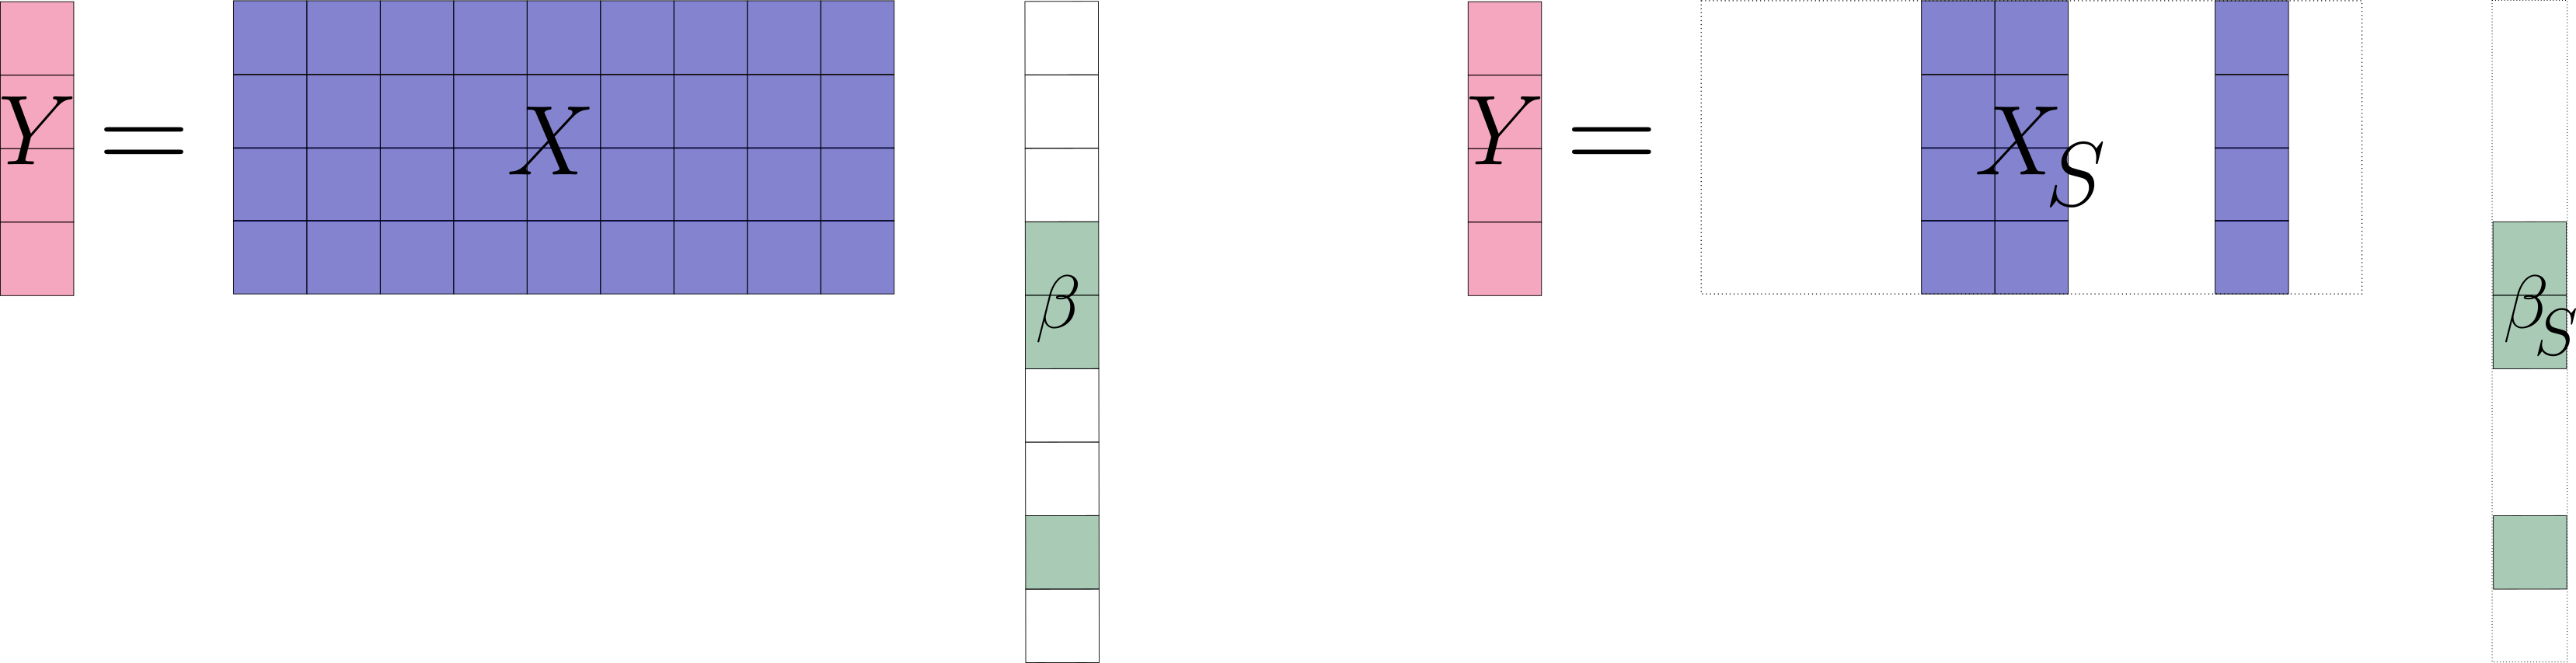
\includegraphics[width=0.85\linewidth]{graphics/sparse_regression.png}
    \caption{Sparse linear regression. $Y=X\beta$ is a priori a problem without a unique solutions, but once $S=\mathrm{supp}\, \beta$ is known, we can reduce to $Y=X_S\beta_S$, which is simple, 'low-dimensional' problem with a unique solution.}
    \label{fig:linreg}
\end{figure}




\subsection{A better greedy method: Orthogonal Matching Pursuit}
In Chapter $2$, we discussed a very simple \emph{greedy} method to solve the sparse regression problem: See which $1$-sparse support (i.e., which feature) can best explain the data on its own, keep that, and then iteratively add new features by checking which new subsets performs the best.

This method works, but it is relatively expensive -- to find an $s$-sparse vector, we will during its course have to solve $p+(p-1)+\dots + (p-s+1) \sim ps$ linear regression problems. This can be improved a lot. We will here discuss a method that only requires $s$ linear regression problems to be solved: \emph{Orthogonal Matching Pursuit} (OMP). It is needless to say that only needing to solve $s$ problems instead of $ps$ is a \emph{huge} improvement in the high-dimensional regime.


OMP is presented in Algorithm \ref{alg:OMP}. Just as forward selection, method iteratively builds estimates $S_0,S_1,S_2, \dots S_k$ of $\mathrm{supp}(\beta_*)$ and approximations $\beta_k$ of $\beta_*$ (where $\mathrm{supp} \beta_k = S_k$. After initializing $S_0=\emptyset$, the idea is to add to $S_k$ the index  $\ell$ that \textbf{maximizes the correlation} between the \textbf{residual} $r_k=Y-X\beta_k$ ('the portion of output left to explain') and \textbf{feature} $\ell$. Assuming the features are all centered and normalized, this can be expressed mathematically as maximizing the scalar product $\abs{\sprod{r_k,X^\ell}}$, where $X^\ell$ is the $\ell$:th column of the data matrix $X$. Note that checking for which $\ell$ the scalar product is largest is very cheap!

One thereafter determines $\beta_{k+1}$ by solving the linear regression problem on the support approximand $S_{k+1}$. It is clear that if we perform $s$ iterations of $OMP$, only $s$ linear regressions need to be solved, which is \emph{much} less than $s\cdot p$, especially in high dimensions ($p\gg 1$). For pseudo-code, see \ref{alg:OMP}.


\begin{algorithm}[tb]      
	\caption{(OMP)} 
	\label{alg:OMP}
	\begin{algorithmic} [1]
 		\REQUIRE Data matrix $X$,  output variables
 		\STATE $S_0=\emptyset$, $r_0 = Y$
 		\REPEAT
 			\STATE Determine the index $\ell$ that maximizes $\abs{\sprod{r_k, X^\ell}}$.
            \STATE $S_{k+1} = S_k \cup \set{\ell}$
            \STATE Determine the solution $\beta_{k+1}$ of 
            \begin{align}
                \min_{\supp \beta \sse S_{k+1}} \norm{X\beta - Y}_2^2 \label{eq:ompprob}
            \end{align}
            \STATE $r_{k+1} = Y-X\beta_{k+1}$
 		\UNTIL stopping criterion is met at $k= k_*$
 		\RETURN $\beta_{k_*}$
	\end{algorithmic}
\end{algorithm}


\paragraph{Analysis of OMP}
As with any other greedy method, there is in general no guarantee that we will find the best sets of $s$ explaining features through OMP. Empirically, it often does quite well though. Can we theoretically explain this? Or put in another way, can we give \emph{conditions} on the data matrix $X$ which \emph{guarantee} that OMP works? This would also give useful information about when OMP is reasonable to apply.

The answer is that we can. The most fundamental and well-known recovery guarantee for OMP is based on \emph{mutual coherehce.}
\begin{theorem} \label{th:OMP}
    Assume that the data matrix $X$ has normalized columns: $\norm{X^i}_2=1$, $i\in [p]$, and define the \emph{mutual coherence} parameter
    \begin{align*}
        \mu(X) = \sup_{i \neq j } \abs{\sprod{X^i,X^j}}.
    \end{align*}
    Also assume that there exists an $s$-sparse vector $\beta_*$ that explains the output, i.e. so that $Y=X\beta_*$. Then, if $$\mu < \frac{1}{2s-1},$$ OMP will output $\beta_*$ after $s$ steps. 
\end{theorem}
\paragraph{Intuition:} Remember that we add variables by checking which feature correlates highly with the residual. If all features are (empirically) weakly correlated, a feature not present in $\mathrm{supp}(\beta_*)$ will not be correlated to $r_0=Y$, and hence not chosen. When we calculate $\beta_1$, we then 'remove' the portion of $Y$ that can be explained by the feature $i_1$, and what is left $r_1$ should then be explainable with the remaning variables. The features not present in $\mathrm{supp}(\beta_*)$ will again give a small correlation value, and we again choose a correct variable, and so on and so forth. In each of the $s$ first steps, we hence pick a new feature, and this feature is one that is present in the ground truth support, so we will be done after $s$ steps.


To give a formal proof of Theorem \ref{th:OMP}, we need the following lemma.
\begin{lemma}
    If $\mu \leq \tfrac{1}{2s-1}$, every submatrix $X_S$ formed by taking columns of an $s$-sparse subset $S$ will be injective.
\end{lemma}
\begin{proof}
    It is enough to prove that $M=X_S^*X_S$ has no zero-eigenvalues (note that this matrix is symmetric, so it is diagonalizable). Let $\lambda$ be an eigenvalue, $v$ an eigenvector, and $k$ the index so that $\abs{v_k}$ is the biggest. We then have
    \begin{align*}
        \abs{\lambda v_k} = \abs{(Mv)_k} \geq \abs{M_{kk} v_k} - \sum_{k \neq j \in S}\abs{M_{kj}v_j}.
    \end{align*}
    Now, $M_{kk}=\sprod{X^k,X^k}=1$, and $\abs{M_{kj}}\leq \mu$ for all $j \neq k$. Since per definition also $\abs{v_j} \leq \abs{v_k}$ for $j\neq k$, we can thus estimate
    \begin{align*}
        \abs{M_{kk} v_k} - \sum_{k \neq j \in S}\abs{M_{kj}v_j} \geq \abs{v_k}(1-(s-1)\mu).
    \end{align*}
    Consequently, $\abs{\lambda} \geq 1 - (s-1)\mu \geq 1- \tfrac{s-1}{2s-1}>0$.
\end{proof}

We can now prove Theorem \ref{th:OMP}
\begin{proof}[Proof of Theorem \ref{th:OMP}]
    Let $S = \supp\beta_*$. We will via induction prove that for all $k\leq s$
    \begin{enumerate}[(i)]
        \item $S_k \sse S$, $\abs{S_k}=k$
        \item There exists a $\gamma_k$ supported on $S$ so that $r_k= X\gamma_k$
        \item $\sprod{r_k,X^\ell}=0$ for all $\ell \in S_k$
    \end{enumerate}
    The case $k=0$ is trivial, since $S_0 = \emptyset$, and that $r_0 = Y = X\beta_*$ per assumption.


    Now let us perform the induction step. Let $\ell$ be the index of the biggest element of $\gamma_k$. Let us bound $\abs{\sprod{r_k,X^\ell}}$ from below:
    \begin{align*}
        \abs{\sprod{r_k,X^\ell}} = \abs{\sum_{j \in S}\gamma_k(j)\sprod{X^j,X^\ell}} \geq \abs{\gamma_k(\ell)}\sprod{X^\ell,X^\ell} - \sum_{\ell \neq j \in S }\abs{\gamma_k(\ell)}\abs{\sprod{X^j,X^\ell}} \geq \abs{\gamma_k(\ell)} (1 - (s-1)\mu).
    \end{align*}
Note that we used that $\ell\in S$, per induction assumption. We also used the definition of $\mu$, the maximality of $\abs{\gamma_k(\ell)}$, and the fact that $\abs{S}\leq 1$.

Now let $i \notin S$. Then $\abs{\sprod{X^j,X^i}}\leq \mu$ for all $j\in S$, and we can bound
\begin{align*}
       \abs{\sprod{r_k,X^i}} = \abs{\sum_{j \in S}\abs{\gamma_k(j)}\sprod{X^j,X^i}} \geq \abs{\gamma_k(\ell)}\mu s.
\end{align*}
This is smaller than $\abs{\gamma_\ell}(1 - (s-1)\mu)$ due to our assumption. Hence, all $\abs{\sprod{r_k,X^i}}$ is smaller than $\abs{\sprod{r_k,X^\ell}}$, and $i$ cannot be chosen in the support extension step. This proves that also $S_{k+1} \sse S$. Also note that due to induction assumption (iii), an index in $S_k$ cannot be chosen again, and hence, $\abs{S_{k+1}}= \abs{S_k} +1 = k+1$.

The next approximation $\beta_{k+1}$ is given by the solution to \eqref{eq:ompprob}, which we know is characterized by the system of equations
\begin{align*}
    X_{S_{k+1}}^*X_{S_{k+1}}\beta_{k+1} = X_{S_k}^*Y  \, \Rightarrow \, X_{S_{k+1}}^*(Y-X_{S_{k+1}}\beta_{k+1}) = X_{S_{k+1}}^*r_{k+1} = 0
\end{align*}
This is just another way to write that $\sprod{X^i,r_{k+1}}=0$ for all $i \in S_{k+1}$, i.e. (iii). It is now only left to note that $r_k = X\beta - X\beta_{k+1} = X(\beta-\beta_{k+1})$, and $\gamma_{k+1}=\beta-\beta_{k+1}$ is supported on $S$.

If we now evaluate what we have proven for $k=s$, we see that $S_s$ is a set contained in $S$ with $s$ indices, i.e. is equal to $S$. Since $\beta_*$ clearly is a solution to 
\begin{align*}
    \min_{\supp \beta \sse S} \norm{X_{S}\beta - Y}_2^2,
\end{align*}
injectivity of $A_S$ then immediately proves that $\beta_s=\beta_*$.
\end{proof}

\paragraph{Remark}
\begin{itemize}
     \item There are many other iterative algorithms to solve sparse regression. Two are called are CoSamp \cite{needell2010cosamp} and HTP \cite{foucart2011hard}.
    \item The stopping criterion is a matter of fine-tuning. One can for instance stop iterating when $\norm{r_k}$ falls below some tolerance level, or when $\abs{S_k}$ reaches a certain size. In practice, this tolerance-level/size should be tuned, using for instance cross-validation.
\end{itemize}


\paragraph{When is $\mu(X)$ small enough?} As we mentioned, the mutual coherence is a measure of the \emph{empirical} pairwise correlations of the features in the random data vector $x$. Remember that we have assumed that the data matrix has normalized columns --  this is not a problem in practice, since we always can achieve that through preprocessing. To check whether OMP works, we are hence actually interested in the behaviour of
\begin{align*}
    \sup_{i \neq j}  \frac{\abs{\sprod{X^i,X^j}}}{\sprod{X^i,X^i}^{\sfrac{1}{2}}\sprod{X^j,X^j}^{\sfrac{1}{2}}}
\end{align*}
Let us write out the scalar product $\sprod{X^i,X^j}$;
\begin{align*}
    \sprod{X^i,X^j} = \sum_{k \in [n]} x_k(i)x_k(j).
\end{align*}
Note that we are here summing over the sample dimension. The above is hence a sum of i.i.d copies of random variables.
Such sums obey the central limit theorem. If we assume that 
\begin{itemize}
    \item The features are uncorrelated, i.e. $\mathbb{E}(x(i)x(j))=0$
    \item The features have unit variance, i.e. $\mathbb{E}(x(i)^2)=1$
\end{itemize}
the central limit theorem implies that for high values of $n$,
\begin{align*}
    \frac{1}{\sqrt{n}} \left(\sum_{k \in [n]}\left(x_k(i)x_k(j)\right) \sim \mathcal{N}(0,\mathbb{E}(x(i)^2x(j)^2)\right), i \neq j \\
    \frac{1}{\sqrt{n}} \left(\sum_{k \in [n]}\left(x_k(i)^2- 1\right) \sim \mathcal{N}(0,\mathbb{E}(x(i)^4)\right),
\end{align*}
Assuming that $\mathbb{E}(x(i)^2x(j)^2)\leq K$ for some common $K$, we can thus argue with high probability that
\begin{align}
    \abs{\sprod{X^i,X^j}} \leq C \sqrt{n}, \quad \norm{X^i}_2^2 = n \pm C\sqrt{n}
\end{align}
for some constant $C$ (dependent on the exact distribution of the $x(i)$, and the meaning of 'high probability'), and thus,
\begin{align*}
     \frac{\abs{\sprod{X^i,X^j}}}{\sprod{X^i,X^i}^{\sfrac{1}{2}}\sprod{X^j,X^j}^{\sfrac{1}{2}}} \leq \frac{C\sqrt{n}}{n - C\sqrt{n}} \leqsim \frac{1}{\sqrt{n}}.
\end{align*}
In short, when the features are uncorrelated and bounded (in the sense that $\mathbb{E}(x(i)^2x(j)^2)\leq K$), the mutual coherence decays as $\frac{1}{\sqrt{n}}$. This gets smaller than $\frac{1}{2s-1}$ when $n\geq (2s-1)^2$. Thus, we need $(2s-1)^2$ observations to guarantee that we successfully infer an $s$-sparse $\beta_*$! 

Is this a 'good' amount of observations? There is at least reason to hope for something better:  after all, we want to solve an $s$-dimensional linear regression in the end, that should only need about $s$ observations. In the next section, we will learn about such a method!

\paragraph{Remark} If we assume that all features are independent standard Gaussian variables, one can actually prove that OMP will be successful with high probability already with around $s\log(p)$ observations. To present the proof of this result, which does not rely on mutual coherence, goes beyond the scope of this course. The interested reader is directed to \cite{tropp2007signal}. More further reading about greedy algorithms and mutual coherence can be found in \cite[Ch.3,5]{FouRau2013}.

The quadratic behaviour of the number of measurements to achieve a low coherence is however a fundamental limit. It can be shown that in order for any matrix $X\in \R^{n,p}$ to have a mutual coherence smaller than $\mu$, it essentially needs to have $\mu^{-2}$ rows $n$. This is due to the so-called \emph{Welch bound} \cite{WelchBound}
\begin{align*}
    \mu \geq \sqrt{\frac{p-n}{n(p-1)}}.
\end{align*}
See also the exercises below.

\subsection{A better regularization: LASSO and Basis pursuit}
We have already to know a different approach to high-dimensional linear regression: \emph{regularization}. More specifically, we defined \emph{ridge regression} -- by penalizing the $\ell_2$-norm, we could reduced the variance of linear regression. We also argued mathematically that it will be able to return a ground truth if the rows of the data matrix $X$, the \emph{measurements}, lie in a low-dimensional subspace, but else not.

Can ridge regression be used for sparse recover?y In principle yes, but it will not work better than for any other ground truth. In particular, if the measurements (rows of $X$) are normally distributed, ridge regression will typically give us back dense (=non-sparse) vectors (because of the geometry of the kernel of random matrices). 

\begin{figure}
    \centering
    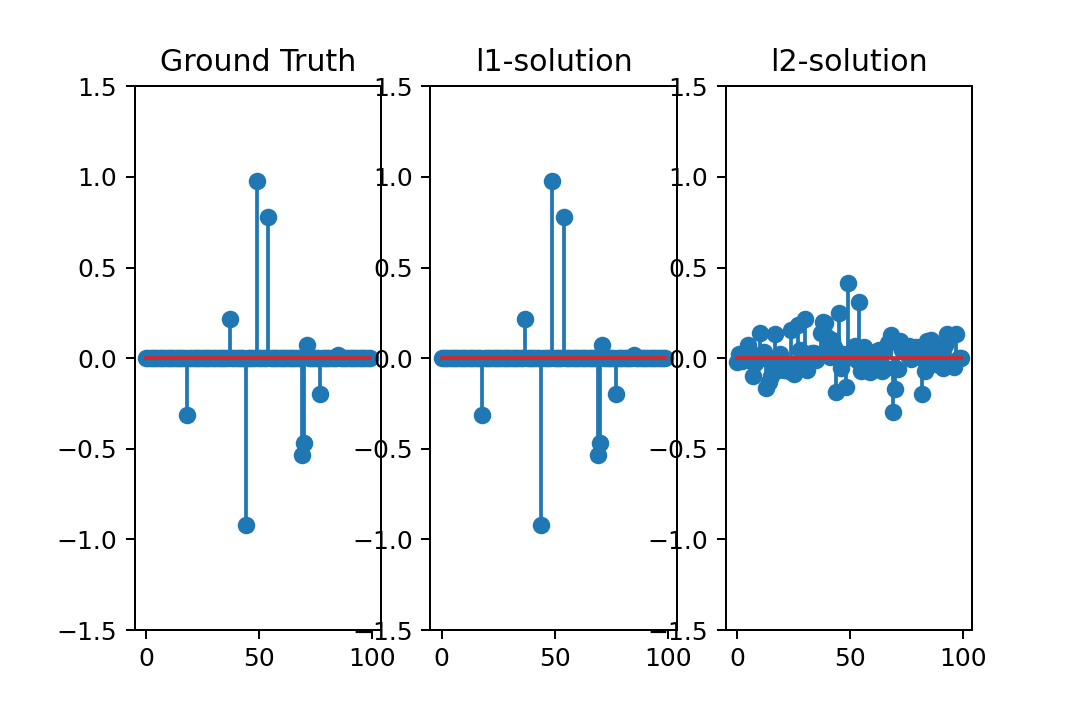
\includegraphics[width=0.5\linewidth]{graphics/l1sol.png}
    \caption{$\ell_1$-regularization and sparsity. The ground truth vector to the left has been 'measured' with a random Gaussian matrix $X$, end then been tried to be recovered with LASSO (middle) and ridge regression (right). The ridge solution is dense and not very close to the ground truth, but the LASSO-solution is essentially equal to the ground trutn.}
    \label{fig:l1sol}
\end{figure}

At first glance somewhat surprisingly, we can however regularize for sparsity by simply changing the regularization norm! This is the idea of the \emph{LASSO} (least absolute shrinkage and selection operator), which amounts to regularizing a linear regression with an $\ell_1$-term:
\begin{align} \label{eq:lasso}
    \min_{\beta} \norm{X\beta-y}_2^2 + \lambda \norm{\beta}_1
\end{align}
The $\ell_1$-norm ('Manhattan norm') is the sum of the absolute norm of the entries of the vector:
\begin{align*}
    \norm{\beta}_1 = \sum_{k \in [p]} \abs{\beta_k}.
\end{align*}
That this works is at first very non-intuitive, but it does work. The solutions of the LASSO are \emph{always} (at most $n$-)sparse (see e.g. \cite[Th.6]{UnserStructure}, or below for a more intuitive argument) and is able to exactly recover an $s$-sparse $\beta_*$ from about $s\log(n)$ measurements (for uncorrelated, centered and bounded features -- we sketch a proof of this later). Ridge regression does not have these properties! See also Figure \ref{fig:l1sol}

There are two things to understand here: 
\begin{itemize}
    \item Why are the solutions sparse?
    \item Why are they equal to the ground truth already after so few observations?
\end{itemize}

\subsubsection{LASSO as a Bayesian method} The knowledge that the ground truth vector $\beta_*$ is sparse can be understood as a \emph{prior} -- a sparse $\beta$ is more likely than a non-sparse one. We can use this intuition to arrive at the LASSO through a \emph{Bayesian approach}.

The idea of Bayesian methods in general is to first choose a \emph{prior} on the \emph{regression weights} $\beta$, and then choose the \emph{most probable} value for $\beta$ conditional on the observations $Y$. That is, we use a maximum likelihood approach:
\begin{align*}
    \max_{b} \mathbb{P}(\beta = b \, \vert \,Y=y)
\end{align*}
To arrive at the LASSO, we impose an \emph{exponential prior} on $\beta$, and assume that the labels have been inflicted with Gaussian noise:
\begin{align}
    &\beta_i \text{ i.i.d exponential, i.e. } \mathbb{P}(\beta = b) = \Pi_{i\in [p]}e^{-\mu\abs{b_i}} \\
    &\mathbb{P}(Y=y\, \vert \, \beta=b) \sim \exp(-\norm{Xb-y}^2_2/2\sigma^2).
\end{align}
Note that the exponential distribution has heavier tails than the Gaussian one. Hence, it is more probable that a few entries of $\beta$ are bigger than the others, which is an approximation of sparsity. One could make other assumptions more closely modeling sparsity, but this would lead to optimization problems which are hard to solve. See the exercises for more information on this!

We then use the Bayes theorem to arrive at $\mathbb{P}(\beta \, \vert \, Y)$:
\begin{align*}
     \mathbb{P}(\beta =b\, \vert \, Y=y) = \frac{\mathbb{P}(Y =y\vert \beta=b)\mathbb{P}(\beta=b)}{\mathbb{P}(Y=y)} \sim \frac{1}{\mathbb{P}(Y=y)}  \exp(-\norm{Xb-y}^2_2/2\sigma^2)\Pi_{i\in [p]}e^{-\mu\abs{b_i}}
\end{align*}
For the optimization over $b$, $\mathbb{P}(Y=y)$ is a constant that can be ignored. It is furthermore equivalent to maximizing something to minimizing its negative logarithm. Hence, maximizing the above over $b$ is equivalent to solving
\begin{align*}
    \min_{b}\tfrac{1}{\sigma^2} \norm{Xb-y}_2^2 + \mu\norm{b}_1,
\end{align*}
which is just another way of writing the LASSO problem.

\paragraph{Remark} We have already seen examples of this approach: LDA and QDA!

\subsubsection{The geometry of the LASSO} There is another, less statistical but more geometrical, may of  understanding the properties of the solutions of the \eqref{eq:lasso}. To simplify the discussion, let us first note that the LASSO can be rewritten to a constrained least squares problem.
\begin{lemma}
    For every $\lambda>0$ exists an $s\geq 0 $ so that the solution of \eqref{eq:lasso} is the same as the $\ell_1$-constrained linear regression problem
\begin{align}
    \min \tfrac{1}{2}\norm{X\beta-Y}_2^2 \text{ subject to } \norm{\beta}_1 \leq s \label{eq:constr}
\end{align}
\end{lemma} 
\begin{proof}
    We will treat the case when \eqref{eq:lasso} has a unique solution. Let $\beta_0$ be that solution and set $s = \norm{\beta_0}_1$. Now let $\beta$ be a vector with $\norm{\beta} \leq s$. Then $\norm{X\beta-Y}_2$ must not be smaller than $\norm{X\beta_0 -Y}_2$ -- otherwise,
    \begin{align*}
        \tfrac{1}{2}\norm{X\beta-Y}_2^2 + \lambda \norm{\beta}_1 < \tfrac{1}{2}\norm{X\beta_0-Y}_2^2 + \lambda \norm{\beta_0}_1, 
    \end{align*}
    which is a contradiction. Therefore, $\beta_0$ solves \eqref{eq:constr}. 

    The only thing left to give a general proof is to show that in any case, all solutions of \eqref{eq:lasso} have the same $\ell_1$-norm. This is possible, but it requires quite involved tools from the theory of convex optimization - we skip this.
\end{proof}

\paragraph{Remark} The lemma shows that we can solve \eqref{eq:constr} instead of the LASSO and obtain the same solutions. If our favorite algorithm works better for one of them, we should hence use that  As the proof shows, there is however no way to a priori tell which $s$ corresponds to which $\lambda$. Since in the end both $\lambda$ and $s$ needs to be tuned, this poses little problems from both the theoretical and practical view.

\smallskip 
The main importance of the  lemma is that we might as well reason about the solutions of \eqref{eq:constr}. And here, we can use geometrical intuition! Let us draw a sketch in two dimensions -- see Figure \ref{fig:l1l2}. Here, we are optimizing over the $\ell_1$-ball, and the function that we are optimizing have level sets that are lines. Those lines will almost always hit the $\ell_1$-ball in one of the vertices. The vertices are exactly the sparse vectors! Compare this to the $\ell_2$-constrained linear regression - the pendant for ridge regression -- here, the lines can hit the circle anywhere.

\begin{figure}
    \centering
    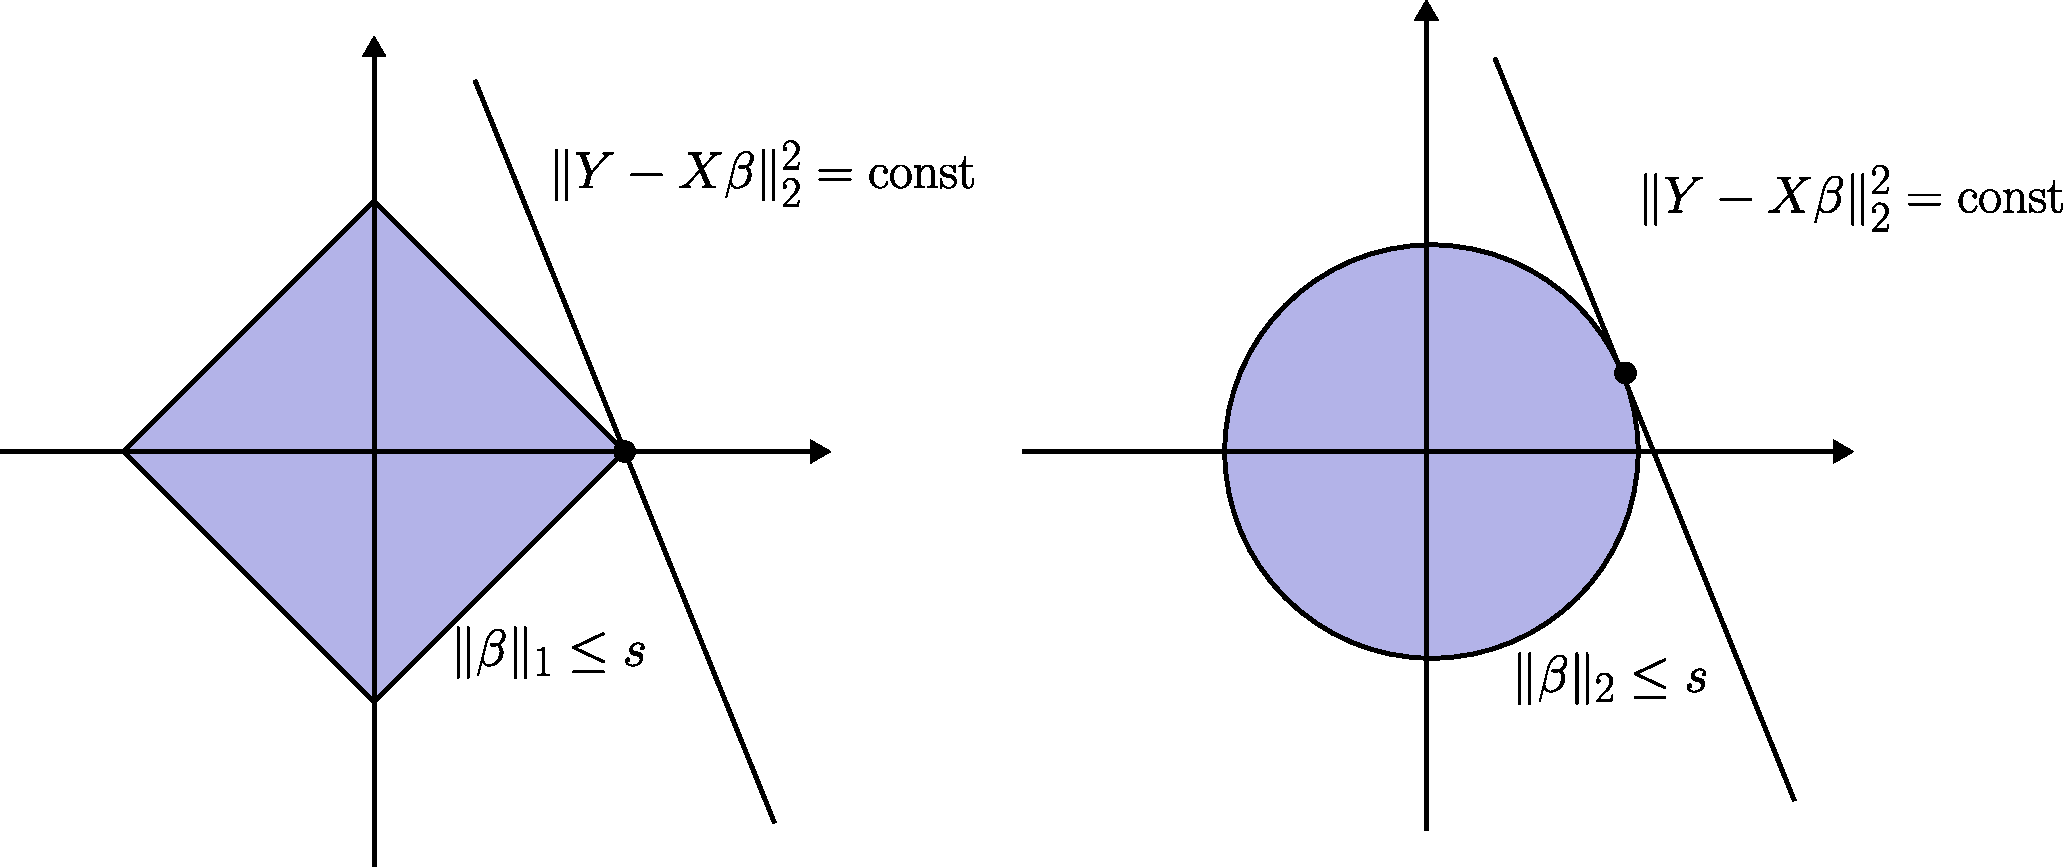
\includegraphics[width=0.75\linewidth]{graphics/l1_vs_l2.pdf}
    \caption{The geometry of LASSO (left) compared to ridge regression (right).}
    \label{fig:l1l2}
\end{figure}

There are ways to formalize this argument and also carry it out in any dimension. In order to understand those argument, we would however first have to take a significant detour into convex geometry and optimization, which would be inappropriate here.

\subsubsection{The low regularization limit: Basis Pursuit} Now let us try to find explainatoin why the LASSO can recover a sparse coeffient vector already from few observations. We will do so in the low-noise, low regularization limit. That is, we will assume that the sparse, linear model is perfect: there exists a sparse $\beta_*$ with $Y= X\beta_*$, and study the limit of LASSO as $\lambda \to 0^+$ (just as we did for ridge regression). Let us begin by making the latter limit more explicit.

\begin{theorem}
    Let $\beta_\lambda$ denote the solution of \eqref{eq:lasso}. Then
    \begin{enumerate}[(i)]
        \item Assume that the following problem has a unique solution $\beta_0$
        \begin{align}
            \min \norm{\beta}_1 \text{ subject to } X\beta = Y. \label{eq:BP}
        \end{align}
        Then, $\lim_{\lambda \to 0} \beta_\lambda = \beta_0$.
        \item $\lim_{\lambda \to \infty} \beta_\lambda = 0$.
    \end{enumerate}

\end{theorem}
\begin{proof}
    This proof will more indirect than the one for ridge regression, because we have no explicit formula here. The argument will on the other hand be more general.

    Let us first deal with (ii), because it is simpler. Notice that trivially, $\beta_\lambda$ has a smaller value of the function that we optimize than $\beta=0$ (since it is optimal). This implies:
    \begin{align*}
        \lambda \norm{\beta_\lambda}_1 \leq \lambda \norm{\beta_\lambda}_1  + \tfrac{1}{2}\norm{X\beta_\lambda - Y }_2^2 \leq \tfrac{1}{2}\norm{Y}_2^2.
    \end{align*}
    Consequently,
    \begin{align*}
        \lim_{\lambda \to \infty} \norm{\beta_\lambda}_1 \leq \lim_{\lambda \to \infty} \tfrac{1}{2}\frac{\norm{Y}_2^2}{\lambda} = 0,
    \end{align*}
    which already shows (ii).
 
    To show (i), we will use two tools from mathematical analysis:
    \begin{itemize}
        \item If a sequence in $\R^p$ is bounded, it has a convergent subsequence.
        \item If a sequence ($\beta_n$) has the property that there exists a $\beta_*$ so that any subsequence of $(\beta_n)$ contains a subsequence convergent to $\beta_*$, the entire sequence converges to $\beta_*$.
    \end{itemize}
    Now, let $\beta_n$ be a sequence of the form $\beta_{\lambda_n}$ for a monotonically decreasing sequence $(\lambda_n)$ with $\lambda_n \to 0$. If we can prove that $\beta_n$ converges to $\beta_0$, we are done.

    Similarly as above, we argue that $\beta_0$ must have a worse optimal value than $\beta_n$. This implies
    \begin{align*}
        \lambda \norm{\beta_n} + \tfrac{1}{2}\norm{A\beta_n- Y}_2^2 \leq \lambda_n \norm{\beta_0}_1 +\tfrac{1}{2}\norm{A\beta_0- Y}_2^2 = \lambda_n\norm{\beta_0}_1,
    \end{align*}
    since $A\beta_0 = Y$. This in particular shows that $\norm{\beta_n}_1 \leq \norm{\beta_0}_1$, i.e. that $\beta_n$ is bounded. Consequently, it must have a convergent subsequence $(\beta_{n'})$, to say $\hat{\beta}$. We immediately see that 
    \begin{align*}
        \norm{\hat{\beta}}_1 = \lim_{n'\to \infty }\norm{\beta_{n'}}_1 \leq \norm{\beta_0}_1
    \end{align*}
    Since also
    \begin{align*}
        \tfrac{1}{2}\norm{A\hat{\beta}-Y} = \lim_{n'\to \infty} \tfrac{1}{2}\norm{A\beta_{n'}- Y}_2^2 \leq \lim_{n'\to\infty}\lambda_{n'} \norm{\beta_0}_1 = 0,
    \end{align*}
    $A\hat{\beta}=Y$. Hence, $\hat{\beta}$ has an $\ell_1$-norm smaller than $\beta_0$ and obeys the constraint -- it hence solves the optimization problem, and $\hat{\beta}=\beta_0$. To finish the proof, we must just note that we can repeat the argument for an arbitrary subsequence of $\beta_n$.
   
\end{proof}

The problem \ref{eq:BP} is called \emph{Basis Pursuit}. Notice the similar relation of the Basis Pursuit to the LASSO as minimal $\ell_2$-norm linear regression to ridge regression.

When does Basis Pursuit recover a $\beta_*$? In the following, we will prove that the following \emph{restricted isometry property} (RIP) is sufficient.
\begin{defi}
    The largest $\delta>0$ so that
    \begin{align*}
        \abs{\norm{X\beta}_2^2 - \norm{\beta}_2^2}< \delta\norm{\beta}_2^2
    \end{align*}
    for all $s$-sparse $\beta$ is called the $s$-Restricted isometry constant of $X$, denoted $\delta_s$. 
\end{defi}
If $\delta_s<1$, we say that $X$ satisfies the $s$-RIP. We will get back to which matrices fulfill the RIP-property.

Why should the RIP imply that LASSO/Basis Pursuit sparse vectors? To see this, let us decipher the condition: It says that $X$ approximately preserves the norm of all $s$-sparse vectors:
\begin{align*}
    \norm{X\beta}_2 \approx \norm{\beta}_2
\end{align*}
This means that if $X$ has the $\delta_{2s}$-RIP, we will have $\norm{X\beta-X\gamma}_2\approx \norm{\beta-\gamma}_2$ for all $s$-sparse vectors. Restricted to them, $X$ hence almost acts as an isometry. In particular, $\norm{X\beta-Y}_2 = \norm{X\beta-X\beta_*}_2 = \norm{\beta-\beta_*}_2$. Thus - and now we're getting \emph{really} handwavy -- the LASSO problem when restricted to $s$-sparse vectors almost turns into the problem
\begin{align} \label{eq:prox}
    \min_\beta \norm{\beta-\beta_*}_2^2 + \lambda \norm{\beta}_1,
\end{align}
which by the above in the Basis Pursuit limit turns into
\begin{align*}
    \min_\beta \norm{\beta}_1 \text{ subject to } \beta=\beta^*,
\end{align*}
which trivially is solved by $\beta^*$. We will need to work more for a valid mathematical argument. See also the exercises.

Now, let us prove a formal theorem instead.
\begin{theorem}
   Suppose that $X$ fulfills the restricted isometry property $\delta_{2s}<\tfrac{1}{3}$. Then, if there exists an $s$-sparse $\beta_*$ so that $X\beta_*=Y$, $\beta_*$ is the unique solution of \eqref{eq:BP}.
\end{theorem}
To give a proof of this result, we need the following technical lemma:
Let us prove a simple lemma.
\begin{lemma}
   % (i) If $\delta_s<1$, all submatrices $X_S$ formed by selecting at most $s$ columns of $X$ will be injective.
    %(ii) 
    For all $s$-sparse $\beta$ and $t$-sparse $\gamma$ whose supports are disjoint, we have
    \begin{align*}
        \abs{\sprod{X\beta,X_\gamma}} \leq \delta_{s+t} \norm{\beta}\norm{\gamma}
    \end{align*}
\end{lemma}
\begin{proof}
    %¤(i) Is simple -- if there is such a submatrix which is not injective, there exists a non-zero $s$-sparse $\beta$ with $X\beta=0$. But then
    %\begin{align*}
    %    0 = \norm{X\beta}_2^2 \geq (1-\delta_s) \norm{\beta}_2^2,
    %\end{align*}
    %which is a contradiction.

    %To prove (ii), 
    First note that it is enough to prove the assertion for the case that $\norm{\beta}_2=\norm{\gamma}_2=1$ -- the more general case follows via scaling. Now consider the \emph{polarization identity}
    \begin{align*}
        \sprod{X\beta,X\gamma} = \frac{1}{4}\left( \norm{X(\beta+\gamma)}_2^2 - \norm{X(\beta-\gamma)}_2^2\right)
    \end{align*}
    Note that $\beta+\gamma$ and $\beta-\gamma$ both are $(s+t)$-sparse. We can therefore estimate the right-hand side with 
    \begin{align*}
        \frac{1}{4}((1+\delta_{s+t})\norm{\beta+\gamma}_2^2 - (1-\delta_{s+t})\norm{\beta- \gamma}^2_2).
    \end{align*}
    Now, since $\beta$ and $\gamma$ are normalized and have disjoint supports, we actually have $\norm{\beta \pm \gamma}_2^2 = \norm{\beta}_2^2+\norm{\gamma}_2^2=2$. Hence, the above is equal to
    \begin{align*}
        \frac{1}{2}((1+\delta_{s+t}) - (1-\delta_{s+t})) = \delta_{s+t} = \delta_{s+t}\norm{\beta}_2\norm{\gamma}_2.
    \end{align*}
\end{proof}
We can now prove that the RIP implies that Basis pursuit recovers $s$-sparse coefficient vectors.


\begin{proof}
   We will prove that if $X$ has the RIP, it has the following \emph{null space property} (NSP): For all $\gamma \in \ker X$ and $S$-sparse support, we have $\norm{\gamma_S}_1<\norm{(\gamma_{S^c})}_1$, where $S^c$ is the complement of $S$. That implies the statement, since if $\beta$ is another vector with $X\beta = Y$, $\beta-\beta_*$ is in $\ker X$. Consequently, with $S=\supp \beta_*$
   \begin{align*}
       \norm{\beta_*}_1 &= \norm{(\beta_*)_S}_1 \leq \norm{\gamma_S}_1 + \norm{\beta_S}_1 \leq \norm{\gamma_{S^c}}_1 + \norm{\beta_S}_1 \\
       &= \norm{(\beta-\beta_*)_{S^c}}_1 + \norm{\beta_S}_1 = \norm{\beta_{S^c}}_1 + \norm{\beta_S}_1  = \norm{\beta}_1.
   \end{align*}
   Hence, any other vector $\beta$ with $X\beta=Y$ has a bigger $\ell_1$-norm, and does not solve the Basis Pursuit.

   To simplify the rest of the proof, let us now make the simple observation that it is enough to prove that 
   \begin{align*}
       \norm{\gamma_S}_2 < \frac{1}{2\sqrt{s}} \norm{\gamma}_1
   \end{align*}
   for all $\gamma \in \ker X$ and $S$ as the indices of the $S$ largest entries in $\gamma$. First, this will trivially show that it holds for all other $s$-sparse supports $S$, and secondly since then
   \begin{align*}
       \norm{\gamma_S}_1 = \sum_{i \in S} \abs{\gamma_i}\cdot 1 \leq \sqrt{\sum_{i \in S} \abs{\gamma_i}^2}\cdot \sqrt{\sum_{i \in S}1  } = \sqrt{s} \norm{\gamma_S}_2 < \frac{1}{2} ( \norm{\gamma_S}_1 + \norm{\gamma_{S^c}}_1),
   \end{align*}
   which can be rearranged to the NSP.

   Now let $\gamma \in \ker X$. Define $S_i$ for $i=0,1,2,\dots$ as the indices of the groups of $s$ largest, next to $s$ largest, $s$ largest after that and so forth entries of $\gamma$, and $\gamma_i := \gamma_{S_i}$ The vector $\gamma_{0}$ is $s$-sparse, and hence, the $RIP$ implies that
   \begin{align*}
       \norm{\gamma_{0}}_2^2 \leq \frac{1}{1-\delta_{2s}} \norm{X\gamma_0}^2
   \end{align*}
   (we could have used $\delta_s$ instead of $\delta_{2s}$ here, but $\delta_{2s}\leq \delta_s$ is trivial, and it will make the rest of the proof cleaner). Now, in light of $X\gamma=0$, we must have $X\gamma_0 = - \sum_{i\geq 1} X\gamma_i$. Hence
   \begin{align*}
       \norm{X\gamma_0}^2 = \sprod{X \gamma_0,X\gamma_0} = - \sum_{i \geq 1} \sprod{X\gamma_0, X \gamma_{i}}.
   \end{align*}
   Now, all $\gamma_i$ are $s$-sparse, and $\gamma_0$ and $\gamma_i$ have disjoint supports. Hence, the lemma implies that $-\sprod{X\gamma_0, X \gamma_{i}} \leq \delta_{2s} \norm{\gamma_0}_2\norm{\gamma_i}_2$, and we can estimate
   \begin{align*}
        - \sum_{i \geq 1} \sprod{X\gamma_0, X \gamma_{i}} \leq \delta_{2s} \norm{\gamma_0}_2 \cdot \sum_{i \geq 1} \norm{\gamma_i}_2.
   \end{align*}
   Now, since all entries in $\gamma_i$ is smaller than the smallest entry in $\gamma_{i-1}$, we can argue
   \begin{align*}
       \norm{\gamma_i}_2 = \left(\sum_{k \in S_i} \abs{\gamma(k)}^2\right)^{\sfrac{1}{2}} \leq\sqrt{s} \max_{k \in S_i} \abs{\gamma(k)} \leq \sqrt{s} \cdot \frac{1}{s}\sum_{k \in S_{i-1}} \abs{\gamma(k)},
   \end{align*}
   i.e. $\norm{\gamma_i}_2 \leq \frac{1}{\sqrt{s}}\norm{\gamma_{i-1}}_1$. Our chain of inequalities can now be boiled down to
   \begin{align*}
         \norm{\gamma_{0}}_2^2 \leq \frac{\delta_{2s}}{1-\delta_{2s}} \cdot \frac{1}{\sqrt{s}} \sum_{i \geq 1} \norm{\gamma_{i-1}}_1 < \frac{1}{2\sqrt{s}} \norm{\gamma}_1
   \end{align*}
   if $\frac{\delta_{2s}}{1-\delta_{2s}}< \tfrac{1}{2}$, which is equivalent to $\delta_{2s}<\tfrac{1}{3}$.
\end{proof}

\paragraph{Remark} One can also prove versions of the above theorem which handles the case $Y=X\beta_*+\calE$ for some moderately small $\calE$-- see \cite[Sec. 5.3]{FouRau2013}.



\subsubsection{Matrices with the RIP}
Now we know that the RIP implies that Basis Pursuit (and to some extent as a consequence, the LASSO) will be able to recover any $s$-sparse ground truth $\beta_*$. But what $X$ have the RIP?

First, one can use something called the \emph{Gershgorin circle theorem} to show that if $X$ has normalised columns and a mutual coherence $\mu < \tfrac{\delta}{s-1}$, all matrices of the form $X_S^*X_S$  have eigenvalues between $(1-\delta)$ and $(1+\delta)$, which is equivalent to the RIP. As we already discussed though, to have a mutual coherence of that small magnitude, we need $n\gtrsim s^2$ measurements. This 'resistance to mutual-coherence-based arguments' to prove a RIP for matries with less than $s^2$ measurements is colloquially referred to as the \emph{square-root bottleneck}: using mutual coherence, a matrix with $n$ rows can only be shown to be able to recover $\sqrt{n}$-sparse $\beta_*$

It has been proven to be extremely hard to design \emph{deterministic} matrices that break the square-root bottleneck. Using extremely complicated combinatoric arguments, \cite{bourgain2011explicit} were the first authors to do so. As late as 2022, a subset of the authors published an improved paper \cite{ford2022explicit} using recent developments in combinatorics. But even this updated version only manages to get an $s$-RIP using $n\sim s^{\sfrac{2}{(1+\epsilon)}}$, measurements with $\epsilon=1.63\cdot 10^{-7}$.

However, using \emph{random matrices}, one can do \emph{a lot} better. For many different constructions, it turns out that only 
\begin{align*}
    n \gtrsim s\log(p)
\end{align*}
is necessary to get the $(2)s$-RIP. Many constructions use the following about the distribution of $X$:
\begin{itemize}
    \item The rows of the matrix are \emph{independently} drawn. 
    \item The rows of $X$ are bounded -- $\norm{x}$ is bounded by some constant almost surely, or it at least decays as a Gaussian (one speaks of \emph{sub-Gaussian} distributions). 
    \item The features are normalized and uncorrelated -- that is, $\mathbb{E}(x(k)x(j))=\delta_{kj}$.
\end{itemize}
The first one of these assumptions makes a lot of sense from a statistical point of view --  it just means that our data vectors $x_i$ are drawn independently, which is the standard assumption in all machine learning. The latter two are however more questionable -- let us get back to that.

The claim is now the matrix $\tfrac{1}{\sqrt{n}}X$ (the factor is to make sure that the columns of the matrix are close to one with high probability) has the $s$-RIP with high probability for $n \geq C s\log(p)$, where $C$ is some numerical constant. Let us sketch a proof in the simplest of cases, namely that the features are i.i.d. $\mathcal{N}(0,1)$-distributed. That is, all entries in $X$ are i.i.d. Gaussian -- one speaks of a \emph{Gaussian matrix}. We will hide quite many painfully technical details, but we will see all important ideas, that can be generalized to other matrices. The details can be found in \cite[Ch. 9.1]{foucart2011hard}.

\paragraph{Step 1: Concentration of a single vector} Note that what we want to prove that $\norm{X\beta}_2^2 \approx \norm{\beta}_2^2$ for all $s$-sparse $\beta$. In fact, it is enough to show that only for sparse vectors with norm at most one, since other vectors can be dealt with with scaling. Let us call the latter set $\calS$.

Now let's start by showing that we have such an approximate equality for \emph{each fixed} $\beta\in \calS$. Notice that  $\tfrac{1}{\sqrt{n}} X\beta = \sum_{i} \beta_i X^i$ is a sum of independent Gaussians, and hence a Gaussian itself. Its coherence matrix has entries
\begin{align*}
    \mathbb{E}((X\beta(X\beta)^*)_{ij}) = \sum_{i,j,k,\ell} \mathbb{E}(x_i(k) \beta(k) x_j(\ell) \beta(\ell)) =  \sum_{i,j,k\ell} \delta_{ij}\delta_{k\ell} \beta(k) \beta(\ell) = \norm{\beta}_2^2 \delta_{ij}.
\end{align*}
Hence, $\frac{1}{\norm{\beta}}X\beta$ is a standard normal Gaussian $n$-dimensional vector. The norms of such vectors $g$ concentrate around its mean $n$ -- i.e, $\mathbb{P}( \abs{\norm{g}_2^2 - n}> \epsilon)$ is small. Using this fact, we obtain the following
\begin{theorem}
    There exists a constant $c$ independent of $n$ and $p$ such that for a Gaussian $X$, we have for any fixed $\beta$
    \begin{align}
        \mathbb{P}(\abs{\frac{1}{n} \norm{X\beta}_2^2 - \norm{\beta^2}} >t\norm{\beta}^2_2) \leq 2\exp(-cnt^2). \label{eq:conc}
    \end{align}
\end{theorem}

\paragraph{Step 2: Concentration on a net means concentration everywhere}
The next step is to realize that if we have $\norm{X\beta}_2^2 \approx \norm{\beta}_2^2$ for all $\beta$ in a so-called $\epsilon$-net of the set of sparse vectors of norm at most one, i.e. a set $(\beta_i)_{i \in T}$
\begin{align*}
    \sup_{\beta \text{ s-sparse}} \min_{i \in T} \norm{\beta-\beta_i}_2 \leq \epsilon,
\end{align*}
that can subsequently be extended to the entire set of sparse vectors with norm smaller than one. Concretely , one has the following
\begin{theorem}
    Suppose that $\abs{\frac{1}{n} \norm{X\beta_i}_2^2 - \norm{\beta_i}^2} \leq t\norm{\beta_i}_2^2$ for all $\beta_i, i \in T$ for an $\epsilon$-net of the set of sparse vectors. Then, it has $\delta_s \leq \frac{t}{1-2\epsilon}$.
\end{theorem}

\paragraph{Step 3: Concentration on a net} We conclude that in order to get $\delta_s \leq \delta = \tfrac{\delta/2}{1-2\cdot\tfrac{1}{4}}$, we need to secure that the probability that 
\begin{align*}
    \sup_{i \in T} \abs{\frac{1}{n} \norm{X\beta_i}_2^2 - \norm{\beta_i^2}} >\tfrac{\delta}{2}\norm{\beta_i}^2_2
\end{align*}
is small for a $\tfrac{1}{4}$-set. We can however immediately invoke \eqref{eq:conc} together with a trivial union bound to obtain
\begin{align}
    \mathbb{P}\left( \sup_{i \in T} \abs{\frac{1}{n} \norm{X\beta_i}_2^2 - \norm{\beta_i^2}} >\frac{\delta}{2}\norm{\beta_i}^2_2 \right) \leq 2\abs{T}\exp(-cn\delta^2/4). \label{eq:netrip}
\end{align}
It is thus now only left to investigate how large we need to choose $T$ in order to get an $\tfrac{1}{4}$-net of $\calS$. For this, we envoke the theory of \emph{covering numbers}. First, let us fix a support $S$ and look at the set $\{x : \supp x \sse S, \norm{x}_2 \leq 1\}$. One can prove [FouRau, Prop .3] that it is possible to find a $t$-net for that set with no more than $(1+\frac{2}{t})^s$ vectors, i.e. $9^s$ to get a $\tfrac{1}{4}$-net. If we now choose one net per such support and combine them, we get a net for all of $\mathcal{S}$. Since there are $\binom{p}{s}\leq p^s$ such supports, we conclude that we may choose a net of size smaller than $(9p)^s$, and the probability in \eqref{eq:netrip} is smaller than
\begin{align*}
    2(9p)^s\exp(-cn\delta^2/4) <\varepsilon
\end{align*}
if 
\begin{align*}
    n \gtrsim \frac{4}{\delta^2}(s\log(9p) + \log(\tfrac{2}{\epsilon})),
\end{align*}
which is the claim.



\subsubsection{Is the RIP a realistic assumption? Necessary?} Now let us get back to our set of assumptions. Are they reasonable? The boundedness assumption is in some situations problematic -- distributions in real life can have heavy tails -- but is still quite 'cheap' to assume. The correlation assumption is however very naive to make -- in real datasets, there are often features that are highly correlatied.

Sadly, the decorrelation assumption is not only sufficient, but also some extent also necessary -- if there are two features that are perfectly correlated, $x(k)=x(j)$, we will have for $\beta$ with $\beta(k)=\beta(j)= \tfrac{1}{\sqrt{2}}$ and all other coefficients zero
\begin{align*}
    \norm{X\beta}_2^2 = \sum_{i \in [n]} ( \frac{x_i(k)+x_i(k)}{2})^2  = 2 \sum_{i\in [n]}\abs{x_i(k)}^2 = 2 \norm{X^k}^2.
\end{align*}
In order for the RIP to hold, that $k$:th column of $X$ needs to be normalized. $\beta$ is hence a $2$-sparse vector with norm $1$ and $\norm{X\beta}_2^2=2\norm{\beta}_2^2$-- we have no RIP.

We therefore have to, sadly, conclude that  in practice, many matrices do not have the RIP. Does that mean that the LASSO and Basis pursuit is not applicable in practice? Yes and no.
\begin{itemize}
    \item If our main concern is to find the sparse coefficient vector $\beta_*$, we can say that we will almost certainly fail if the features are correlated. Or in other words, we have to be very careful to draw conclusions of which features are important simply by looking at the LASSO estimate $\beta$. There may for instance be important features that are not chosen simply because LASSO chooses another, correlated feature instead.
    \item If we however are only concerned with building a good predictor, this should not concern us too much. The results above are all about the recovery of the correct $\beta$, and say very little about the test error. Just as for ridge regression, an incorrect $\beta$ can still give very good test loss for certain data distributions! 
\end{itemize}

If one is in a situation with highly correlated features, one might want to use the \emph{elastic net} instead of the LASSO. Conceptually, it is simple: We add a combination of the $\ell_1$ and $\ell_2$-regularizers to our linear regression:
\begin{align*}
    \min_{\beta} \tfrac{1}{2}\norm{X\beta-Y}_2^2 + \lambda_1 \norm{\beta}_1 + \lambda_2 \tfrac{1}{2}\norm{\beta}_2^2
\end{align*}
If there are highly correlated features that explain $Y$ well, the elastic net will put similar weights on them, whereas the LASSO will only pick one of them. We will not get into more theoretical detail than that - the interested reader is instead referred to \cite{zou2005regularization}


\subsection{Recommended reading and exercises}
Chapter 6, in particular sections 6.1, 6.2 and 6.4 of \href{https://www.statlearning.com/}{An introduction to Statistical Learning} is good reading about linear regression in high dimensions. For a more detailed proof of Gaussian matrices having the RIP, see \cite{baraniuk2008simple}. The mathematical theory of sparse regression is called \emph{Compressed sensing}, or sometimes also \emph{compressive sensing}.

\smallskip

Recommended exercises in An introduction to Statistical learning are 6.1, 6.2, 6.3, 6.4, 6.5.
\smallskip

Also consider these questions (some of which are from \cite{foucart2011hard}):

\begin{exercise}
    Suppose that a matrix $X$ with normalized columns has a low 'local' mutual coherence on a set $J$, i.e. $\sup_{i,j \in J, i\neq j} \abs{\sprod{X^i,X^j}} \leq \widehat{\mu}$ with $\widehat{\mu}$ significantly lower than the mutual coherence $\mu(X)$ of the entire matrix. If $\widehat{\mu}\leq \tfrac{1}{2s-1}$, is it guaranteed that any $s$-sparse $\beta$ with $\supp \beta \sse J$ will be recovered by OMP? Explain your answer.
\end{exercise}

\begin{exercise}
    Show that ridge regression can be viewed as a Bayesian maximum likelihood estimate if we but a Gaussian prior on the $\beta$-parameter.
\end{exercise}

\begin{exercise}
    The exponential prior does not make exactly sparse vector likely. One could argue that the following prior is better suited: For some $p>0$,
    \begin{align*}
        \beta_i=\sim \mu \pi_i , \pi_i \sim\mathrm{Ber}(p) \text{ i.i.d.}.
    \end{align*}
    That is, to assume that the entry is nonzero with a probability $p$, and if it is nonzero, it is equal to a constant $\mu$.
    \begin{enumerate}[(a)]
        \item Show that the maximum likelihood estimate can be obtained through
        \begin{align*}
            \min_{\beta} \tfrac{1}{\sigma^2} \norm{X\beta-Y}_2^2 + p \abs{\mathrm{supp(\beta)}}
        \end{align*}
        \item Why is this method not used? (Think practically)
    \end{enumerate}
\end{exercise}

\begin{exercise}
    Sometimes, it is reasonable to assume that certain indices $i$ is more likely to have non-zero parameters $\beta(i)$. One can then use the \emph{weighted} LASSO:
    \begin{align*}
        \min_{\beta} \norm{X\beta-Y}_2^2 + \lambda \cdot \sum_{i\in [d]} w_i\abs{b_i}.
    \end{align*}
    Here, $w_i>0$ are weights (which are hyperparameters).
    \begin{enumerate}[(a)]
        \item Argue that the weighted LASSO is a Bayesian maximum likelihood estimate: The prior is $\mathbb{P}(\beta_i=b)\sim \exp(-\mu_i \abs{b})$, where $\mu_i$ is different for all $i$.
        \item If a parameter is likely to be zero, should the $w_i$ be chosen small or big? Discuss this also in relation to $(a)$.
    \end{enumerate} 
\end{exercise}

\begin{exercise}
    Consider the $\ell_\infty$-norm $\norm{\beta}_\infty = \max_{i} \abs{\beta_i}$ and the optimization problem 
    \begin{align}
        \min \norm{X\beta - Y} + \lambda \norm{\beta}_\infty \label{eq:linfty}
    \end{align}
    \begin{enumerate}[(a)]
        \item Discuss the limits $\lambda \to 0^+$ and $\lambda \to \infty$.
        \item What will solutions of \eqref{eq:linfty} look typically like? Justify your answer.
    \end{enumerate}
\end{exercise}

\begin{exercise}
    A popular class of RIP matrices are so-called \emph{BOS}-matrices (bounded orthonormal systems). They are formed via randomly drawing $n$ rows out of a fixed unitary matrix $U$, i.e. a matrix with $U^TU=I$, with $I$ the identity matrix.

    By considering the identity matrix, argue that this does not always yield a RIP matrix with $m<p$. 
    
    \emph{Remark:} To actually obtain a matrix with the RIP, one can assume that the vectors $u_i \in \R^p$ have small entries (proportional to $p^{-1/2}$) in modulus.
\end{exercise}

\begin{exercise}
    Assume that $X$ is a data matrix so that (for a fixed $\lambda>0$), the Ridge regression minimizer $f(y)$ is unique for every value of $y \in \R^n$. Show that the map $f$ is continuous. 
\end{exercise}

\begin{exercise}
    Repeat the last exercise, but for the LASSO minimizer instead. (\emph{Hint}: This is considerably trickier)
\end{exercise}

\begin{exercise}
    Prove that if nullspace of $X$ contains a $2s$-sparse vector $\beta_0$ (i.e. $X\beta_0=0$), there exists an $s$-sparse vector $\beta_1$ which is not recovered by Basis pursuit (that is, when solving it with $Y=X\beta_1$, $\beta_1$ is not the unique solution).
\end{exercise}

\begin{exercise}
    Given a matrix $X$, are the RIP constants of the matrix $tX$ for every $t$ the same? 
\end{exercise}



\begin{exercise}
    The purpose of this exercise is to prove the Welch bound. Let $X \in \R^{n,p}$ be a matrix with normalized columns.
    \begin{enumerate}[(i)]
        \item Let $G= X^TX$. Argue that $G$ has at most $n$ non-zero eigenvalues. From this, show that the eigenvalues $\lambda_i$ of $G$ obeys
        \begin{align}
            \sum_{i \in [p]} \lambda_i \leq \sqrt{n} \cdot \sqrt{\sum_{i \in [p]} \lambda_i^2} \label{eq:welch1}
        \end{align}
        \item Using that the sum of the eigenvalues of a diagonalizable matrix $A$ is equal to its trace $\tr(A) = \sum_i A_{ii}$, argue that $G$:s eigenvalues obeys
        \begin{align}
            \sum_{i \in [p]} \lambda_i = p \label{eq:welch2}
        \end{align}
        \item Using that the sum of the squares of the eigenvalues of a matrix $A$ equals its Frobenius norm squared $\norm{A}_F^2= \sum_{i,h} \abs{A_{ij}}^2$, argue that
        \begin{align}
            \sum_{i \in [p]} \lambda_i^2 \leq p + p(p-1)\mu(X)^2 \label{eq:welch3}
        \end{align}
        \item Derive the Welch bound from \eqref{eq:welch1}, \eqref{eq:welch2} and \eqref{eq:welch3}
    \end{enumerate}
\end{exercise}

\begin{exercise}
    Suppose that we know a priori that the $s$-sparse coefficient vector $\beta_*$ we wish to recover from $Y=X\beta_*$ has the property that its support is contained in a set $\mathcal{B}$ with $\abs{\mathcal{B}}\leq \tilde{p}<p$.
    \begin{itemize}
        \item Formulate an adapted form of the LASSO for estimating $\beta$.
        \item Suppose that $X$ is a Gaussian matrix. How many rows will it need for your new version of LASSO to succeed? Justify your answer.
    \end{itemize}
\end{exercise}

\begin{exercise}

    Let $\varsigma_\lambda: \R^p \to \R^p$ denote the \emph{soft thresholding operator}:
  
    \begin{picture}(300,100)
         \put(50,50){$
        \varsigma_\lambda(\gamma)_i = \begin{cases}
            x_i-\lambda &\text{ if } x_i > \lambda \\
            0 &\text{ if } \abs{x_i}\leq\lambda \\
            x_i + \lambda &\text{ if } x_i<-\lambda
        \end{cases} $}
        \put(250,10){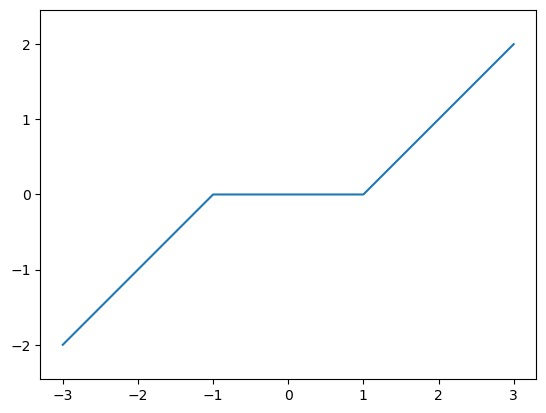
\includegraphics[width=0.25\textwidth]{graphics/soft_threshold.png}}
    \end{picture}

    Show that the problem \eqref{eq:prox} is solved by $\varsigma_\lambda(\beta_*)$. Argue that this implies that the solution of \eqref{eq:prox} will be very (i) close to the ground truth (ii) sparse if the ground truth is. 

\end{exercise}



\section{Unsupervised learning -- Clustering methods}  
We have up until now been concerned with supervised learning, i.e. settings where we are given data with labels, and try to find functions that estimate the labels on unseen data.

We now want to discuss a few selected methods in \emph{unsupervised learning}. In unsupervised learning, we are given data and are tasked with finding 'patterns' in it. Already from the formulation of the problem, we see that it is much less ill-defined than the supervised setting. What does it mean to find a 'pattern'? To make it a bit more concrete, let us say that we want to determine \emph{clusters} in the data -- i.e., subsets $S_k\sse [n]$ so that the points $x_i$, $i\in C_k$ are ''similar'', but points from different clusters are ''dissimmilar''.

\paragraph{Remark:} Since the clustering problem is less well-defined than the supervised one, it is in general hard to evaluate a clustering method -- we by definition have no right answer! We can evaluate our methods on datasets where we have ground-truth classes, and see if the methods can identify those classes, but there is in general not much more we can do. Clustering methods should therefore be used rather in an exploratory manner: they can help us finding patterns in the data, but these patterns should rather be treated as starting points for further studies than anything else. \newline

\subsection{K-means/medoids/Kernel K-means}
We have in fact already encountered an 'ad-hoc' clustering method: calculating and then plotting the principal components of the data in two dimensions and then simply look look at it. If the data is non-uniformly distributed, we may be able to visually determine regions where groups of examples are concentrated. Such groups are clusters. 

How can we automatically find such groups? As we said earlier, the ultimate goal is to find subsets of the data with \emph{similar data}. If they are similar, we should be able to find a point $m$ that has a small average distance to the points in $C_k$. That is,
\begin{align}
    W(C_k) = \min_{m\in \R^p} \sum_{i \in C_k} \dist(x_i,m) \label{eq:means}
\end{align}
should have a small value. It is then a reasonable idea is to try to minimize
\begin{align} \label{eq:cluster}
    \min_{C_0, \dots, C_{K-1}} \sum_{k \in [K]} W(C_k).
\end{align}
One should note here that we have fixed the number of clusters here to be equal to $K$ (which of course is a tuneable) and that we optimize over clusters which are disjoint $C_i \cap C_j=\emptyset$, and encompass all data $\cup_{k} C_k = \{x_i, i \in [n]\}$.

It is not feasible to solve \eqref{eq:cluster} directly -- there are simply too many clusters to test. There is however a simple, iterative way to at least find a local minimum
\begin{enumerate}
    \item For fixed clusters, find the 'representatives' $m_k$ that solve the problems \eqref{eq:means}
    \item Reassign the points $x_i$ to the cluster $C_k$ so that $\dist(x_i,m_k)$ is minimal.
    \item Repeat.
\end{enumerate}


\paragraph{$K$-means} 
In general, step (1) cannot be resolved. If we however used the squared Euclidean distance as a distance, it however can -- it is not hard to show that the minimum is given by the \emph{centroid} of the cluster
\begin{align*}
    \argmin_{m\in \R^p} \sum_{i \in C_k} \norm{x_i-m}_2^2 = \frac{1}{\abs{C_k}}\sum_{i \in C_k}x_i.
\end{align*}
This leads to the so-called \emph{$K$-means algorithm}.


\begin{algorithm}[tb]      
	\caption{$K$-means} 
	\label{alg:kmeans}
	\begin{algorithmic} [1]
 		\REQUIRE Training data $x_i$.
 		\STATE Randomly assigned clusters $C_i$.
 		\REPEAT
 			\STATE Calculate centroids
            \begin{align*}
                m_k = \frac{1}{\abs{C_k}}\sum_{i \in C_k}x_i.
            \end{align*}
            \STATE Re-assign all points $x_i$ to the cluster $k$ so that $\norm{x_i-m_k}$ is minimal.
 		\UNTIL Clusters no longer change.
 		\RETURN Clusters $C_i$.
	\end{algorithmic}
\end{algorithm}

\paragraph{$K$-medoids} Another way to assign the $m_k$ is to find the point \emph{within each cluster} that minimizes \eqref{eq:means}, i.e.
\begin{align*}
    m_k^* = \argmin_{x \in C_k} \sum_{i\in C_k} \dist(x_i,x).
\end{align*}
As long as the clusters are relatively small, this relatively cheap. This policy leads to the \emph{$K$-medoids} algorithm. 

When applied to the euclidean squared distance, $K$-means and $K$-medoids typically lead to very similar results. The interest in $K$-medoids is instead that it can be applied to non-euclidean data and distances. For instance, the features can be qualitative, and the distance between two points defined as the number of qualitative features that are not equal!


\begin{algorithm}[tb]      
	\caption{$K$-medoids} 
	\label{alg:kmedoids}
	\begin{algorithmic} [1]
 		\REQUIRE Training data $x_i$.
 		\STATE Randomly assigned clusters $C_i$.
 		\REPEAT
 			\STATE Calculate 'medoids'
            \begin{align*}
                m_k = \argmin_{x \in C_k} \sum_{i\in C_k} \dist(x_i,x).
            \end{align*}
            \STATE Re-assign all points $x_i$ to the cluster $k$ so that $\dist(x_i,m_k)$ is minimal.
 		\UNTIL Clusters no longer change.
 		\RETURN Clusters $C_i$.
	\end{algorithmic}
\end{algorithm}

\paragraph{Kernel $K$-means} A more mathematically interesting alternative to $K$-means is the kernel version of $K$-means. Similarly as with SVMs, we imagine that we perform $K$-means on data that we have transformed into a higher-dimensional feature space $\calH$ using a non-linear map $\varphi:X \to \calH$. We would then obtain centroids
\begin{align*}
    \mu_k = \frac{1}{\abs{C_k}}\sum_{i \in C_k} \varphi(x_i).
\end{align*}
Now, in order to re-assign a point to a cluster, we would need to minimize $\norm{\varphi(x_i)-\mu_k}_\calH$ over $k$. Since however
\begin{align*}
    \norm{\varphi(x_i)-\mu_k}_\calH^2 =& \sprod{\varphi(x_i),\varphi(x_i)} - 2 \sprod{\varphi(x_i), \mu_k} + \sprod{\mu_k,\mu_k} \\
     =&  \sprod{\varphi(x_i),\varphi(x_i)} - 2 \sprod{ \varphi(x_i), \frac{1}{\abs{C_k}}\sum_{j \in C_k} \varphi(x_j)} \\
    &+ \sprod{\frac{1}{\abs{C_k}}\sum_{j \in C_k} \varphi(x_j),\frac{1}{\abs{C_k}}\sum_{j \in C_k} \varphi(x_j)} \\
    &= \sprod{\varphi(x_i),\varphi(x_i)} - \frac{2}{\abs{C_k}}\sum_{j \in C_k} \sprod{\varphi(x_i),\varphi(x_j)} + \frac{1}{\abs{C_k}^2} \sum_{j,\ell\in C_k} \sprod{\varphi(x_j),\varphi(x_\ell)}
\end{align*}
we see that all calculation again can be performed without explicitly calculating $\varphi$, and only work with the inner products $\sprod{\varphi(x_i),\varphi(x_j)}$ given by a kernel $\mathcal{K}$. The resulting method is called Kernel $K$-means.

    \begin{algorithm}[tb]      
	\caption{Kernel $K$-means} 
	\label{alg:kernelkmeans}
	\begin{algorithmic} [1]
 		\REQUIRE Training data $x_i$, kernel $\mathcal{K}$.
 		\STATE Randomly assigned clusters $C_i$.
 		\REPEAT
 			\STATE  Re-assign all points $x_i$ to the cluster $k$ so that 
    \begin{align*}
        \mathcal{K}(x_i,x_i)  - \frac{2}{\abs{C_k}}\sum_{j \in C_k} \mathcal{K}(x_i,x_j) + \frac{1}{\abs{C_k}^2} \sum_{j,\ell\in C_k} \mathcal{K}(x_j,x_\ell).
    \end{align*}
    is minimal
 		\UNTIL Clusters no longer change.
 		\RETURN Clusters $C_i$.
	\end{algorithmic}
\end{algorithm}

\subsection{Hierarchical Clustering}
Two weaknesses of the $K$-means/medoids algorithms are that (i) the number of clusters needs to be pre-defined (ii) after clustering, we have little overview of how close clusters are linked to each other. \emph{Hierarchical clustering} solves these issues. Hierarchical clustering builds a decision tree where the leaves correspond to clusters. While it is possible to build these by succesively dividing the clusters, as with decision trees (interested readers should read up on the DIANa algorithm \cite{patnaik2016divisive}), the more simple approach\footnote{In short, the problem with building from the top is that there are too many possibilites. There are $2^n$ alternatives for the first split when $n$ points are used!} is to build from the bottom-up, i.e. starting with $n$ one-example clusters, and then fusing them. This is referred to as \emph{agglomerative clustering}.

The algorithm functions as follows: We initialize a graph with $n$ nodes, each corresponding to a datum, and no edges. This can be seen as a 'forest graph' with $n$ smaller trees. We iteratively fuse these trees by adding edges and nodes until we end up with a  single tree.  To decide which trees to combine, at each step, we consider all pairs of trees, which correspond to clusters $C_i, C_j$ in the data, and measure the 'dissimilarity' of the \emph{combined cluster} $L(C_i,C_j)$. The pair with the smallest dissimilarity are then fused, i.e. connected with a new parent node in the graph that we are building. The algorithm is summarized in Algorithm \eqref{algo:aggcluster}

The dissimilarity measure $L$ is often referred to as \emph{linkage} in this context. There are many different linkage functions -- here are a few of the. They each assume that we have access to a simple distance measure $\dist$ between data points.
\begin{itemize}
    \item Complete: the linkage is the maximal pairwise distance between points in the clusters.
    \begin{align}
        L(C_i,C_j) = \max_{x \in C_i,x'\in C_j} \dist(x,x').
    \end{align}
    In this way, clusters are only fused if all points in $C_i$ are close to all points in $C_j$.
    \item Single: the linkage is the minimal pairwise distance between points in the clusters.
    \begin{align*}
        L(C_i,C_j) = \min_{x\in C_i,x'\in C_j} \dist(x,x').
    \end{align*}
    In this way, clusters are fused when there is one good ''connecting pair'' of points. .
    \item Average: The linkage is the average pairwise distance between points in the clusters.
    \begin{align*}
        L(C_i,C_j) = \tfrac{1}{\abs{C_i}\abs{C_j}}\sum_{x\in C_i,x'\in C_j} \dist(x,x').
    \end{align*}
    Here, clusters are fused when many points in $C_j$ are close to many points in $C_i$, but there is some tolerance for outliers.
    \item Centroid: Here, we keep track of a centroid/median/'representative point' for $m_k$ for each cluster, and use the distance between those is the linkage
    \begin{align*}
        L(C_i,C_j) = \dist(m_i,m_j).
    \end{align*}
    \item 'Ward': The linkage of the clusters is equal to the difference between the variance of the combined cluster with the variances of the individual clusters, weighted with cluster size. In formulas:
        \begin{align*}
            L(C_i,C_j) = \sum_{x \in C_i \cup C_j} \norm{x-m_{C_i\cup C_j}}^2 - \sum_{x \in C_i} \norm{x-m_{C_i}}^2 - \sum_{x \in C_i} \norm{x-m_{C_j}}^2, 
        \end{align*}
        where $m_C$ is the mean of the datapoints in the cluster $C$. It is only defined for Euclidean data, and is the default in sklearn. It is in fact quite cheap to calculate: it is in fact equal to 
        \begin{align} \label{eq:ward_linkagew}
            \frac{\abs{C_i}\abs{C_j}}{\abs{C_i}+\abs{C_j}} \norm{m_{C_i}-m_{C_j}}^2.
        \end{align}
\end{itemize}
Which method is 'best' depends on the data, and is best evaluated empirically. Complete and average linkage tend to lead to more 'even' clusters compared to single linkage, where new clusters are formed by just adding one new point to it. Centroid linkage is very cheap (since only one distance needs to be calculated when evaluating the linkage), but does not have the following, nice property:
\begin{align} \label{eq:monotonicity}
    L(C_i \cup C_j,C_k) \geq \min (L(C_i,C_k), L(C_j,C_k)).
\end{align}
This property is nice since it makes the \emph{dendrograms} of the hierarchies more interpretable. A dendrogram is formed when laying out the tree in a way so that the $y$-coordinate of a node $C_k$ is equal to its similiarity measure $\lambda_k$ (See Algorithm \ref{algo:aggcluster}). \eqref{eq:monotonicity} implies that parents always are higher situated than children in that plot, meaning that 'lower situated subclusters' are always less dissimilar than higher connected clusters. This property also implies that for any maximal similarity measure we choose, we form clusters by cutting the trees at that level, as shown in Figure \ref{fig:dendro}.

\begin{algorithm}[tb]     
	\caption{Agglomerative hierarchical clustering \label{algo:aggcluster}} 
	\begin{algorithmic} [1]
 		\REQUIRE Data $X$, similarity measure $W$
 		\STATE Initialize $n$ trees $C_i$ with a single node containing one datum $x_i$.
 		\REPEAT
 			\STATE Find the pair $C_i,C_j$ of current trees that minimizes $L(C_i,C_j)$. 
            \STATE Fuse these trees by connecting them to a new parent node $C_{k}=(C_i \cup C_j)$, and (optionally) record $\lambda_k =L(C_i, C_j) $
 		\UNTIL Only one tree left
 		\RETURN Clusters $C_k$, (optionally) similarity measures $\lambda_k$.
	\end{algorithmic}
\end{algorithm}

\begin{figure}
    \centering
    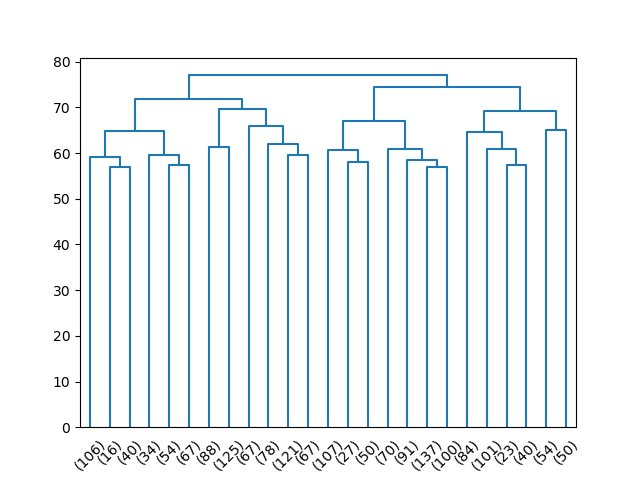
\includegraphics[width=0.24\linewidth]{graphics/dendrogram_complete.png}  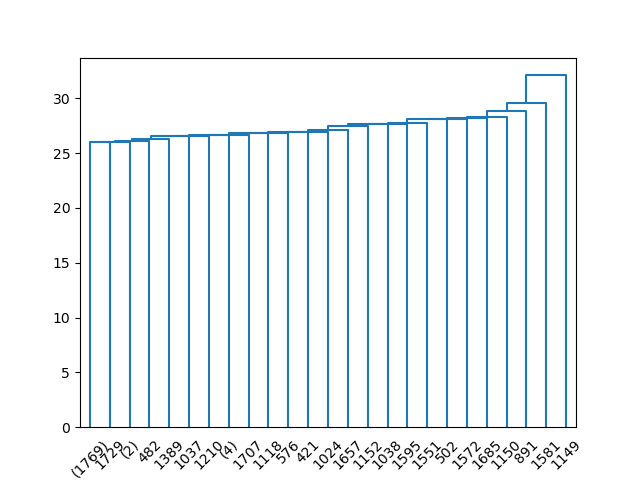
\includegraphics[width=0.24\linewidth]{graphics/dendrogram_single.png} 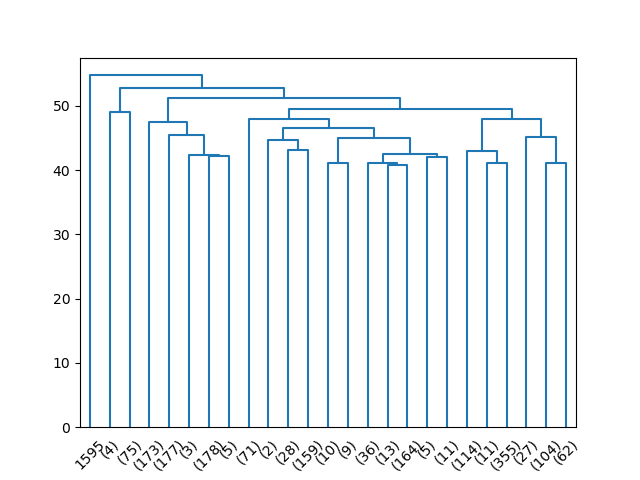
\includegraphics[width=0.24\linewidth]{graphics/dendrogram_average.png}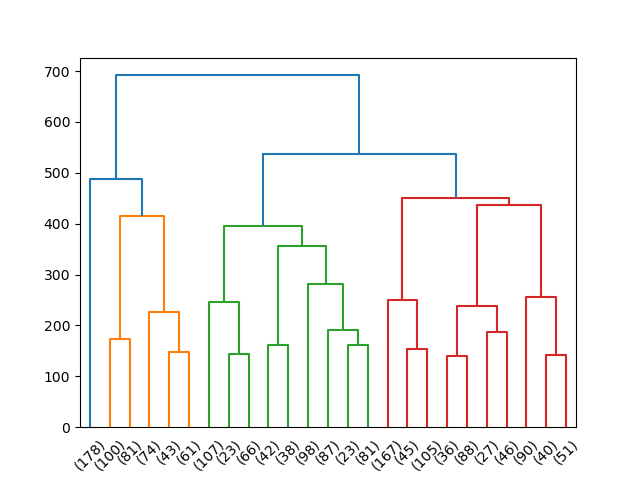
\includegraphics[width=0.24\linewidth]{graphics/dendrogram_ward.png}
    \caption{Dendrograms of agglomerative hierarchical clustering trees trained on the \texttt{digits} dataset from sklearn, using the complete,single,average and Ward linkage.}
    \label{fig:dendro}
\end{figure}



\subsection{Recommended further reading and exercises}
Unsupervised learning is treated in Chapter 12 of Introduction to statistical learning - clustering is more specifically treated in section 12.4. Recommended exercises are 12.6.2 and 12.6.4. Also consider the following exercise:

\begin{exercise}
    Prove that the Ward linkage can be defined through \eqref{eq:ward_linkagew}.
\end{exercise}







   

\section{Learnability theory}
Let us end the lecture where we started -- at the heart of the theory of statistical learning. Remember the setting: we are trying to determine a function $f_*$ from (noisy) samples $(f_*(x_i))_{i \in [m]}$, where $x_i$ are drawn from a set according to some probability distribution. We want to determine an estimate $f$ of $f_*$ from the samples $f_*(x_i)$. We have during the course learnt many ways to do so, but we have yet to pose the fundamental question of \emph{when this even is possible}. And if it is possible, how \emph{hard is it}? 

A framework in which such questions can be asked is the framework of \emph{Probably Approximately Correct} learning, or PAC-learning.
We will present it here in the context of binary classification, which is the cleanest and most classical one. To explain what PAC learning is, let us first present some terminology.
\begin{defi}
    Let $X$ be a set. 
    \begin{itemize}
        \item A \emph{target function} or \emph{target concept} is a function $f:X \to \{0,1\}$. A set of target concepts $C$ is a \emph{concept class}. 

        \item A \emph{sample of $f_*$} of size $m$ is a set $(x_i)_{i \in [m]}\sse X$ together with its values $(f_*(x_i))_{i \in [m]}$. The set of all samples of any size from any function in the concept class $C$ is denote $\calS_C$.

        \item Let $H$ be a set of potential concepts, a \emph{hypothesis class}. A map $\calA : \calS_C \to H$ is an \emph{algorithm}.

        \item An algorithm is \emph{consistent for the class $C$} if its hypothesis always agree on the training examples. That is, if $h= \calA((x_i,y_i)_{i \in [m]})$ for some $(x_i,y_i)_{i \in [m]} \in \calS_C$,  $h(x_i)=y_i$ for all $i$.

        \item For a probability distribution $\mathbb{P}$ on $X$, the \emph{error of learning algorithm $\calA$ for a concept $f_*$ on a sample $\overline{x} = (x_i,f_*(x_i))_{i \in [m]}$ with respect to $\mathbb{P}$} is
        \begin{align*}
            e_{\calA,f_*,\mathbb{P}}(\overline{x}) = \mathbb{P}(f_*(x)\neq \calA(\overline{x})(x)).
        \end{align*}
        In short, the error is the test-error of the model $h$ trained on the sample $\overline{x}$ using $\calA$ and the test examples are distributed according to $\mathbb{P}$. If the concept and probability distribution is clear, we will also speak of the \emph{error of $h$}. 
    \end{itemize}
\end{defi}
\paragraph{Example: Linear classifiers}    Let us discuss these concepts in the case of training linear classifier.

    The set $X$ is here $\R^n$. The hypothesis class $H$ is the set of all functions of the form
    \begin{align*}
        h_{\alpha}(x) = \begin{cases}
            1 \text{ if } \sprod{\alpha,x} \geq 1  \\
            0 \text{ else}.
        \end{cases},
    \end{align*}
    where $\alpha\in \R^p$.

    We know a prominent model for learning linear classifiers: support vector machines. Training an SVM is an algorithm in the sense we have given above -- given any samples, we can apply it, get a hyperplane, and from that construct a decision function. Is the algorithm consistent? The classical (Hard-margin) SVM is! To train a hardmargin SVM, we optimize the margin among all hyperplanes that separate the classes. 'The hyperplane separates the classes' exactly means that all training examples are correctly classified by the decision function. Hence, the classical SVM is consistent.

    However, if we apply the soft margin SVM, it may very well be that be best hyperplane is not actually separating the data. Hence, the soft margin SVM is \emph{not} consistent.

   
\
    



Now let us come back to the concept of learnability. A class being PAC learnable means that there exists a learning algorithm that, when given enough samples, drawn according to a probability distribution $\mathbb{P}$, will with high probability output an hypothesis $h$ with a small error, when measured according to the same distribution. Let us define these concepts formally.
\begin{defi}
    \begin{itemize}
        \item Let $m$ be a function of $\epsilon$ and $\delta$ and let $\mathbb{P}$ a probability distribution on $X$. We say that $\calA$ is a \emph{learning algorithm for $C$ with respect to $\mathbb{P}$ with sample size $m(\epsilon,\delta)$} if  $\forall \, \epsilon>0 , \delta>0 \forall \, f_* \in C$
        \begin{align*}
          \mathbb{P}( e_{\calA,f_*,\mathbb{P}}(\overline{x}) >\epsilon)<\delta,
        \end{align*}
        where $\overline{x}$ is formed by drawing $m(\delta,\epsilon)$ samples from $X$ according to $\mathbb{P}$. 

        If $\calA$ is a learning algorithm for $C$ with respect to any $\mathbb{P}$ with sample size $m(\epsilon,\delta)$, we call it a \emph{learning algorithm for $C$ with sample size $m(\epsilon,\delta)$.}
        \item $C$ is \emph{PAC-learnable} with sample size $m(\epsilon,\delta)$ if there exists a $H$ and a learning algorithm $\calA : \calS_C\to H$ with sample size $m(\epsilon,\delta)$. 
    \end{itemize}
\end{defi}

That was a lot. We will in the following get to know the definition better by considering three concrete examples.

\subsection{Example 1: SVM for a three-point set}
Let us begin by considering applying SVM for learning a fixed linear classifier $f_*$ as shown in Figure \ref{fig:gt_svm}. Let us consider a deliberately non-practical but illustrative case of $\mathbb{P}$ being the uniform distribution on three points show in the same figure.

\begin{figure} 
    \centering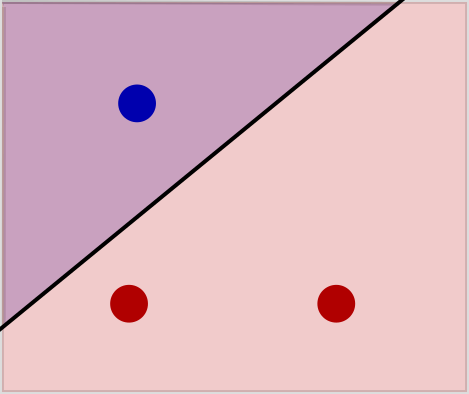
\includegraphics[width=0.5\linewidth]{graphics/ground_truth_svm.png}
    \caption{A ground truth linear classifier and a three point dataset.}
  \label{fig:gt_svm}
\end{figure}

\begin{figure} 
    \centering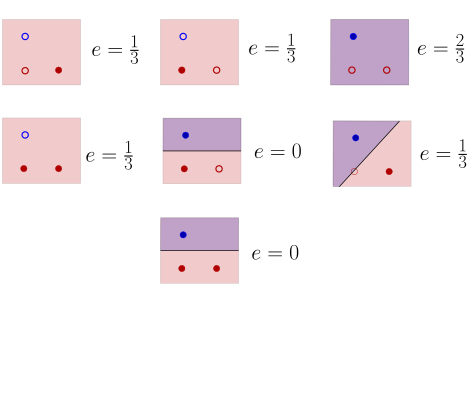
\includegraphics[width=0.5\linewidth]{graphics/error_svm.png}
    \caption{The error of the maximum-margin SVM depending on the sample. The points contained in the sample are filled, those excluded are not filled.}

    \label{fig:errors_svm}
\end{figure}

Since repeated samples with the same labels will not affect the SVM, there are now only $7$ different draws of the sample $\overline{x}$ that  drawn. For each one of these, we can determine the maximum margin hyperplane by inspection. For each one of these, we can then easily determine the error $e_{\calA,f_*,\mathbb{P}}(\overline{x})$. See Figure \ref{fig:errors_svm}. Note that the algorithm in none of the cases gives back the ground truth, but it does still have a zero error incertain cases.

Now, what can we say about the probability $\mathbb{P}(e_{\mathcal{A},f_*,\mathbb{P}}(\overline{x}) > \varepsilon)$? It heavily depends on the number of points drawn in the sample. If we draw two points, the three cases cases on the top of Figure \ref{fig:errors_svm} have probability $1/9$, the middle row cases have probabilities $2/9$ equiprobable. Since only one case will give us an error smaller than $1/3$, we will for any $\epsilon<\frac{1}{3}$, we will have $ \mathbb{P}( e_{\calA,f_*,\mathbb{P}}(\overline{x}) >\epsilon)= \tfrac{2}{9}$. If we however draw many points, we will will overwhelmingly big probability be in the case in the bottom row of Figure \ref{fig:errors_svm}: we can argue that if we draw $m$ points, the probability that we are not in that case is smaller than $3\cdot (2/3)^m$ (the probability that a certain dot is not drawn $m$ times is $(2/3)^m$, and there are three points that can be excluded). Hence, for any $\delta>0$
\begin{align*}
    \mathbb{P}( e_{\calA,f_*,\mathbb{P}}(\overline{x}) >\epsilon)\leq 3\cdot (2/3)^m,
\end{align*}
which is smaller than $\delta$ if $m \geq m \geq \log(2/3)^{-1}*\log(\delta/3)= \log(3/2)^{-1}\log(3/\delta)$.


By going through all other possible hyperplanes, we can conclude the same inequality for any other $f_*$. Hence, the SVM algorithm is in an algorithm for the class of linear classifiers for this $\mathbb{P}$ with a sample size $\log(3/2)^{-1}\log(3/\delta)$.

\subsection{Example 2: Finite intervals} 
Consider the class of finite intervals:
\begin{align*}
    C_{\mathrm{int}} = \{ \one_{[a,b]} \, \vert \, a,b \in \R\}.
\end{align*}
This is an infinite set, but we claim that it is still PAC learnable. To do so, consider the following simple learning algorithm:
\begin{align}
    \calA(\overline{x}) =\one_[c,d], \  c=\min \{x_i \, \vert \, y_i>1\}, d= \max \{x_i \, \vert \, y_i>1\}. \label{eq:track-alg}
\end{align}
That is, in words, just keep track of the smallest and largest positive examples in the sample, and output that interval. Note that this learning algorithm is consistent, and its hypothesis class is $C_{\mathrm{int}}$. We claim that this is a learning algorithm for $C_{\mathrm{int}}$ with sample size $2/\epsilon \log(2/\delta)$.
\begin{theorem}
    \eqref{eq:track-alg} is a learning algorithm for $C_{\mathrm{int}}$ with sample size  $2/\epsilon \log(2/\delta)$.
\end{theorem}
\begin{proof}
    Let $f_*= \one_{[a,b]} \in C_{\mathrm{int}}$, and $\overline{x}$ a sample.  Let us write $\mathcal{A}(\overline{x})=f=\one_{[c,d]}$ and define two sets
    \begin{align*}
        L = [a,\alpha], &\quad \alpha = \inf \{\alpha \, \vert \,  \mathbb{P}([a,\alpha])\geq \frac{\epsilon}{2}\} \\
        R = [\beta, b], &\quad \beta = \sup \{ \beta \, \vert \, \mathbb{P}([\beta,b])\geq \frac{\epsilon}{2}\},
    \end{align*}
    i.e. the smallest 'cut-outs' on the left and right of $[a,b]$ so that the probability of an $x$ lying there is bigger than $\frac{\epsilon}{2}$. Note that if no such cut-outs exist , $\mathbb{P}([a,b])\leq \epsilon$, and $\calA(\overline{x})$ will always have an error smaller than $e$ (since the only possible misclassification that can occur is that $x \in [a,b]$ but $\calA(\overline{x})(x)=0$). 

    Now, if the sample $\overline{x}$ contains at least one point $x_i$ in $\overline{x}$ in $L$ and one in $R$, the error of $\calA(\overline{x})$ is smaller than $\epsilon$ -- again,  $x$ is only misclassified by $f$ when when $x\in [a,c[ \cup ]d,b]$, and that set has a probability smaller than $\epsilon$ if $d\geq \beta$ and $\alpha\leq c$. Hence, the error of $f$ is bigger than $\epsilon$ only if all $x_i$ lie outside $L$ and outside $R$. Now, the probability of an $x_i$ lying outside $L$ is not bigger than $(1-\epsilon/2)$. Hence, the probability that all independently drawn $m$ lie outside the set is not bigger than $(1-\epsilon/2)^m$. The same bound holds for no samples lying in $R$. Hence, 
    \begin{align*}
        \mathbb{P}({e_{\calA,f^*,\mathbb{P}}}(\overline{x})>\epsilon) \leq \mathbb{P}(\forall \, i : x_i \notin L)  + \mathbb{P}(\forall \, i : x_i \notin R) \leq 2\left(1-\tfrac{\epsilon}{2}\right)^m\leq 2e^{-m\epsilon/2},
    \end{align*}
    where we used the inequality $e^{-x}\geq 1-x$. Hence, if $m\geq \tfrac{2}{\epsilon}\ln(\tfrac{2}{\delta})$, the probability of an error larger than $\epsilon$ is smaller than $\delta$. The claim has been proven.
\end{proof}
The above example can be generalized to  $n$ dimension -- the class of hypercubes $[a_0,b_0] \times \dots \times [a_{n-1},b_{n-1}]$ is also PAC-learnable with a sample size $\tfrac{2n}{\epsilon}\ln(\tfrac{2n}{\delta})$

\subsection{Example 3: Finite concept classes} 
Now let us consider a quite general example -- any concept class of finite size, $C= \{f_0, \dots, f_{K-1}\}$. Here, an obvious learning algorithm is to simply pick any of the $f_\ell\in C$ that are consistent with the sample $\overline{x}$, i.e. 
\begin{align*}
    \calA(\overline{x}) = \text{Uniformly random draw from } \{f \in C : f(x_i) = y_i, (x_i,y_i)\in\overline{x}\}.
\end{align*}
(One such $f_i$ must exists, since the sample is done without error). This is in fact a learning algorithm with (for fixed $\epsilon$ and $\delta$) sample size proportional to $\ln(\abs{C})$! This follows from the following
   \begin{theorem}
        Let $C$ be finite. If an algorithm $\calA: \calS_C \to C$ is consistent, it is a learning algorithm for $C$ with sample size 
        \begin{align*}
             \tfrac{1}{\epsilon} \ln \left(\frac{\abs{C}}{\delta}\right).
        \end{align*}
    \end{theorem}
    \begin{proof}
        Let $f_*\in C$ and $\mathbb{P}$ be arbitrary, and let $h\in C$ be a hypothesis with error bigger than $\epsilon$, i.e.
        \begin{align*}
            \mathbb{P}(f(x)\neq h(x))>\epsilon.
        \end{align*}
        $h$ will be inconsistent with $f_*$ on a sample $\overline{x}$ unless all $x_i$ are such that $f(x_i)=h(x_i)$. The probability that $f(x_i)=h(x_i)$ is less than $1-\epsilon$, so the the probability that all $f(x_i)=h(x_i)$ is less than $(1-\epsilon)^m\leq e^{-m\epsilon}$. Hence, the probability that $h$ is consistent with $f$ is less than $e^{-m\epsilon}$.

        Now, there will (trivially) be less than $\abs{C}$ hypotheses in $C$ that have an error bigger than $\epsilon$. Hence, by a union bound,
        \begin{align*}
            \mathbb{P}(\exists \, h \text{ consistent with $f_*$ on $\overline{x}$ and with error greater than $\epsilon$ }) \leq \abs{C}e^{-m\epsilon}<\delta
        \end{align*}
        if $m \geq \tfrac{1}{\epsilon} \ln \left(\frac{\abs{C}}{\delta}\right)$. However, if there are no $h\in C$  consistent with $f_*$ on the and with error greater than $\epsilon$, the $h$ picked by $\calA$ must have an error smaller than $\epsilon$. Hence, $\mathbb{P}(e_{\calA,f_*,\mathbb{P}}>\epsilon)<\delta$, i.e., the claim. 
    \end{proof}
%\begin{theorem}[Hoeffding's inequality]
%    Let $z_i$ be $m$ independently and identically variables on $[0,1]$, with (common) expected value $\erw(z)$. Then
%    \begin{align*}
%        \mathbb{P}\big(\big\vert\tfrac{1}{m}\sum_{i \in [m]} z_i - \erw(z)\big\vert \geq t\big) \leq 2e^{-\tfrac{mt^2}{2}}
%    \end{align*}
%\end{theorem}
%\begin{proof}
%    First, let $T$ be real-valued random variable. It is clear that the indicator function $\one_{\R^+}(t)$ of the positive real line is pointwise smaller than $\exp(t)$. Therefore, for any $\alpha>0$
%    \begin{align*}
%        \mathbb{P}(T>0) =  \mathbb{P}(\alpha T>0) \erw(\one_{\R^+}(\alpha T)) \leq \erw\exp(\alpha T).
%    \end{align*}
%   Now write $\overline{z}_i = z_i - \erw(z)$. By the above, we have
%    \begin{align*}
%        \mathbb{P}\big(\tfrac{1}{m}\sum_{i \in [m]} \overline{z}_i \geq t\big) = \mathbb{P}\big(\sum_{i \in [m]} \overline{z}_i -mt\geq 0\big) \leq \mathbb{E}\big(\alpha\sum_{i \in [m]} \overline{z}_i -m \alpha t\big) = e^{-m\alpha t} \prod_{i \in [m]} \erw(\exp(\alpha\overline{z_i})),
 %   \end{align*}
  %  where we used that the $z_i$ are independent. Now, by assumption, $\abs{\alpha\overline{z_i}}\leq 2\alpha$. Therefore,
   % \begin{align*}
    %    \alpha \overline{z_i} = t(-2\alpha) + (1-t)2\alpha
    %\end{align*}
    %for $t = \frac{2-\overline{z_i}}{4} \in [0,1]$. Convexity of $\exp$ therefore gives
    %\begin{align*}
     %   \exp(\alpha\overline{z_i}) = \exp(t(-2\alpha)+(1-t)2\alpha)\leq te^{-2\alpha} + (1-t) e^{2\alpha} = \frac{2-\overline{z_i}}{4} e^{-2\alpha} + \frac{2+\overline{z_i}}{4} e^{2\alpha}
    %\end{align*}
    %Taking the expectation here, and $\erw(\overline{z}_i)=0$, yields
    %\begin{align*}
     %   \erw( \exp(\alpha\overline{z_i})) \leq \tfrac{1}{2}(e^{-2\alpha}+e^{2\alpha}) = \sum_{k=0}^\infty \frac{1}{2}\cdot \left(\frac{(2\alpha)^k}{k!}+\frac{(-2\alpha)^k}{k!}\right) = \sum_{k=0}^\infty \frac{(2\alpha)^{2k}}{(2k)!} \leq  \sum_{k=0}^\infty \frac{2^2k(\alpha^2)^{k}}{2^kk!}= e^{2\alpha^2}.
    %\end{align*}
   %Hence
   %\begin{align*}
    %    \mathbb{P}\big(\tfrac{1}{m}\sum_{i \in [m]} \overline{z}_i \geq t\big) \leq (e^{2\alpha^2})^m\cdot e^{-2m\alpha t}= e^{2m\alpha^2-2m\alpha t}
   %\end{align*}
   %for any $\alpha$. By choosing $\alpha =t/2 $, we get a one-sided estimate -- the probability that can be bounded in the exacts same way, so that a union bound gives the claim.
   % \end{proof}

 %   Now let $z_i = \one_{f_\ell(x_i)\neq f_*(x_i)}$, where $f_\ell$ is an arbitrary but fixed member of $C$, and the $x_i$ are randomly sampled from a probability distribution $\mathbb{P}$. $z_i$ are clearly i.i.d variables on $[0,1]$. Furthermore, the expected value of $z_i$ is equal to 
 %   \begin{align*}
  %      e_\ell = \mathbb{P}\left( f_*(x) \neq f_\ell(x)\right).
   % \end{align*}
    %Hoeffding therefore implies
    %\begin{align*}
    %    \mathbb{P}\left( \abs{\tfrac{1}{n} \sum_{i \in [m]} \one_{f_\ell(x_i)\neq f_*(x_i)}-e_\ell}>t\right) \leq 2 e^{-\tfrac{mt^2}{2}}.
   % \end{align*}
    %Now, for the  $f_\ell$ that are eligible for being chosen by $\calA(\overline{x})$, $\one_{f_\ell(x_i)\neq f_*(x_i)}=0$ for all $i$. Hence, for those $\ell$, 
   % \begin{align*}
    %    \mathbb{P}\left( \abs{e_\ell}>\epsilon\right) \leq 2 e^{-\tfrac{m\epsilon^2}{2}}.
    %\end{align*}
    %In order for the error of $\calA(\overline{x})$, the above must be true for all $f_\ell$ consistent with the sample $\overline{x}$. There are however no more than $\abs{C}$ such $f_\ell$, so that a union bound yields
    %\begin{align*}
    %    \mathbb{P}\left( e_{\calA,f^*,\mathbb{P}} >\epsilon\right) \leq \mathbb{P} \left(\forall \, \ell : \abs{e_\ell}>\delta\right) \leq 2\abs{C} e^{-\tfrac{m\epsilon ^2}{2}},
    %\end{align*}
   % which is smaller than $\delta$ if $m\geq \tfrac{2}{\epsilon^2}\ln(\frac{2\abs{C}}{{\delta}})$. We conclude
 
    %\paragraph{Remark:} Using more complicated arguments, we can remove the square from the $\epsilon$.

\subsection{VC dimension}
We have seen that any finite concept class $C$ can be learned with a sample size (for fixed $\epsilon$ and $\delta$) proportional to $\ln(\abs{C})$. We also know that there are classes that are infinite that are PAC learnable. There is in fact a general concept which can be used to determine if a class is PAC learnable, and if so, with what sample size: the so-called \emph{VC dimension} of the class (VC stands for Vapnik-Chervonenki, the inventors of the concept).

\begin{defi}
    Let $C$ be a concept class and $S\sse X$ a subset. Let $C_S$ be the set of restrictions of $f\in C$ to $S$, i.e.
    \begin{align*}
        C_S = \{f:S \to {0,1} \, \vert \ f\in C\}.
    \end{align*}
    We say that $C$ \emph{shatters} $S$ if $C_S$ contains any function $S\to \{0,1\}$

    The cardinality of the largest finite set that is shattered by $C$ is called the \emph{VC-dimension} of $C$. If $C$ shatters arbitrarily large finite sets, the $VC$-dimension is infinite.
\end{defi}

\paragraph{Example} Consider the class of finite intervals $C_{\mathrm{int}}$. Any set of two points is shattered by $C_{\mathrm{int}}$, as the Figure \ref{fig:vcinterval} shows. However, a set of three points $a<b<c$ is not shattered -- no $f\in C_{\mathrm{int}}$ can achive $f(a)=1, f(c)=1$ but $f(b)=0$. Hence, the VC-dimension of ${\mathrm{int}}$ is equal to $2$.

\begin{figure}
    \centering
    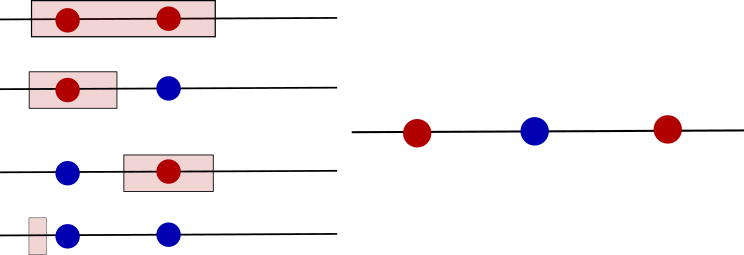
\includegraphics[width=0.6\linewidth]{graphics/VC_INTERVAL.png}
    \caption{The set of finite interval can generate all binary functions on two points, i.e., shatter it. It can however not generate the function visualized on the right.}
    \label{fig:vcinterval}
\end{figure}

\paragraph{Example} Trivally, if $C$ is finite, the number of functions in $C_S$ is smaller than $\abs{C}$. Since the total number of binary functions $S\to {0,1}$ is equal to $2^{\abs{S}}$, we see that $C$ cannot shatter $S$ if $\abs{C}\leq 2^{\abs{S}}$, i.e. $\abs{S}\geq \log_2(\abs{C})$. An upper bound of the VC dimension is hence $\log_2(\abs{C})$

\paragraph{Example} Let us consider a slightly more complicated example: The class of hyperplanes in $\R^{d}$ 
\begin{align*}
    C_{\mathrm{hyp}} = \{ f(x) = \one_{\sprod{\beta,x}+c>0} \, \vert \, \beta\in \R^d, c \in \R\}.
\end{align*}
We claim that the $VC$-dimension of this class is equal to $d+1$.

\underline{(a) The VC-dimension is at least $(d+1)$} Remember that the VC-dimension is defined as the cardinality of the largest set the class can shatter. Therefore, it suffices to construct a set of size $(d+1)$ that $C_{\mathrm{hyp}}$ can shatter. This is however easy -- take $x_0$ as the origin and $x_1, \dots x_d$ as the canonical basis vectors, and let $y_i \in \{0,1\}$ be arbitrary. Define
\begin{align*}
    w = [y_1-1/2, \dots, y_d-1/2], \quad  c = y_0/2.
\end{align*}
Then
\begin{align*}
    \one_{\sprod{w,x_0}+c>0} &  \one_{y_0/2>0} = y_0 \\
    \one_{\sprod{w,x_i}+c>0} &=  \one_{y_i -1/2 +  y_0/2>0} = \one_{2y_i + y_0>1} = \one_{y_i >0} = y_i,
\end{align*}
where we repeteadly used that $y_i$ are either $0$ or $1$. Hence, restricting the function corresponding to $w$ and $c$ to the set yields the function that maps $x_i$ to $y_1$.

\underline{(b) The VC-dimension is at most $(d+1)$} Now, we must argue that no set of size $d+2$ can be shattered. To do this, take any set $x_i \in \R^d$ with $d+2$ points and consider the points $\hat{x}_i = [1,x_i] \in \R^{d+1}$. Since there are $d+2$ points, there must be one $\hat{x}_i$ that can be expressed as a linear combinations of the others, WLOG $x_0$:
\begin{align*}
    x_i = \sum_{i\geq 1} a_i x_i.
\end{align*}
The $a_i$ cannot be all be zero, since $\hat{x}_0$ is not. Let us without loss of generality assume that there exists at least one $a_i$ with $a_i>0$ -- the case when all non-zero $a_i$ are negative is sensitive


Now, set $y_0= 0$, and for for $i \geq 1$, set the labels according to the signs of the $a_i$: If $a_i>0$, set $y_i=1$, and $y_i=0$ else. We claim that no function in $C_{\mathrm{hyp}}$ can realise the function $f(x_i)=y_i$. Suppose that there was. Then, 
\begin{align*}
  \sprod{\hat{w},x_i}
\end{align*}
must for all $i$ have the same sign as the $a_i$ -- if not, they would not be classified correctly (where we wrote $\hat{w}=[\beta,c]$ as usual). But then
\begin{align*}
   \sprod{\hat{w},x_0} = \sum_{i\geq 1} a_i \sprod{x_i,\hat{w}} >0,
\end{align*}
since the sum only consists of non-negative numbers, and at least one is positive. This is a contradiction to $\hat{w}$ producing the label $0$ for $x_0$!

\paragraph{Example} The set of continuous functions on an interval $I$ clearly has VC dimension equal to $\infty$ -- for any set of points $x_i$ and values $y_i$, a piecewise linear function $\lambda$ with $x_i$ as functions and $\lambda(x_i)=y_i$ realises the function $f(x_i)=y_i$, and is in the class of continuous functions.

\subsection{The 'fundamental theorem' of PAC learning}

Why have we introduced the VC dimension? Because it distinguishes the classes that are PAC learnable!
\begin{theorem}
    $C$ is uniformly learnable from finitely many samples if and only if the $VC$-dimension of $C$ is finite.
    
    If the VC-dimension is equal to $d<\infty$, we furthermore have that any algorithm $\calA$ which is consistent on samples of $C$ is a learning algorithm for $C$, with sample size
    \begin{align*}
        \max \left(\frac{4}{\epsilon}\log\left(\frac{2}{\delta}\right), \frac{8d}{\epsilon}\ln\left(\frac{13}{\epsilon}\right)\right)
    \end{align*}
\end{theorem}

We will not prove the positive statement of this theorem, i.e. that a class is learnable if its VC dimension is finite. We will however prove the to some extent more surprising part -- that we \emph{cannot} learn a class with infinitely VC dimension. This follows immediately from the following.

\begin{prop}
    Suppose that the VC dimension of the class $C$ is greater than $d$. Then, for any hypothesis class $H$ and any algorithm $\calA: \calS_C\to H$, there exists a $\mathbb{P}$ so that 
    \begin{align*}
        \mathbb{P}(e_{\calA,f_*,\mathbb{P}}(\overline{x})>\epsilon)\geq 1/4.
    \end{align*}
    for $\overline{x}$ formed by drawing less than
    \begin{align*}
        m_* = d \left(\frac{1}{2} - \frac{3}{2}\epsilon\right)
    \end{align*}
    samples.
\end{prop}
\begin{proof}
    Since the VC dimension is $d$, there exists a set $S$ of size $d$ that is shattered by $C$. Let $\mathbb{P}$ be defined via drawing points from this set with uniform probability. Since both the errors and the values $f_*(x_i)$ of the samples for this probability distribution is independent of the values of functions outside $S$, we can from now on think about all functions as $f:S\to \{0,1\}$. As such, since $C$ shatters $S$, $C$ is equal to the entire set $\mathrm{Fun}(S)$ of functions $S\to \{0,1\}$.

    Now let $\calA: \calS_C \to H$ be an algorithm. When drawing $m_*$ points from $S$, there are at least $d-m^*$ points in $S$ that are unseen. This means that for any sample $\overline{x}=(x_i,y_i)_{i \in [m^*}$, there are at least $2^{d-m^*}$ functions $f\in \mathrm{Fun}(S)$ that could have caused it. No matter what the output $g=\calA(\overline{x})$ of the algorithm on that sample,  $f(x)\neq g(x)$ for at least half of the functions on each unseen point. When a point is drawn randomly according to $\mathbb{P}$, the probability that we land in an unseen point is $\frac{d-m^*}{d}$. Thus, the error of the algorithm averaged over all possible functions obeys
    \begin{align*}
       \forall \overline{x} :  \frac{1}{\abs{\mathrm{Fun}(S)}} \sum_{f \in \mathrm{Fun}(S)} e_{\calA,f,\P}(\overline{x}) \geq \frac{d-m^*}{2d}
    \end{align*}
    for each sample. The same bound then of course applies when we take the expectation over the sample $\overline{x}$. Fubini tells us that we may exchange the expectations, so that 
    \begin{align*}
        \frac{1}{\abs{\mathrm{Fun}(S)}} \sum_{f \in \mathrm{Fun}(S)} \erw_{\overline{x}}(e_{\calA,f,\P}(\overline{x})) \geq \frac{d-m^*}{2d}.
    \end{align*}
    This in particular shows that there is at least one $f_*$ with
    \begin{align*}
        \erw_{\overline{x}}(e_{\calA,f_*,\P}(\overline{x})) \geq \frac{d-m^*}{2d} \geq \frac{1}{4}+ \frac{3}{4}\epsilon
    \end{align*}
    Now it is only left to turn this into a lower bound on $p:=\mathbb{P}(e_{\calA,f_*,\mathbb{P}}(\overline{x})>\epsilon)$. Since $e_{\calA,f^*,\mathbb{P}}$ is smaller than one, we definitely have
    \begin{align*}
        \erw_{\overline{x}}(e_{\calA,f_*,\P}(\overline{x})) \leq 1 \cdot \mathbb{P}(e_{\calA,f_*,\P}(\overline{x})>\epsilon) + \epsilon \cdot \mathbb{P}(e_{\calA,f_*,\P}(\overline{x})\leq \epsilon) = p(1-\epsilon)+ \epsilon.
    \end{align*}
    Hence
    \begin{align*}
        \mathbb{P}(e_{\calA,f_*,\P}(\overline{x})>\epsilon) = p \geq \frac{1}{1-\epsilon}\left(\frac{1}{4}- \frac{\epsilon}{4}\right) = \frac{1}{4}.
    \end{align*}
\end{proof}

\subsection{Recommended reading and exercises}
There is no learning theory included in the coursebook. We recommend the lecture notes written by Dirk-André Deckert \cite{dirk2017lecture}
\href{https://www.mathematik.uni-muenchen.de/~deckert/teaching/SS17/ATML/media/VC_dimension.pdf}{to be found here}, for further reading. 

\begin{exercise}
    Consider the set of circles in the plane centered in the origin as a concept class $C_{\mathrm{circ}}$ of functions on the set $X= \R^2 \neq \{0\}$, i.e., excluding the origin. What is its VC-dimension?
\end{exercise}

\begin{exercise}
    Consider the set of fully connected networks (with an arbitrary number of layers and neurons per layer) as a concept class $C_{\mathrm{NN}}$ of functions on a bounded and closed interval. What is its VC-dimension?
\end{exercise}

\section{Non-linear dimensionality reduction methods}
% Multidimensional scaling
\subsection{Multidimensional scaling}
In Chapter 2, we discussed PCA, the by far most popular dimensionality reduction algorithm. We gave two interpretations of it: given data $X\in \R^{n,p}$, the principial directions describe (i) the $r$-dimensional subspace that best fits the data (ii) the $r$ direction in which the data $X$ varies the most. Let us start this chapter by giving a third interpretation. 

For a data-matrix $X$, let us define the \emph{centered similarities} $s_{ij} =\sprod{x_i-\overline{x},x_j- \overline{x}}$ as the inner product between the centered datapoints. Given a dimension $r$, we can now ask the question: Which $y_i\in \R^r$ best fits these similarities? More exactly, we can ask what the solution of 
\begin{align}
    \min_{Y\in \R^{n,r}} \sum_{i,j} \left(s_{ij} - \sprod{y_i-\overline{y},y_j-\overline{y}}\right)^2. \label{eq:classical_scale}
\end{align}
is. The answer is that it is the score-vectors corresponding to the $r$ first principial components.
\begin{theorem}
    The problem \eqref{eq:classical_scale} is solved by the eigenvectors to the $r$ biggest eigenvalues of the matrix $\overline{X}\overline{X}^T$, where $\overline{X}$ is the centered version of the data-matrix. That is, the problem is solved by calculating the $r$-dimensional score-vector associated to a PCA of $X$.
\end{theorem}
\begin{proof}
    We have $s_{ij}= \overline{X}\overline{X}^T$. The problem we are trying to solve is hence
    \begin{align}
        \min_{Y\in \R^{n,r}} \norm{\overline{X}\overline{X}^*-\overline{Y}\overline{Y}^*}_F^2, \label{eq:rankr}
    \end{align}
    where $F$ is the Frobenius-norm, i.e. $\ell_2$-norm for matrices.

    It is not hard to convince oneself (for instance by considering eigen-/Cholesky decompositions) that a matrix $M\in \R^{n,n}$ can be written as $YY^T$ for a matrix $Y\in \R^{n,r}$ if and only if it is symmetric and it has rank less than $r$. What we are looking for is hence the solution of the problem
    \begin{align*}
        \min_{\substack{\mathrm{rank}(M)\leq r  \\M\in \R^{n,n} \\ M \text{ sym.}}} \norm{XX^*-M}_F^2.
    \end{align*}
    Now remember that $\overline{X}\overline{X}^T = \Psi\Sigma \Psi^*$, where $\Psi$ contains the principal components as rows and $\Sigma$ is diagonal. It is not hard to show that
    \begin{align*}
       \norm{\overline{X}\overline{X}^*-M}_F = \norm{\Psi(\Sigma-\Psi^*M\Psi)\Psi^*}_F = \norm{
       \Sigma-\Psi^*M\Psi}_F.
    \end{align*}
    Now, $\mathrm{rank}(M)= \mathrm{rank}(\Psi^*M\Psi)=\mathrm{rank}(N)$, so that the problem \eqref{eq:rankr} is equivalent to 
    \begin{align*}
        \min_{\mathrm{rank}(N)\leq r} \norm{\Sigma-N}_F^2.
    \end{align*}
    This problem is however not hard to solve, since $\Sigma$ is diagonal -- we see that $N$ also must be diagonal, and that it must contain exactly the $r$ first eigenvalues (a formal argument proceeds by induction similar to the proof of Theorem \ref{th:svd} in Chapter 2), say $N=\Sigma_0^r$. Hence,  $M=\Psi\Sigma_0^r\Psi^*$ solves \eqref{eq:rankr}, and by some simple algebra this matrix is equal to $Z^r(Z^r)^*$, where $Z$ is the matrix of the $r$ first PCA scores.
\end{proof}

\paragraph{Multi dimensional scaling} The above theorem is interesting in that it gives a 'metric' interpretation of the SVD: It shows that the SVD gives the best way of choosing 'low-dimensional representatives' $y_i\in \R^r$ to mimic the similarities $s_{ij}$. Is this what we want from dimension reduction? About this we can argue, but it is clearly not the most natural thing to go after.  What do we want from a dimension reduction map $\Phi: \R^p \to \R^r$ is that $\Phi(x)\approx \Phi(x')$ if and only if $x\approx x'$. A mathematical way to express this is to say that the distance between $\Phi(x)$ and $\Phi(x')$ should be approximately the same as the distance between $x$ and $x'$ :
\begin{align} \label{eq:metric}
    \norm{\Phi(x)-\Phi(x')}_2 \approx \norm{x-x'}_2.
\end{align}
 This gives a natural idea: Instead of mimicking the similarities with the representatives, let's mimic the distances, i.e. to solve the following problem:
\begin{align*}
    \min_{Y \in \R^{n,r}} \sum_{i,j} (\norm{x_i-x_j}_2-\norm{y_i-y_j}_2)^2.
\end{align*}
This method is (the standard version of) \emph{multi-dimensional scaling}, sometimes also referred to as the \emph{Kruskal-Shephard} scaling. In contrast to PCA, 
there is no closed form solution of this problem, and one often resorts to either specialized iterative algorithms, or simply gradient descent, to solve it in practice. This causes it to be more expensive than PCA, but can give better results.




\paragraph{Remark} The problem \eqref{eq:classical_scale} that PCA solves called \emph{classical scaling}.

\

In many settings, there is more than one way to measure the distance between data-points. When the data lives in Euclidean spaces, resorting to the Euclidean norm is natural, but maybe not the best option. In other applications, the data may not live in Euclidean space -- think of text data, for instance -- and necessarily needs to be compared by other means. This is not a problem for multi-dimensional scaling -- even if the distances $d_{ij}= \mathrm{dist}(x_i,x_j)$ is not given by a norm, we can apply it without thinking.

What about classical scaling? It is less trivial to see, but one can in fact apply it with only the knowledge of the distances $d_{ij}$, in the following sense.
\begin{lemma}
    Let $\phi:\R^{n,n}\to \R^{n,n}$ denote the 'double centering map':
    \begin{align*}
        \phi(M) = (\id-\tfrac{1}{n}\one \one^*) M(\id-\tfrac{1}{n}\mathds{1}\mathds{1}^*).
    \end{align*}
    Then, if $D_{ij}=\norm{x_i-x_j}^2$ and $S_{ij} = \sprod{x_i-\overline{x},x_j-\overline{x}}$ for some vectors $x_i\in \R^p$, we have
    \begin{align*}
        S = -\tfrac{1}{2}\phi(D)
    \end{align*}
\end{lemma}
\begin{proof}
   To simplify the notation, let us write $C=\id-\tfrac{1}{n}\one \one^*$. We have $\overline{x}= \tfrac{1}{n}X^*\one$. Therefore, we can rewrite the centered matrix $\overline{X}$ as 
   $$X-\tfrac{1}{n}  \one (X^*\one)^* = X-\tfrac{1}{n}  \one\one^* X = CX.$$
    Consequently
    \begin{align*}
        S = \overline{X}\overline{X}^* = CXX^*C,
    \end{align*}
    where we in particular used $C=C^*$. Consequently, since $C^2=C$ ($C$ is the orthogonal projection onto the orthogonal complement of $\one$, $S=CSC$.
    
    Now, let us notice that
    \begin{align*}
        D_{ij}= \norm{x_i-x_j}_2^2= \norm{\overline{x}_i-\overline{x}_j}_2^2 = \norm{\overline{x}_i}_2^2 + \norm{\overline{x}_j}_2^2 - 2\sprod{\overline{x}_i,\overline{x}_j} = (n\one^*+\one n^*-2S)_{ij},
    \end{align*}
    where we defined $n_i = \norm{\overline{x}_i}_2^2$. Consequently
    \begin{align*}
        CDC = C(n\one^*+\one n^*-2S)C = -2S,
    \end{align*}
    Since $C\one=0$ and therefore $\one^*C=0$. This is the claim.

    
   
\end{proof}
The benefit in applying classical scaling instead of 'standard'  multi-dimensional scaling is again that it is \emph{computationally} simpler -- the computational complexity is comparable to performing a PCA.


\subsection{Isomap} 
An important choice when applying a multi-dimensional scaling method is which distance to use on the data space $\R^p$. When the data is vector space valued, we already mentioned that the Euclidean distance is natural, but maybe not the best shot. To exemplify what we mean, let us consider the famous \emph{Swiss roll} (toy) data set (Fig. \ref{fig:swiss}). The points in this dataset apparently lie on a two-dimensional surface (manifold). By 'unrolling' the Swiss roll, we should be able to find a good, two-dimensional representation of it. However, because of the way the surface is embedded into $\R^3$, using a metric scaling method with Euclidean distance in the feature space will not cut it: Points close to the 'lower loops' will be measured as close, although they are very far away in the 'manifold distance'.

The \emph{Isomap} algorithm is an elegant way to mitigate this problem. The idea of the algorithm is simple: Given data, we begin by constructing a graph, connecting each point to its $k$ closest points (for some $k$, a hyperparameter of the method). To these closest points, the distance is defined as the same as in the Euclidean space. To any other points, however, we re-calculate the distance by computing shortest paths in the graph. In this manner, the distance is measured 'along the data' and hopefully will better capture the geometry of the dataset. See Figure \ref{fig:isodistance} . for an illustration. For speed, one often chooses the classical scaling method for the last step (this is the default in \texttt{sklearn}, for instance), but the algorithm can in principle also be applied with e.g. Kruskal scaling. 

The difference in applying Isomap and standard multidimensional scaling is striking for the Swiss roll -- again see Figure \ref{fig:swiss}.






\begin{figure}
    \centering
    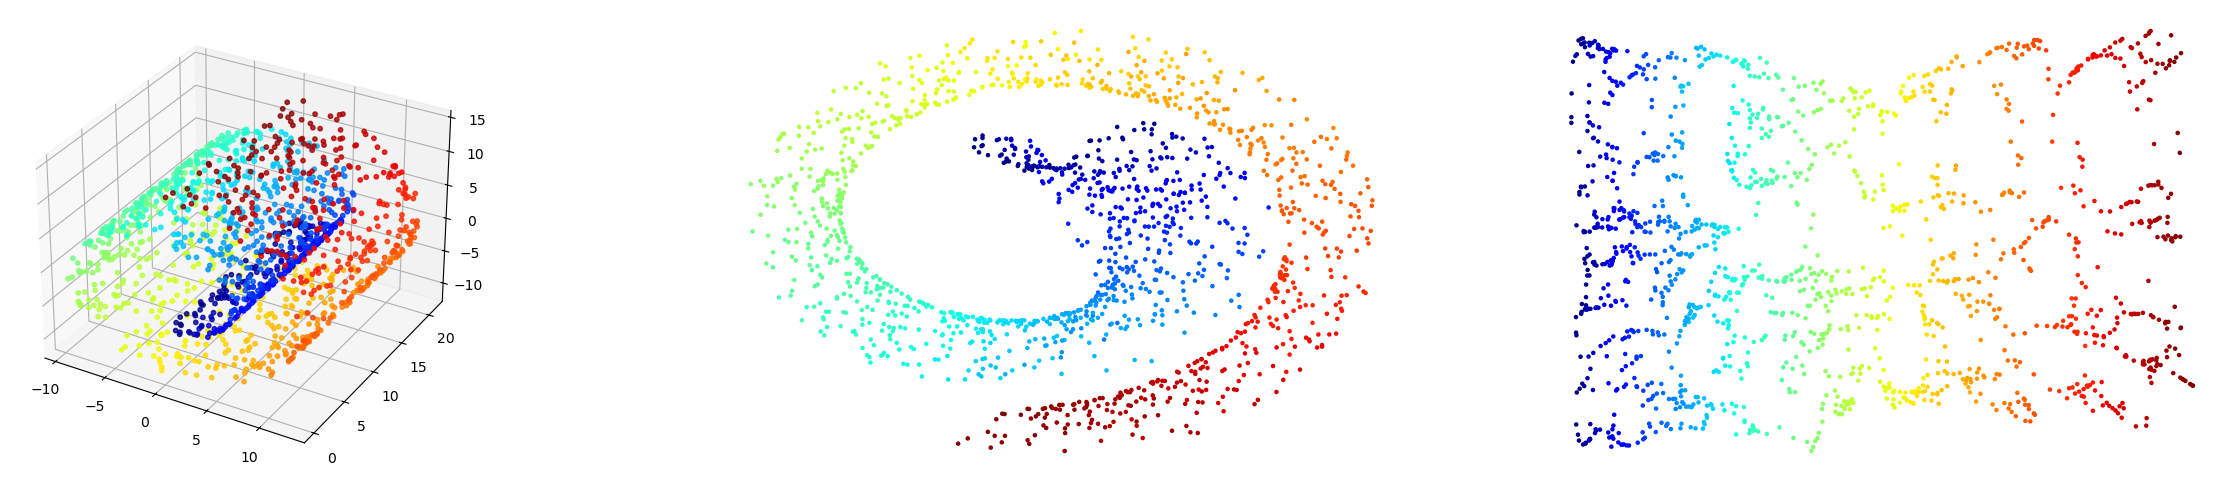
\includegraphics[width=0.85\linewidth]{graphics/swiss_roll.png}
    \caption{Left: the Swiss roll. Middle: The output of multi-dimensional scaling applied to the swiss roll. Right: The output of Isomap.}
    \label{fig:swiss}
\end{figure}

\begin{figure}
    \centering
    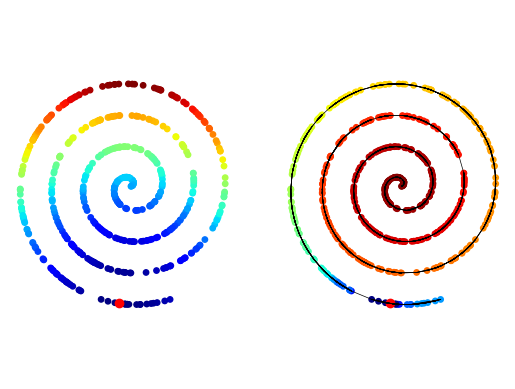
\includegraphics[width=0.5\linewidth]{graphics/distance_isomap.png}
    \caption{Left: A spiral, where the points have been color-coded according to the distance to the red point. Right. The same dataset, but with the $6$-nearest neighbor graph superimposed, and color codings according to the shortest path-distance in said graph.}
    \label{fig:isodistance}
\end{figure}


% ISOMAP

% Autoencoders

\subsection{Autoencoders}
Let us end this chapter by discussing a completely different approach to dimensionality reduction: the so-called \emph{autoencoder} idea. To get to this idea naturally, let us forget the 'metric' desideratum \eqref{eq:metric} for a moment, and instead follow another principle: A dimension-reduction method is \emph{only good if little information is lost}. That is, there should exist a way to \emph{decode} the dimension reduction map $\Phi$
\begin{align*}
    \exists \, \Delta: \R^r \to \R^p : \Delta \circ \Phi(x_i) = x_i \text{ for all data $x_i$.}
\end{align*}
Note that the 'for all data' is crucial here -- if we want it to be true for all $x\in \R^p$, and want $\Delta$ and $\Phi$ to be reasonable (e.g. continuous), we will not be able to reduce the dimension ($r\geq p$ in that case).

\paragraph{Remark} We have in fact already seen a concept that can be used this way: compressed sensing. The 'dimension-reduction method' here is to simply multiply the data with a Gaussian random matrix. This will work if the $x_i$ are inherently sparse. The decoder here $\Delta$ is the LASSO. In fact, this simple idea is sometimes used to reduce computational complexity -- it is then often called \emph{sketching}. The main pro of this approach is that it is extremely cheap.

\

How do we use this idea to reduce the dimension of a concrete  is to \emph{set up models} $\Phi$ and $\Delta$ for a given dataset? The idea is simple: We simply set up statistical models $\Phi$ and $\Delta$, that we then train to satisfy $\Delta \circ \Phi(x_i)=x_i$ for the data by using a loss function
\begin{align*}
    R(\theta_\Phi,\theta_\Delta) = \sum_{i \in [n]}\ell(\Delta_{\theta_\Delta}(\Phi_{\theta_\Phi}(x_i)),x_i)
\end{align*} A well-suited model to use for the en- and decoders are neural networks. In fact, we can set up the auto-encoder as a single neural network, and simply interpret the 'early' layers as the encoder and the 'late' layers as the decoder. 

\begin{figure}
    \centering
    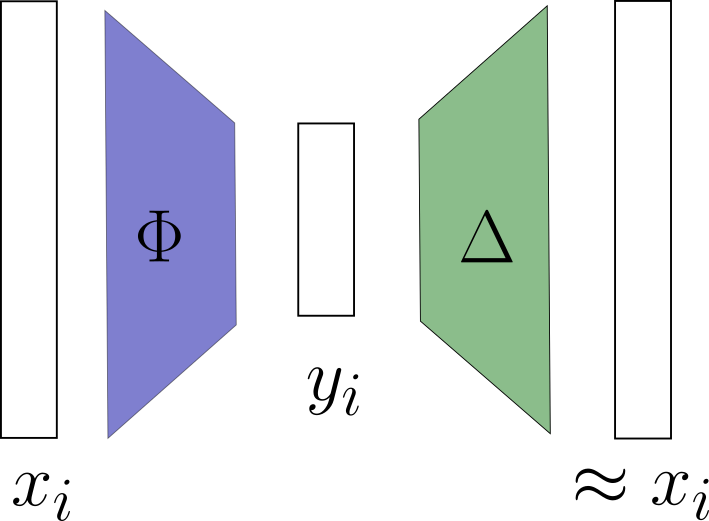
\includegraphics[width=0.5\linewidth]{graphics/auto_encoder_architecture.png}
    \caption{The idea of an autoencoder architecture}
    \label{fig:placeholder}
\end{figure}

\subsection{Autoencoders as generative models -- VAEs}
The encoder part of an autoencoder, as any other dimension reduction method, maps the data into a space into a \emph{latent space}. This latent space can be seen as an abstract vector space in which the data 'naturally lives'. What happens if now simply draw a point at random in this space, and use the decoder to reconstruct it? If the auto-encoder has spread out the data  into 'the whole' latent space $\R^r$, this point should be reasonably close to something in the data (or at least a point onto which a point in the underlying probability distribution would be mapped). Due to continuity of the decoder, it will therefore be decoded to something that is reasonably close to the data. Hence, we can use the decoder as a way to \emph{generate new data}!

If we train an autoencoder without any regularization, it is not very reasonable that the feature space is filled out. In more exact terms, it is not very reasonable that the representations $y_i=\Phi(x_i)$ are distributed according to some simple distribution $p$ (say, standard Gaussian), from which we easily can sample. The distribution we get from decoding $z_i$ we draw according to $p$ will then not resemble the distribution of the training data. If this is our main aim, we need to make sure this happen. A way to ensure this is to train a \emph{variational autoencoder}. 

The idea of the variational autoencoder is as follows: The encoder $\Phi$ maps each point $x$ to a point in the $\R^r$, but rather to a \emph{distribution} $q_{\Phi(x)}$ on $\R^r$. By running samples of $q_{\Phi(x)}$ through the decoder $\Delta$, we obtain a distribution of points on $\R^p$ again. We know train $\Phi$ and $\Delta$ to make sure that
\begin{itemize}
    \item $\Delta \circ \Phi(x) \approx \delta_x$ -- that is, the samples we get out of $\Delta \circ \Phi(x)$ are all very close to $x$. This we ensure by a term $\int\ell(x,\Delta(z))\mathrm{d} q_{\Phi(x)}(z)$ in the loss function. This can in general not be calculated exactly, of course, but we can easily 
    \item The distributions $q_{\Phi(x)}$ are all close to a prior distribution $p$ that we specify. We can for instance include a term $\mathrm{KL}(q_{\Phi(x)},p)$ in the loss -- the Kullback Leibler divergence from $q_{\Phi(x)}$ to $p$
\end{itemize}
In this way, drawing a point from $x$ and then sampling from $q_{\Phi(x)}$ will yield points in the feature space approximately distributed as $p$, and decoding samples from $p$ with $\Delta$ will generate a distribution of points on $\R^p$ close to the original data distribution.

Now, a neural network on a real computer of course cannot handle data distributions as infinite dimensional objects. We solve this by parametrizing them: A popular choice is to let the $q_{\Phi(x)}$ to be Gaussian, with a mean and variance $\mu(x),\sigma(x)$ that depend on $x$. The $\Phi(x)$-function in practice learns the functions $\mu(x)$ and $\sigma(x)$. This is also practical (1) since the KL-divergence between a general Gaussian and a prescribed standard Gaussian $p$ is simple to compute (2) the prescribed standard Gaussian distribution is simple to sample from.

\begin{figure}
    \centering
    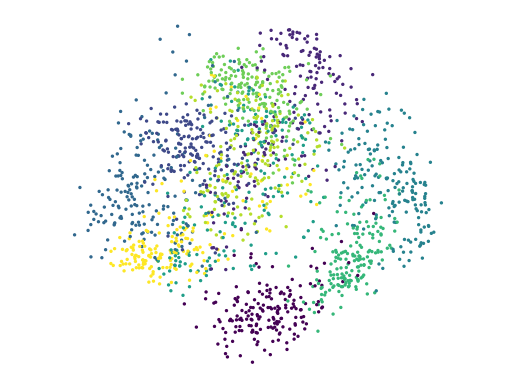
\includegraphics[width=0.2\linewidth]{graphics/pca.png}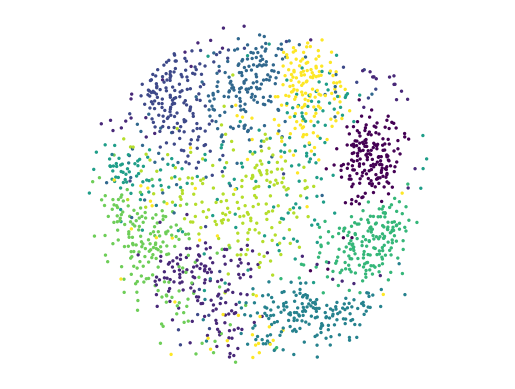
\includegraphics[width=0.2\linewidth]{graphics/mds.png}\includegraphics[width=0.2\linewidth]{graphics/isomap.png}\includegraphics[width=0.2\linewidth]{graphics/auto_encoder.png}\includegraphics[width=.2\linewidth]{graphics/variational_autoencoder.png}
    \caption{The result of applying (from left to right) PCA, MDS, Isomap, a (neural network) autoencoder and a (neural network) variational autoencoder to the \texttt{digits} dataset in \texttt{sklearn} to produce a two-dimensional representation of the data . (For the variational auto-encoders, we plot the means $\mu(x)\in \R^2$ to represent the distributions the encoder outputs). The colors correspond to the labels - these were however not used during training. We see that all methods put images of the same numbers close to each other, but they do it in slightly different ways.}
    \label{fig:placeholder}
\end{figure}

% variational autoencoders: https://arxiv.org/pdf/1906.02691
\subsection{Recommended further reading and exercises}
Non-linear clustering methods are not treated in the course book. Its more mathematical sibling, \emph{The elements of statistical learning} \cite{hastie2009elements} does so (in Chapter 14). The paper introducing the Isomap algorithm, \cite{tenenbaum2000global}, is a nice and short read, with a higher focus on application. A more thorough introduction to variational autoencoders, which however is quite mathematically heavy, can be found in \cite{kingma2019introduction}. 

\begin{exercise}
    Can PCA be turned into an autoencoder? Can multidimensional scaling be? Explain.
\end{exercise}

\begin{exercise}
    The hyperparameter $k$, the number of nearest neighbors in the graph, of Isomap is a tuneable parameter. Argue that if it is set very high, the output of Isomap will be essentially the same as PCA.
\end{exercise}

\bibliographystyle{IEEEtran}
\bibliography{stat_biography}
\end{document}